\section{Introduction}
Here motivation and status, references to results.

Do not forget \todo{reference Wjj benchmark}

\section{Setup}

\subsection{Colour Structures}
The gluon and fermion amplitudes \eqref{eq:defAmpsTens}
can be decomposed 
in terms of color structures. 
We denote the fundamental generators of the
$SU(\NC)$-group by $(T^a)^{\;\bar{\jmath}}_{i}$, where the
adjoint index $a$ runs over $\NC^2-1$ values and the 
(anti-) fundamental indices $i$  ($\bar \jmath$)
run over $\NC$ values. The fundamental generators are normalized
as $ \Tr(T^a T^b) = \delta^{ab}$. One can then consider the color decomposition of
each process as
%
\begin{align}
  \begin{split}
    \label{eq:ColorDecG}
    A(1_g, 2_g, 3_g, 4_g, 5_g) \big\vert_{\textrm{leading color}} = &
    \sum_{\sigma\in S_5/Z_5} \Tr\left(
    T^{a_{\sigma(1)}} T^{a_{\sigma(2)}} 
    T^{a_{\sigma(3)}} T^{a_{\sigma(4)}} T^{a_{\sigma(5)}} \right)\\
    &\times \CA({\sigma(1)}_g, {\sigma(2)}_g, {\sigma(3)}_g, {\sigma(4)}_g, {\sigma(5)}_g)\,, 
  \end{split} \\
  \begin{split}
    \label{eq:ColorDec2Q}
    A(1_q, 2_{\bar{q}}, 3_g, 4_g, 5_g) \big\vert_{\textrm{leading color}} 
    = & \sum_{\sigma\in S_3} 
    \left( T^{a_{\sigma(3)}} T^{a_{\sigma(4)}} T^{a_{\sigma(5)}} \right)^{\;\bar{\imath}_2}_{i_1} \\
    & \times\CA(1_q,2_{\bar{q}},\sigma(3)_g,\sigma(4)_g,\sigma(5)_g)\,,
  \end{split}\\
  \begin{split}
    \label{eq:ColorDec4Q}
    A(1_q, 2_{\bar{q}}, 3_Q, 4_{\bar{Q}}, 5_g)
    \big\vert_{\textrm{leading color}} 
    = & 
  %
    \,(T^{a_5})^{\;\bar{\imath}_{2}}_{i_{3}} \delta^{\;\bar{\imath}_{4}}_{i_{1}}\;
  %
    \CA(1_{q}, 2_{\bar{q}}, 5_g, 3_{Q}, 4_{\bar{Q}}) \,\,+  \\
  %
    & \,(T^{a_5})^{\;\bar{\imath}_{4}}_{i_{1}} \delta^{\;\bar{\imath}_{2}}_{i_{3}}\;
  %
    \CA(1_{q},2_{\bar{q}},3_{Q},4_{\bar{Q}},5_g) \,,
  \end{split}
\end{align}
where $S_n$ denotes all permutations of $n$ indices and 
$S_n/Z_n$ all non-cyclic permutations of $n$ indices. 
We write the particle type explicitly as a subscript, and all
remaining properties of each particle (momentum, helicity, 
etc.) are implicit. 

The $\CA$ in \cref{eq:ColorDecG,eq:ColorDec2Q,eq:ColorDec4Q} are
called partial amplitudes. For each of the amplitudes considered, all
partial amplitudes can be related to the others by exchanging external
legs, so only one partial amplitude is independent. These are expanded in a perturbative
expansion,
\begin{equation}
    \label{eq:partials} 
    \CA
    = g^{3}_0 \left(
        \CA^{(0)}
      + \frac{\alpha_0}{4\pi}\NC \CA^{(1)}
      + \left(\frac{\alpha_0}{4\pi}\right)^2\NC^2  \CA^{(2)} 
      + \mathcal{O}(\alpha_0^3)
      \right),
\end{equation}
where $\alpha_0=g_0^2/(4\pi)$ is the bare QCD coupling and 
$\CA^{(k)}$ denotes a $k$-loop partial amplitude. Each 
$\CA^{(k)}$ can be further expanded as a series in powers of 
$N_f/N_c$,
\begin{align}
  \label{eq:nfdecomposition} 
  \begin{split}
  \CA^{(1)} &= \CA^{(1)[N_f^0]} + 
  \frac{\NF}{\NC}\CA^{(1)[N_f^1]}\,, \\
  \CA^{(2)} &= \CA^{(2)[N_f^0]} +
  \frac{\NF}{\NC}\CA^{(2)[N_f^1]} +
  \left(\frac{\NF}{\NC}\right)^2\CA^{(2)[N_f^2]}\,.
  \end{split} 
\end{align}
We compute the coefficients $\CA^{(k)[N_f^l]}$, with $0\leq l\leq
k\leq2$, where only planar diagrams contribute as we work in the
leading-color approximation. In figs.~\ref{fig_parents5g},
\ref{fig_parents2q3g} and \ref{fig_parents4q1g} we give representative
diagrams for each of these contributions.

%%%%%%%%%%%%% FIGURE %%%%%%%%%%%%%%%%%%
\begin{figure}[ht]
  \begin{center}
    \begin{tikzpicture}[scale=.9]
    % 5 point masters
    \node at (0,0){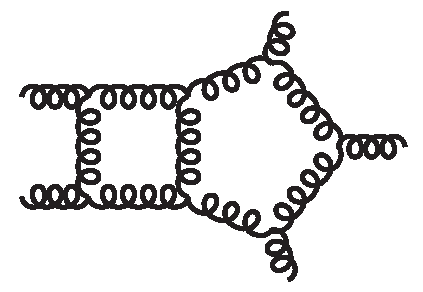
\includegraphics[scale=0.5]
    {figures/5g.pdf}};
    % 5 point masters
    \node at (5,0){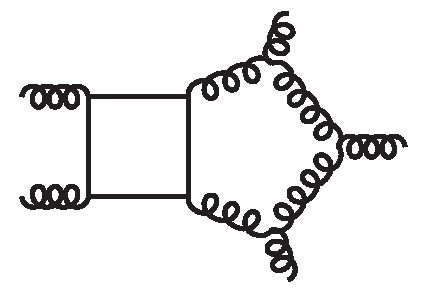
\includegraphics[scale=0.5]
    {figures/5gnf.pdf}};
    % Level 2 
    \node at (10,0){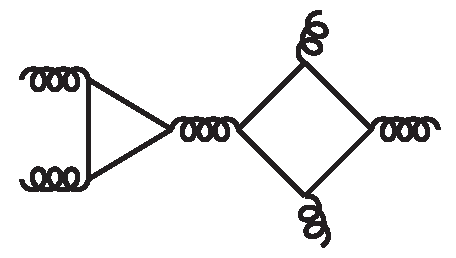
\includegraphics[scale=0.5]
    {figures/5gnf2.pdf}};
\end{tikzpicture}
\end{center} 
\caption{Representative Feynman diagrams for leading-color
$\CA^{(2)}(g,g,g,g,g)$ amplitudes, contributing at order
$N_f^0$, $N_f^1$ and $N_f^2$.}
\label{fig_parents5g}
\end{figure}

%%%%%%%%%%%%% FIGURE %%%%%%%%%%%%%%%%%%
\begin{figure}[ht]
  \begin{center}
    \begin{tikzpicture}[scale=.9]
    % 5 point masters
    \node at (0,0){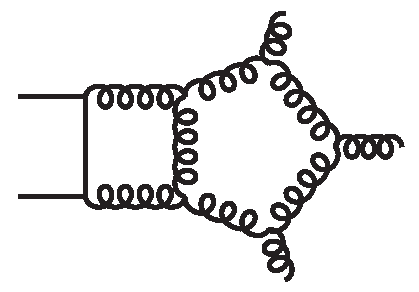
\includegraphics[scale=0.5]
    {figures/2q3g.pdf}};
    % 5 point masters
    \node at (5,0){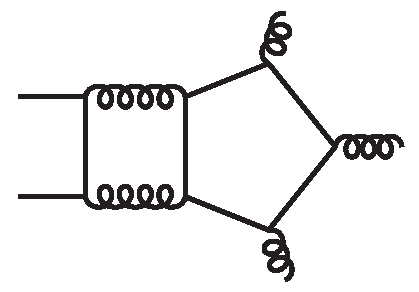
\includegraphics[scale=0.5]
    {figures/2q3gnf.pdf}};
    % Level 2 
    \node at (10,0){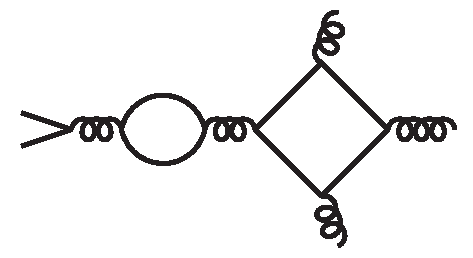
\includegraphics[scale=0.5]
    {figures/2q3gnf2.pdf}};
\end{tikzpicture}
\end{center} 
\caption{Representative Feynman diagrams for leading-color
$\CA^{(2)}(q,\bar q,g,g,g)$ amplitudes, 
contributing at order
 $N_f^0$, $N_f^1$ and $N_f^2$.}
\label{fig_parents2q3g}
\end{figure}

%%%%%%%%%%%%% FIGURE %%%%%%%%%%%%%%%%%%
\begin{figure}[ht]
  \begin{center}
    \begin{tikzpicture}[scale=.9]
    % 5 point masters
    \node at (0,0){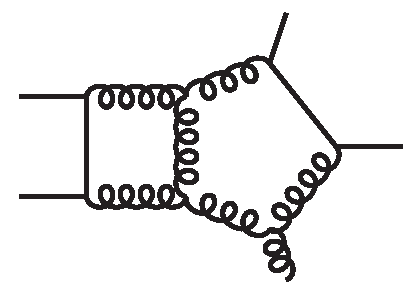
\includegraphics[scale=0.5]
    {figures/4q1g.pdf}};
    % 5 point masters
    \node at (5,.4){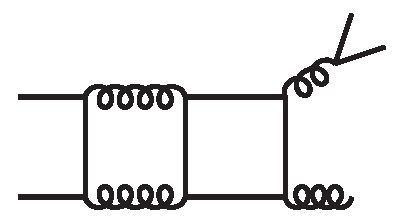
\includegraphics[scale=0.5]
    {figures/4q1gnf.pdf}};
    % Level 2 
    \node at (10,.4){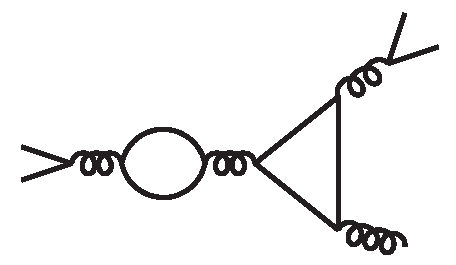
\includegraphics[scale=0.5]
    {figures/4q1gnf2.pdf}};
\end{tikzpicture}
\end{center} 
\caption{Representative Feynman diagrams for leading-color
$\CA^{(2)}(q,\bar q,Q,\bar Q,g)$ amplitudes, 
contributing at order
$N_f^0$, $N_f^1$ and $N_f^2$.}
\label{fig_parents4q1g}
\end{figure}


\subsection{Construction of Cut Equations}

\todo{here describe generation of hierarchies}

\subsubsection{Unitarity-Compatible Color Decomposition}
\todo{Process library belongs here or to the appendix?}
Here describe the approach of how process library does the colour decomposition.

%%%%%%%%%%%%% FIGURE %%%%%%%%%%%%%%%%%%
\begin{figure}[ht] 
  \begin{center}
    \begin{tikzpicture}[scale=1.1]
    % 5 point masters
      \node at (2.5,0){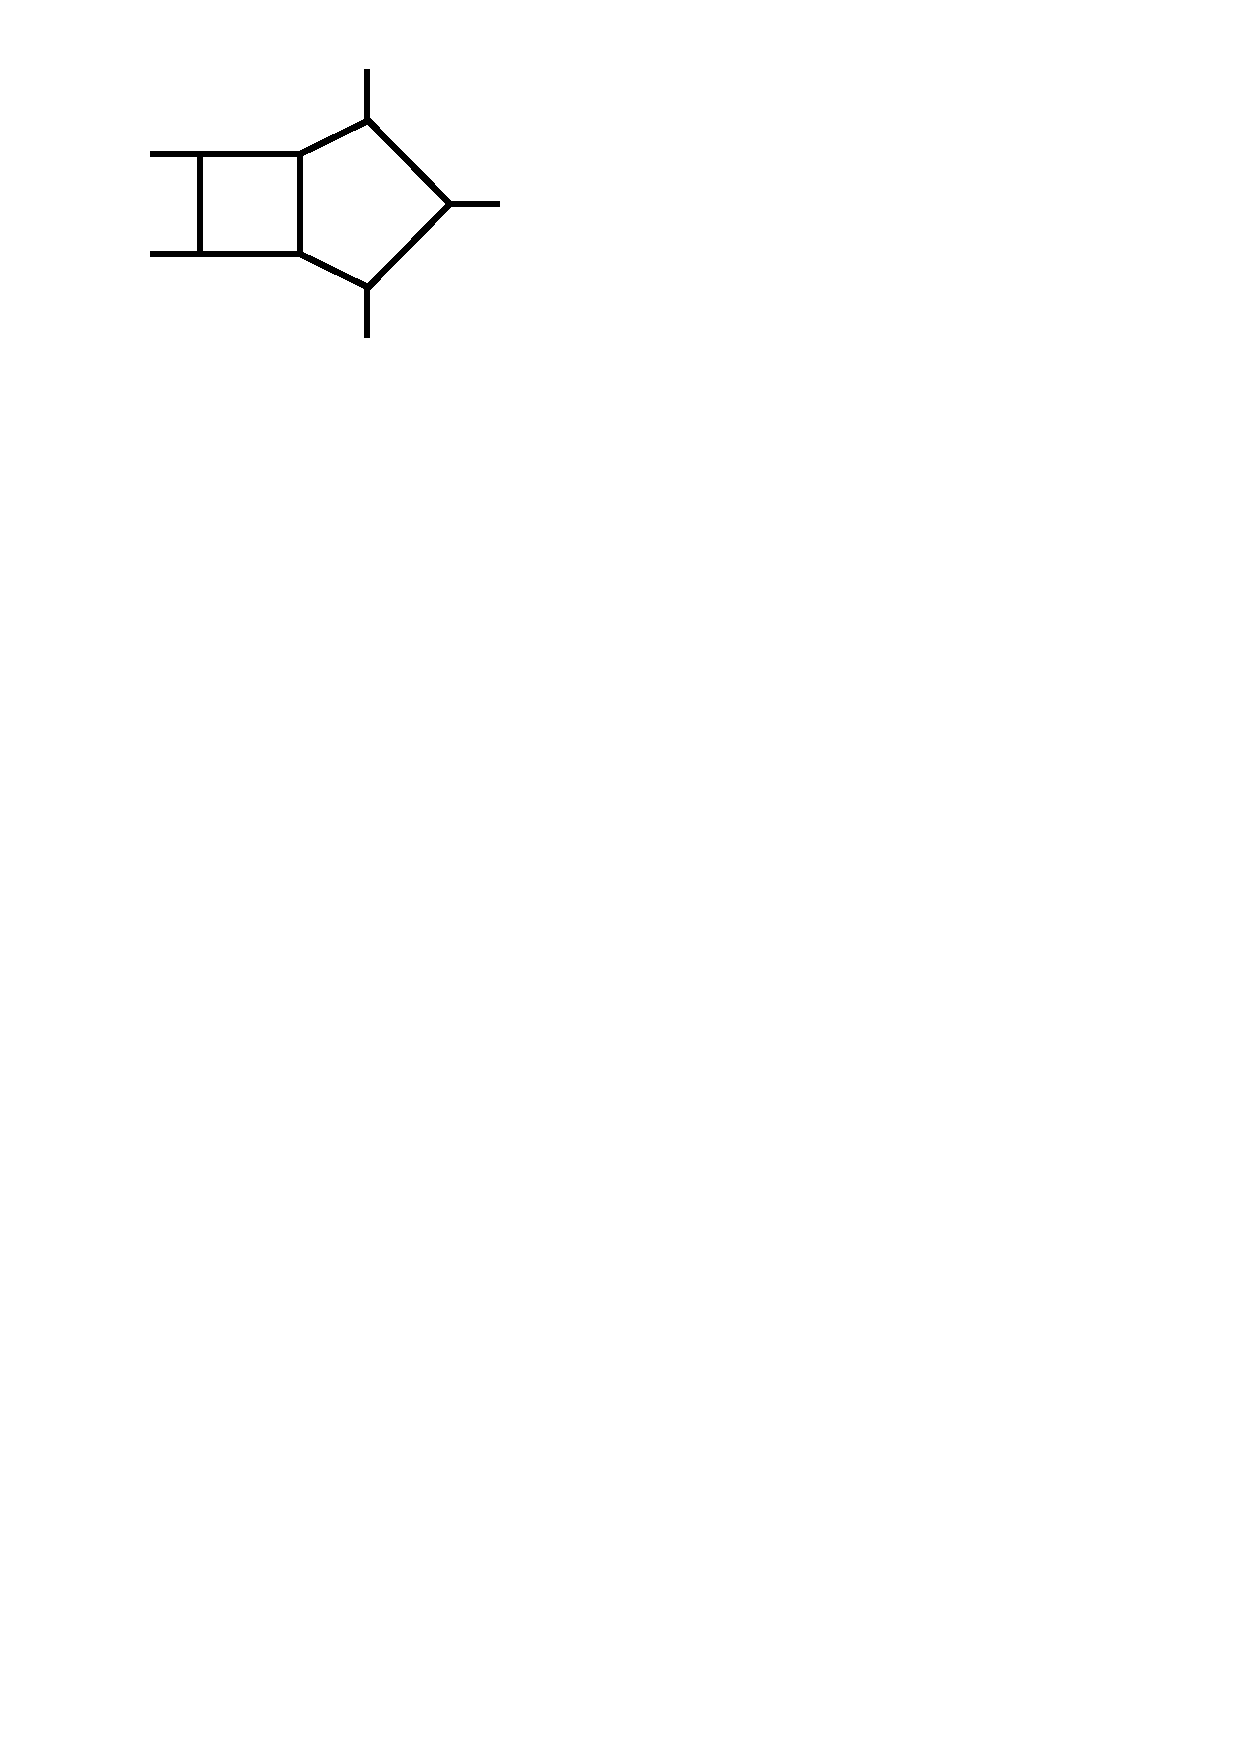
\includegraphics[scale=0.4]{figures/topologies/BoxPentagon}};
      \node at (5,0){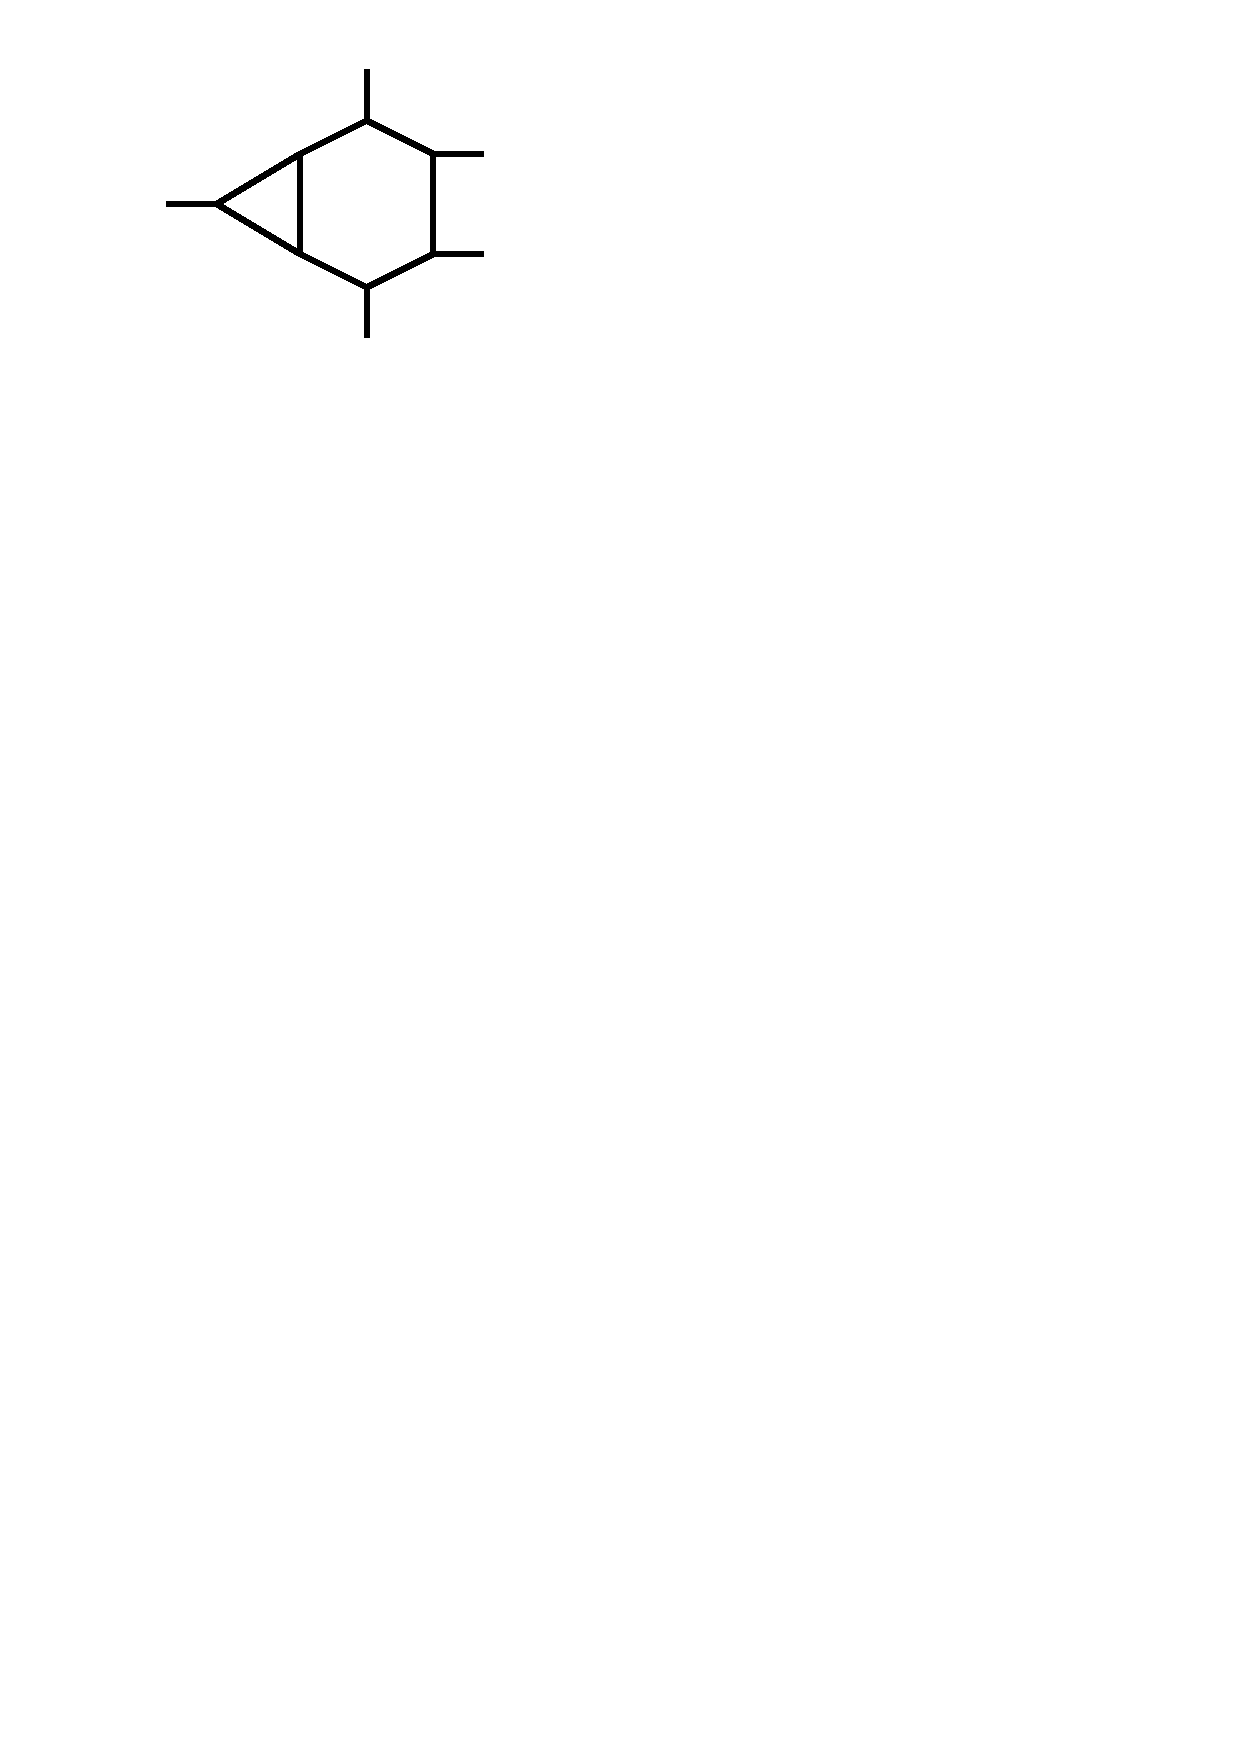
\includegraphics[scale=0.4]{figures/topologies/TriangleHexagonRed1}};
      \node at (7.5,0){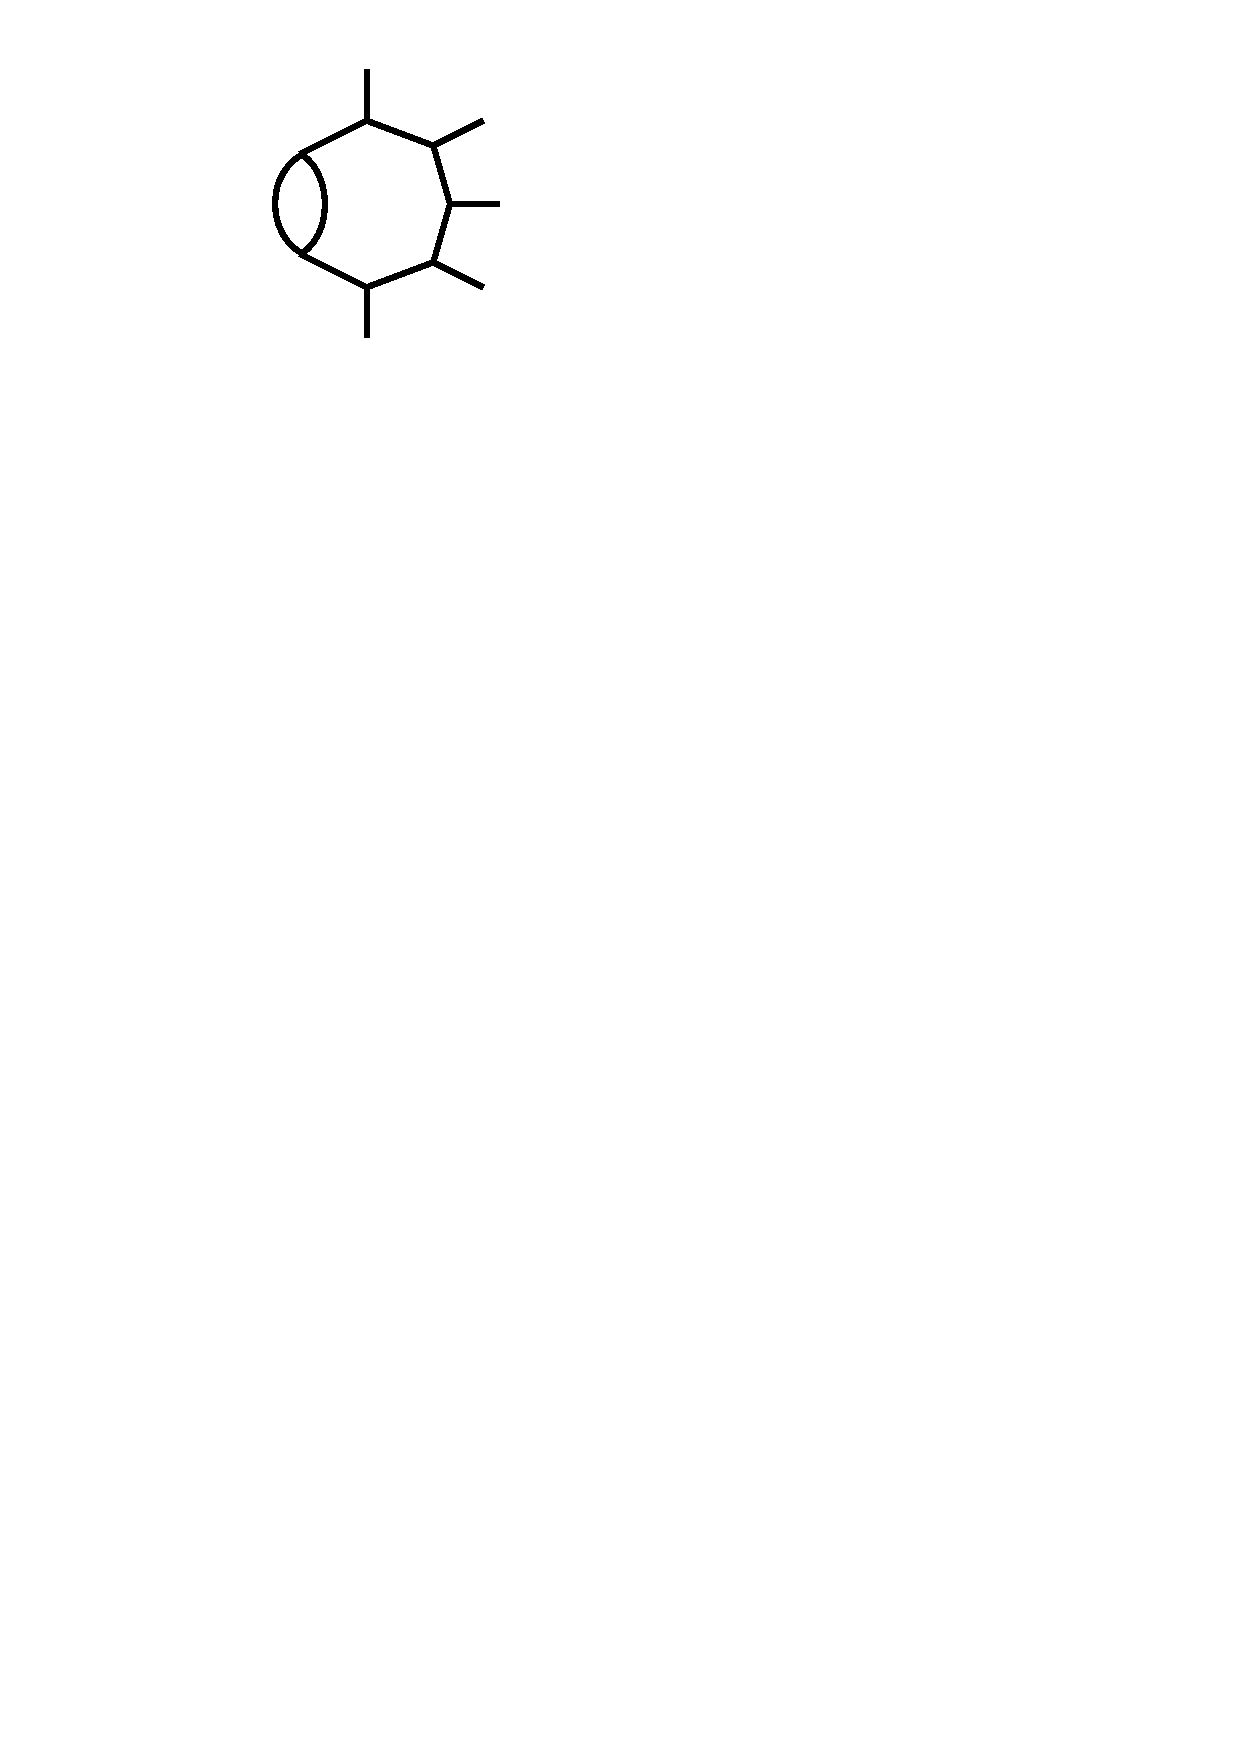
\includegraphics[scale=0.4]{figures/topologies/BubbleHeptagon}};
    % Level 2 
      \node at
      (0,-1.9){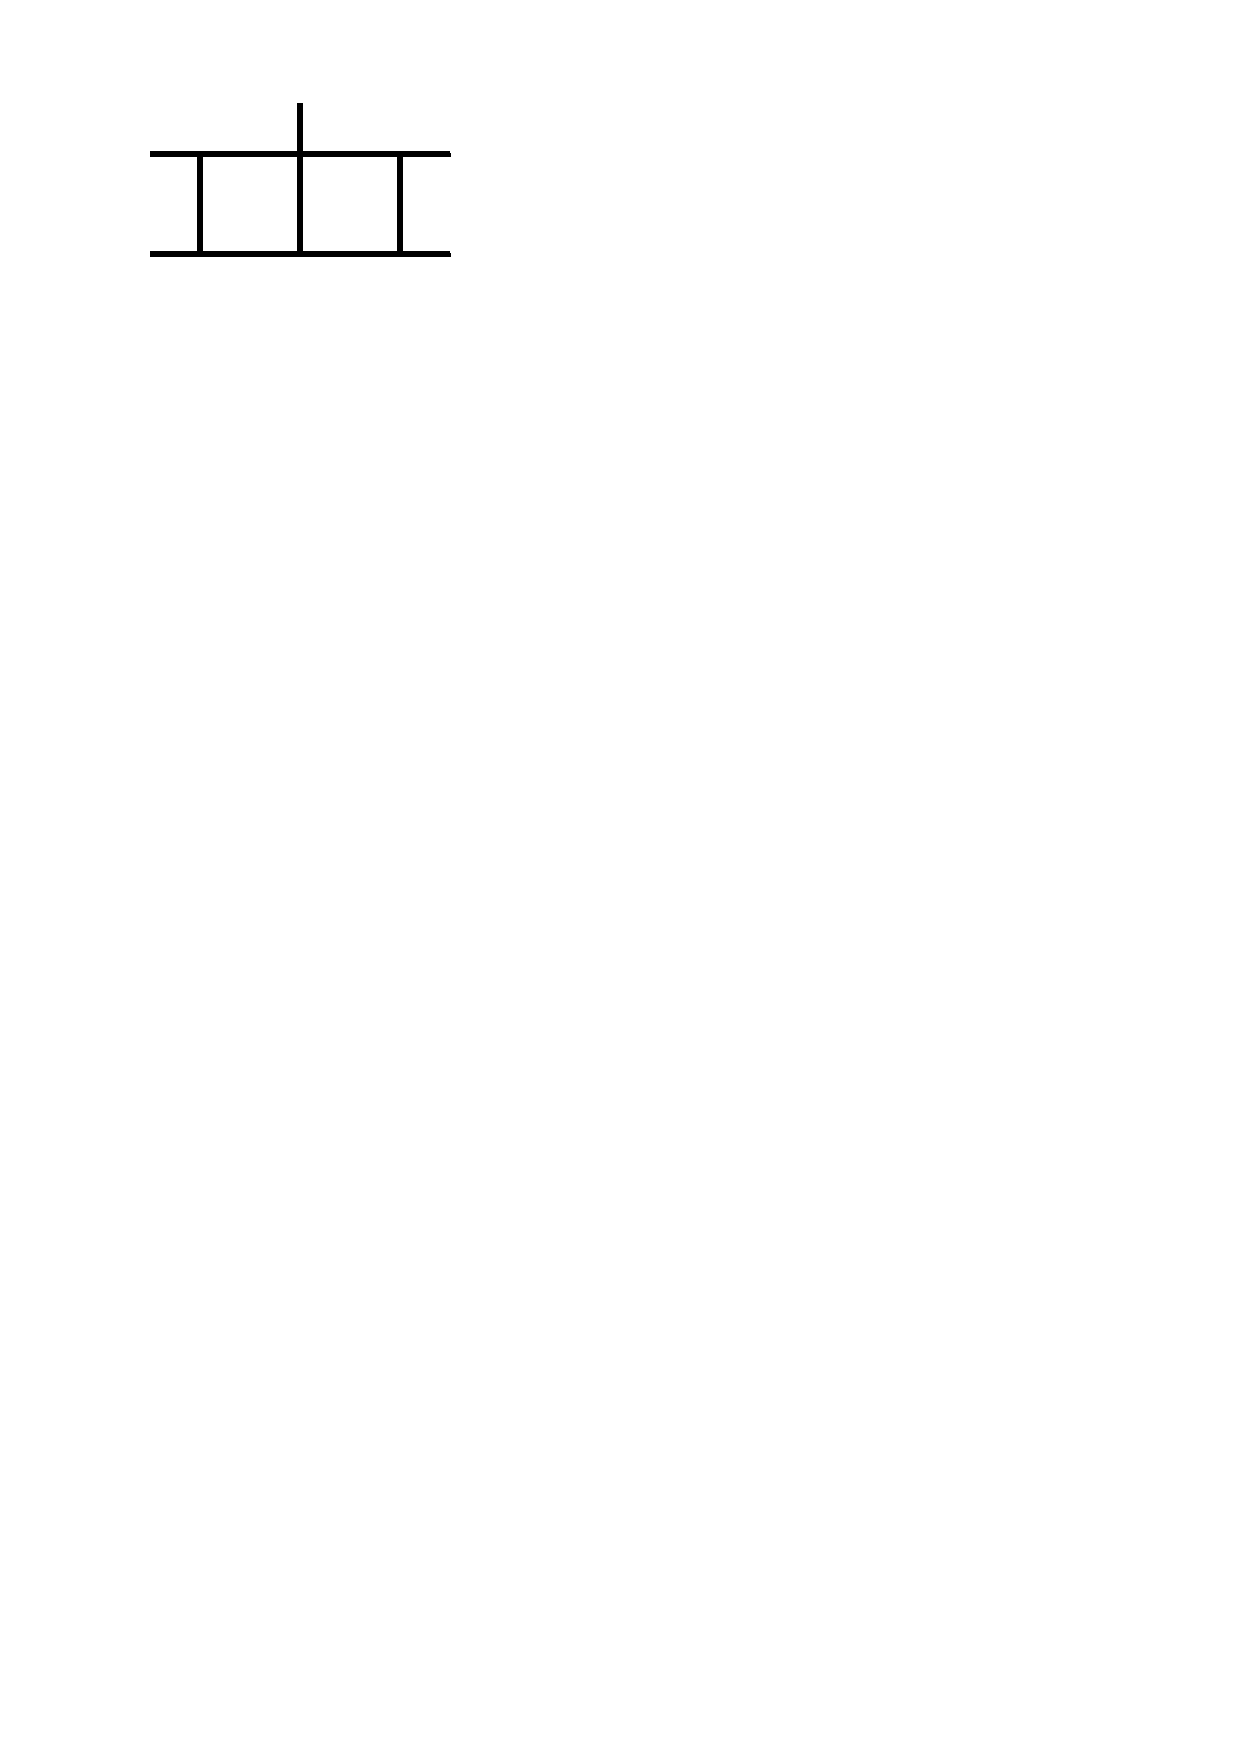
\includegraphics[scale=0.4]{figures/topologies/BoxBoxSG}};
      \node at
      (2.5,-2.0){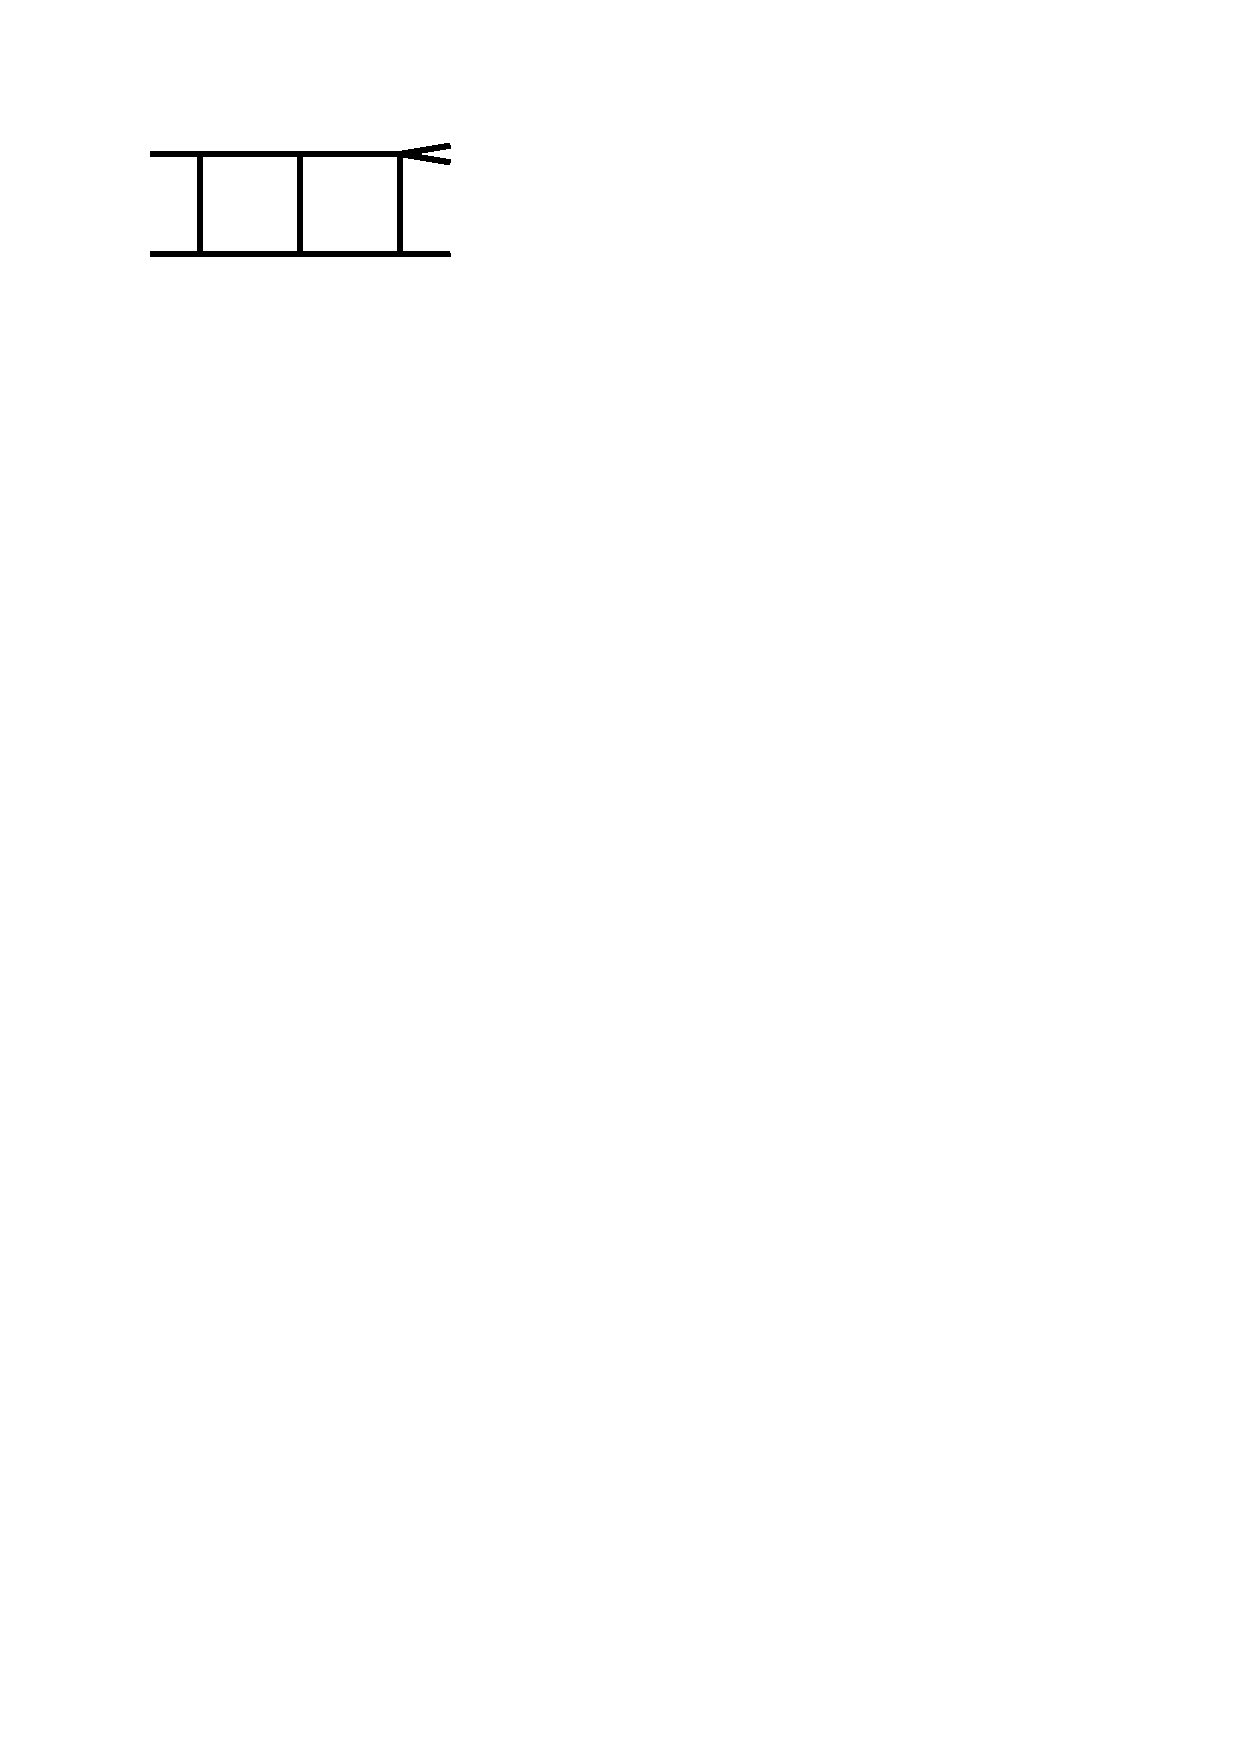
\includegraphics[scale=0.4]{figures/topologies/BoxBox}};
      \node at
      (5,-2.0){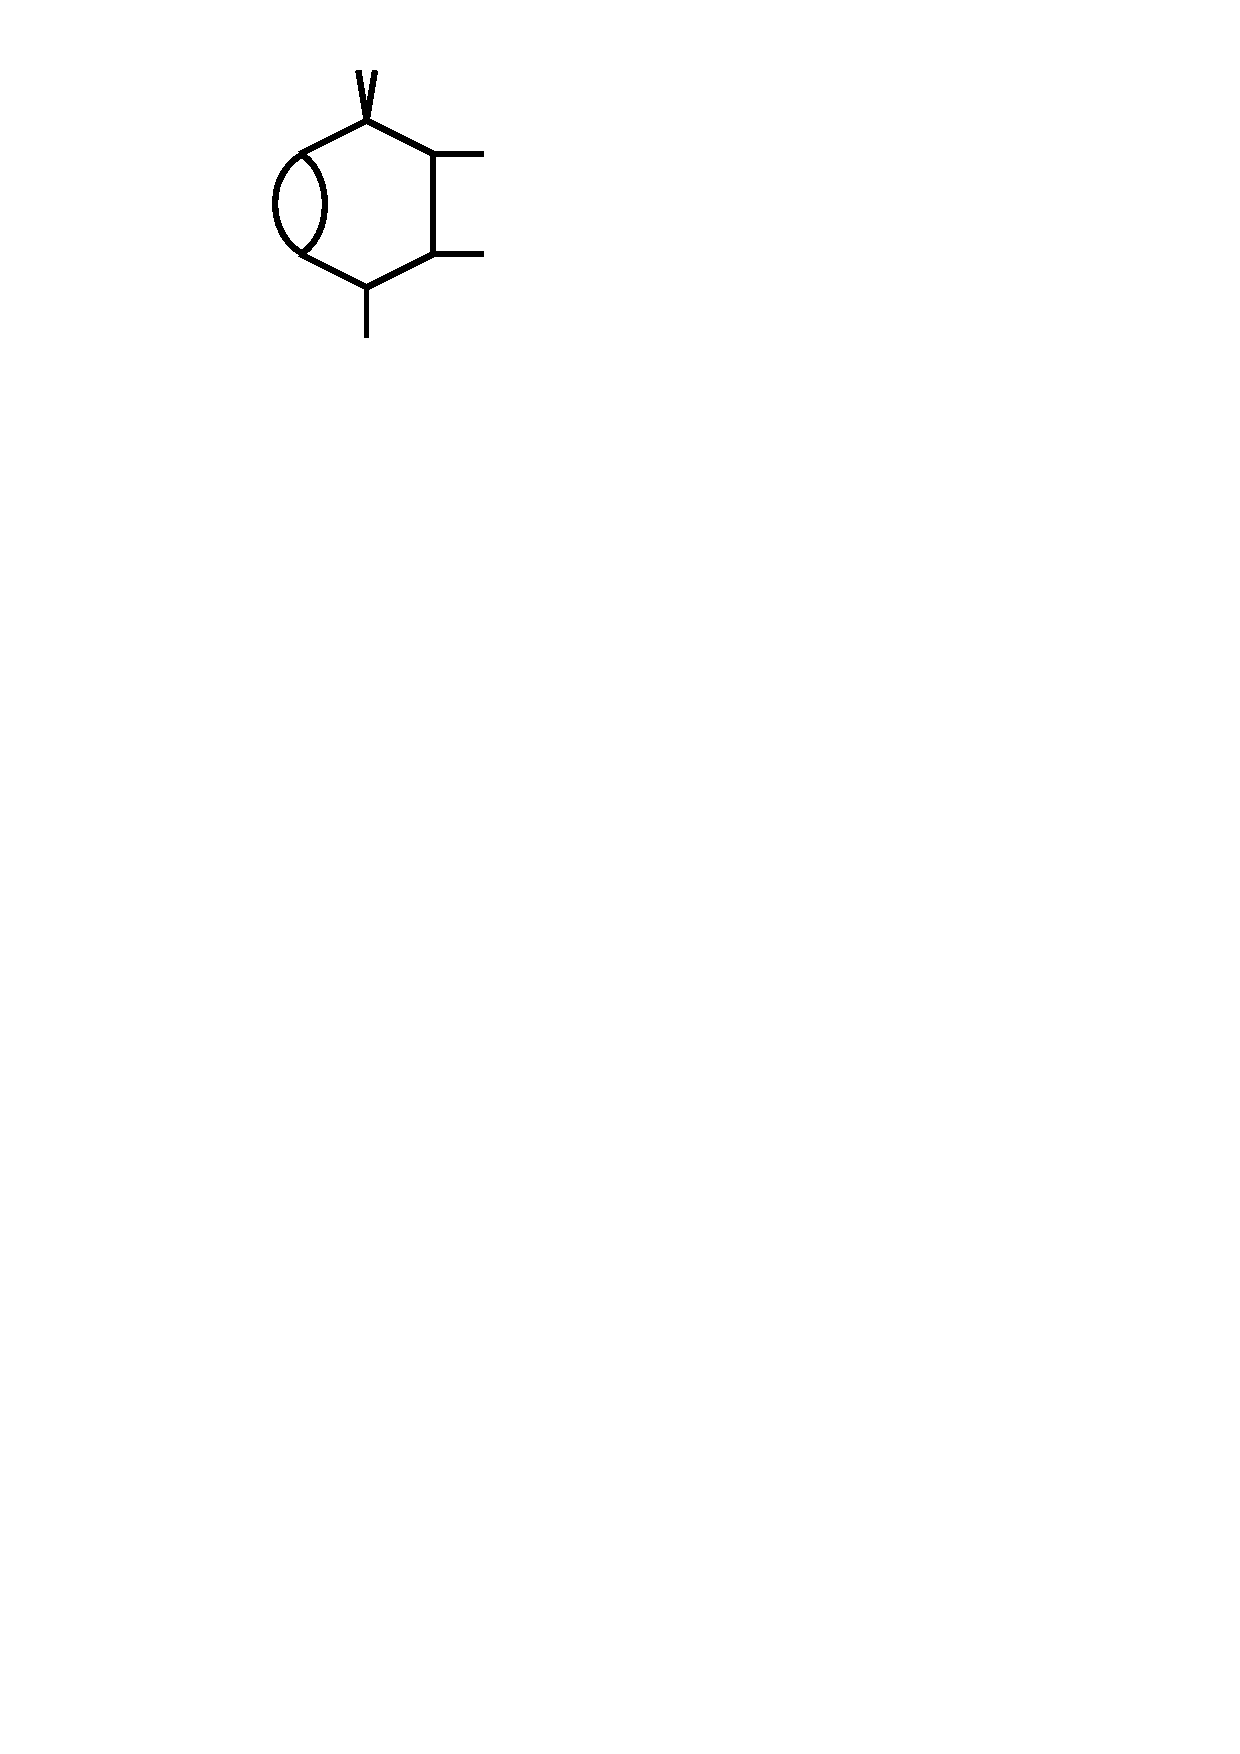
\includegraphics[scale=0.35]{figures/topologies/BubbleHexagonRed1}};
      \node at
      (7.5,-2.0){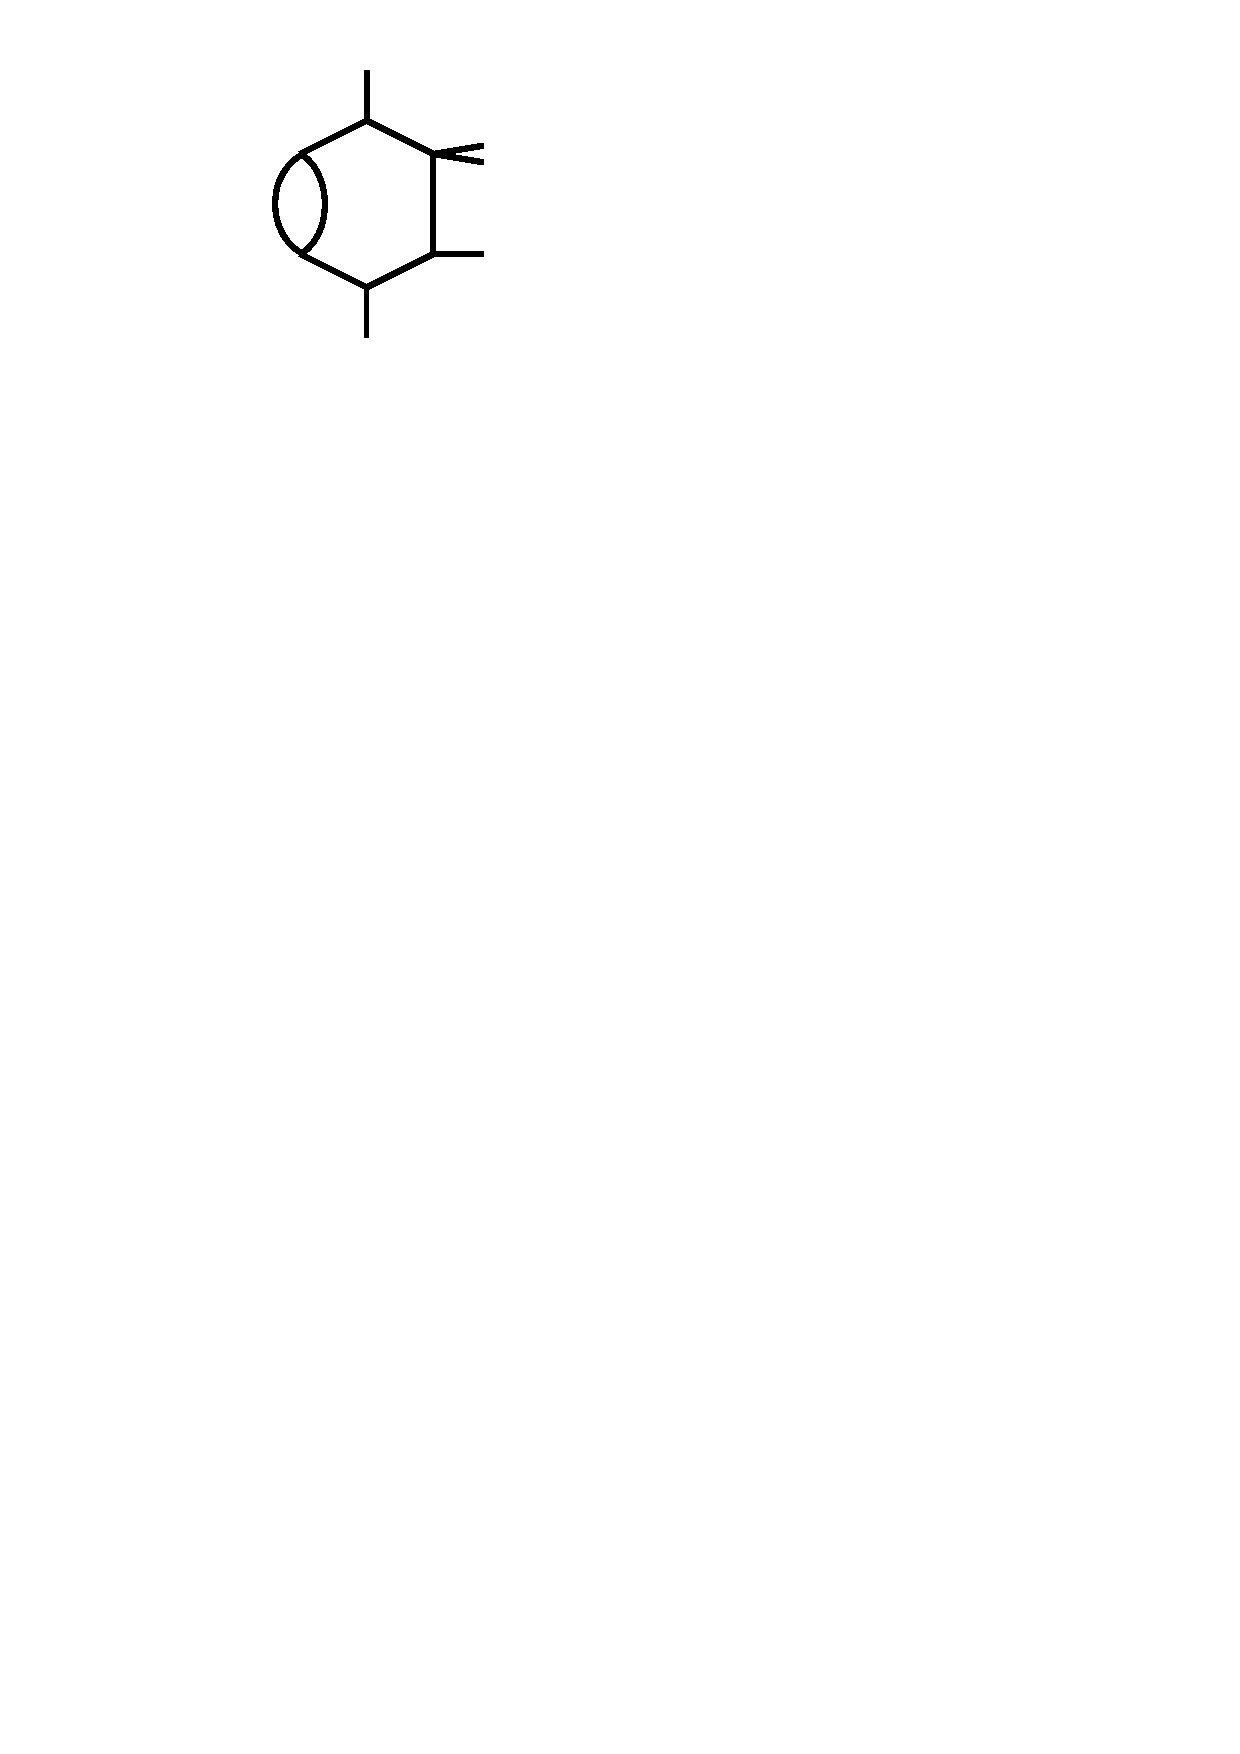
\includegraphics[scale=0.35]{figures/topologies/BubbleHexagonRed2}};
      \node at
      (10,-2.0){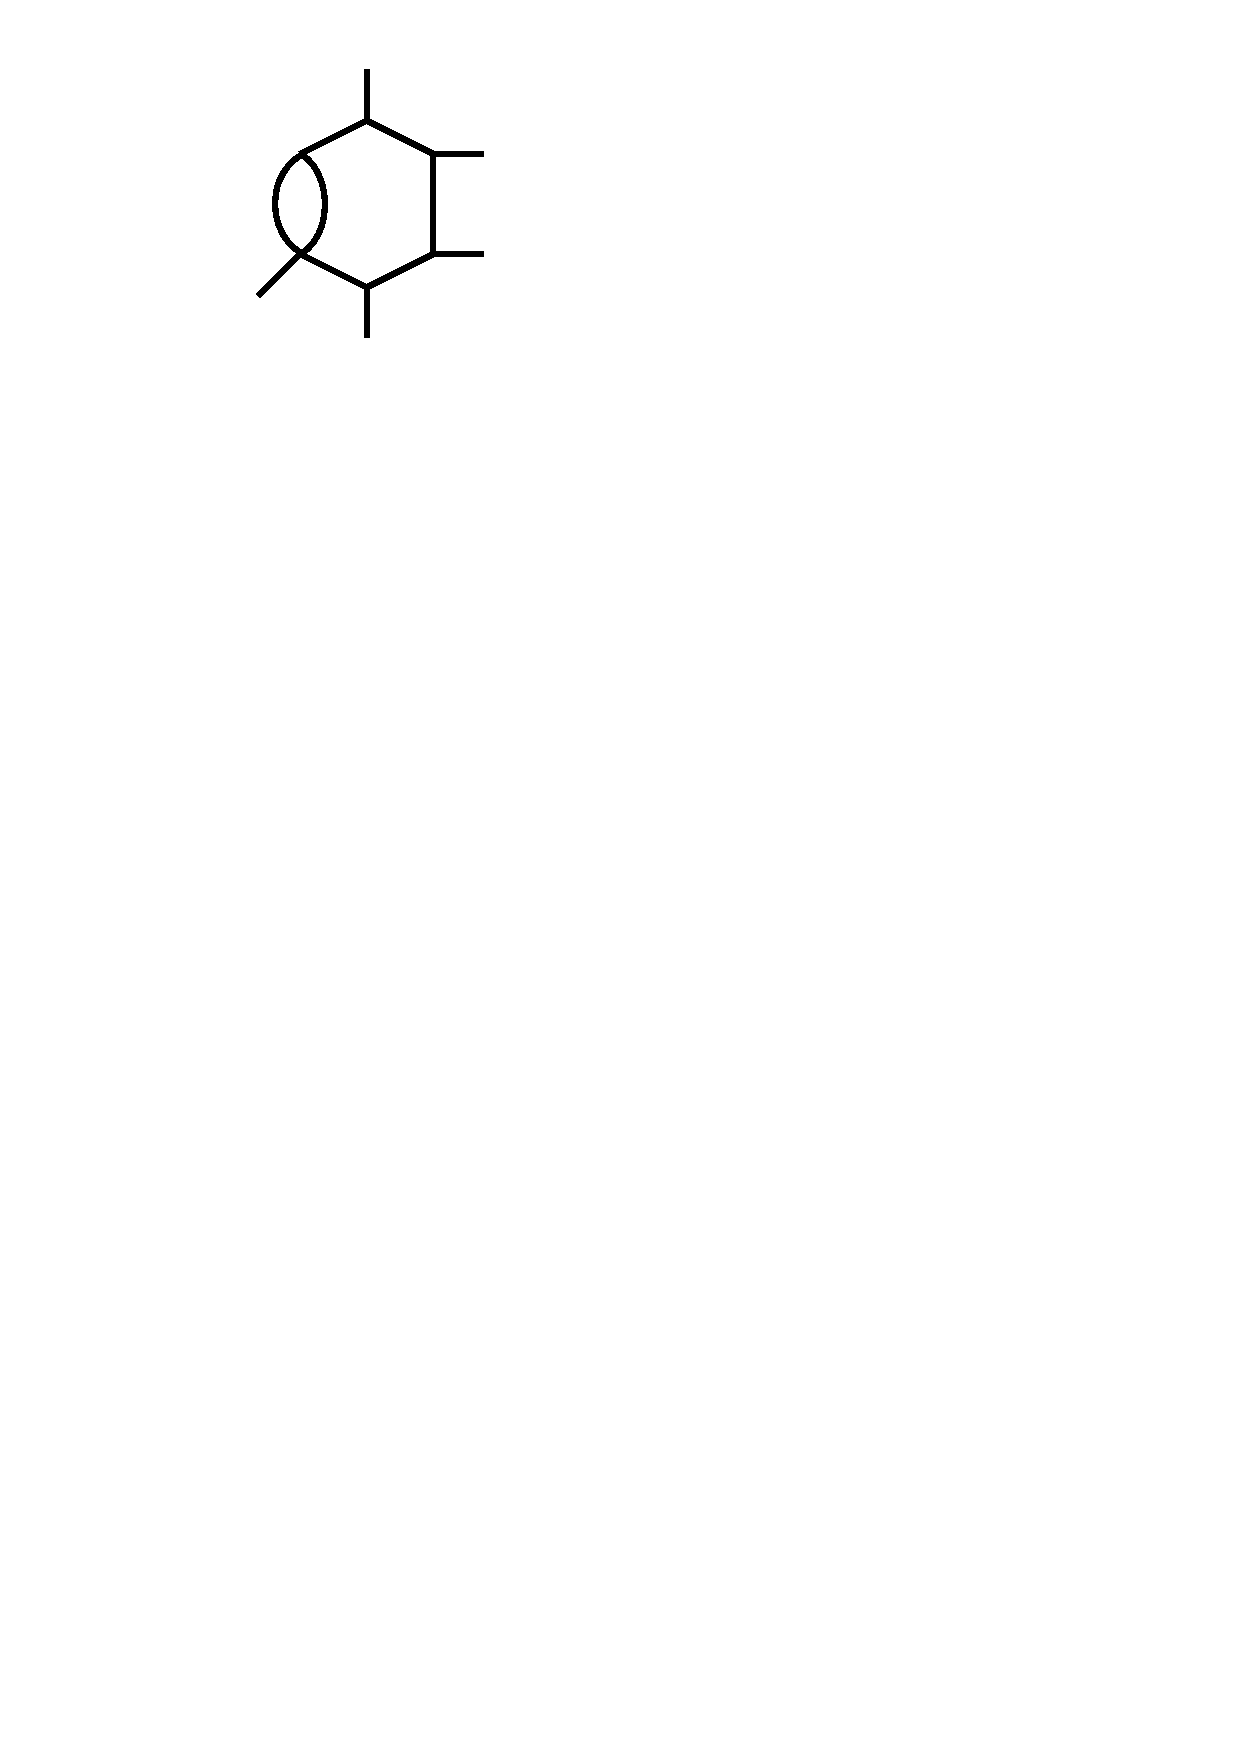
\includegraphics[scale=0.35]{figures/topologies/BubbleHexagonRed3}};
    %
      \node at
      (0,-3.6){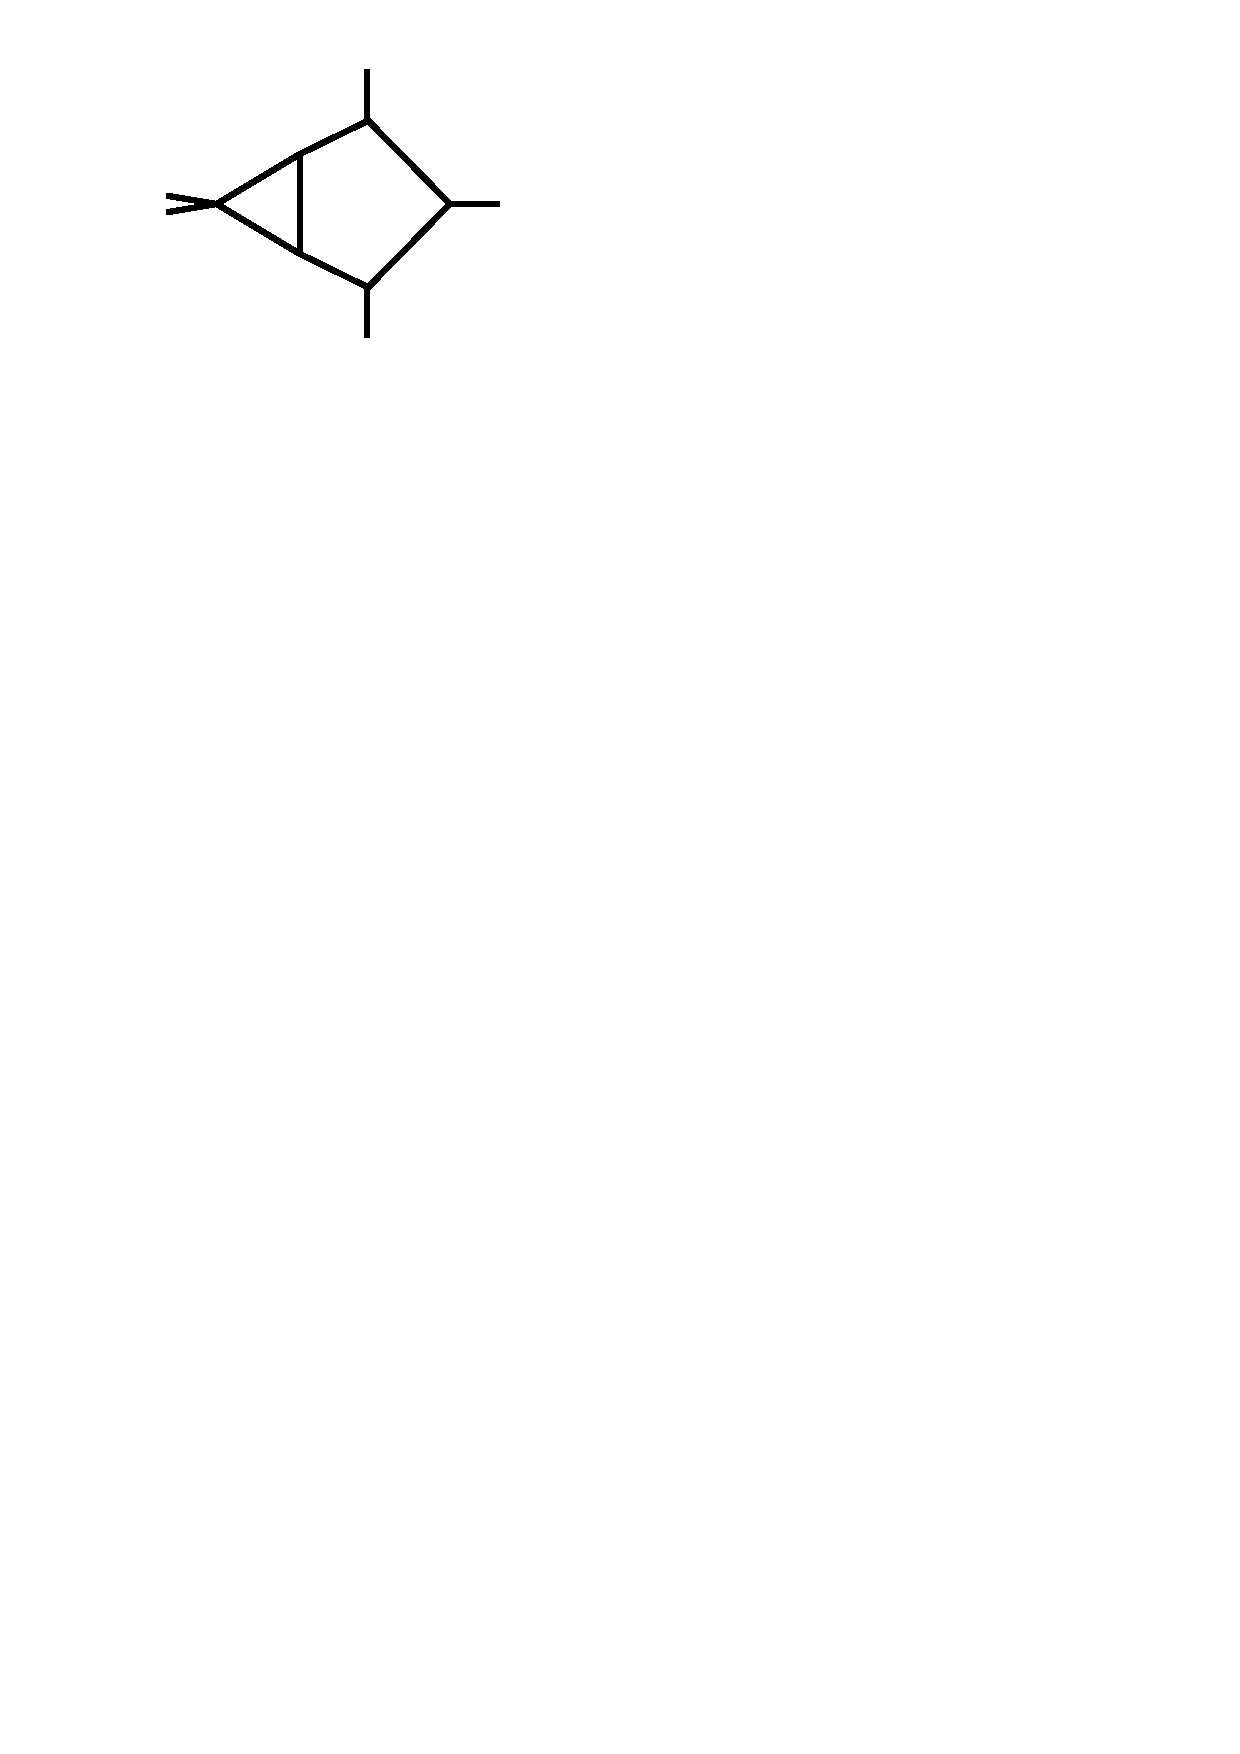
\includegraphics[scale=0.35]{figures/topologies/TrianglePentagonRed1}};
      \node at
      (2.5,-3.6){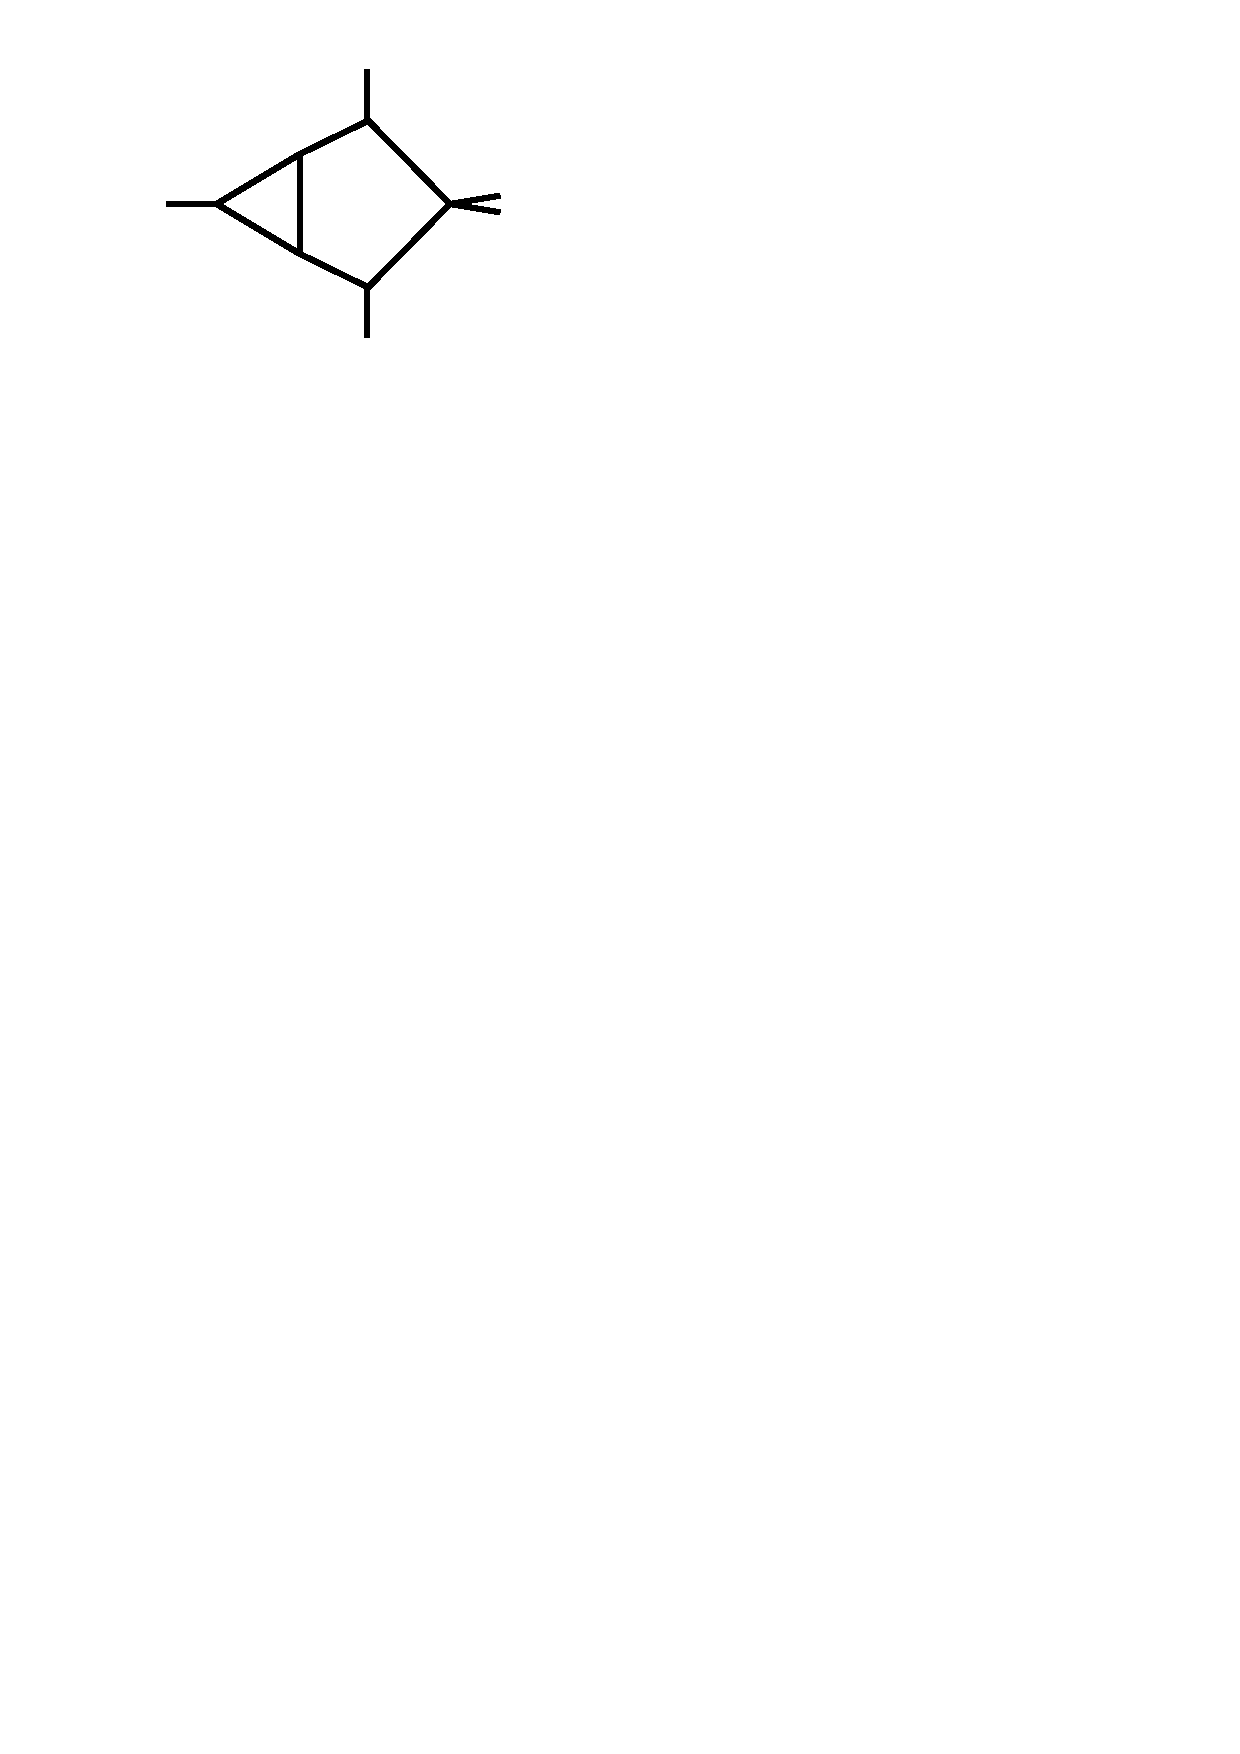
\includegraphics[scale=0.35]{figures/topologies/TrianglePentagonRed2}};
      \node at
      (5,-3.6){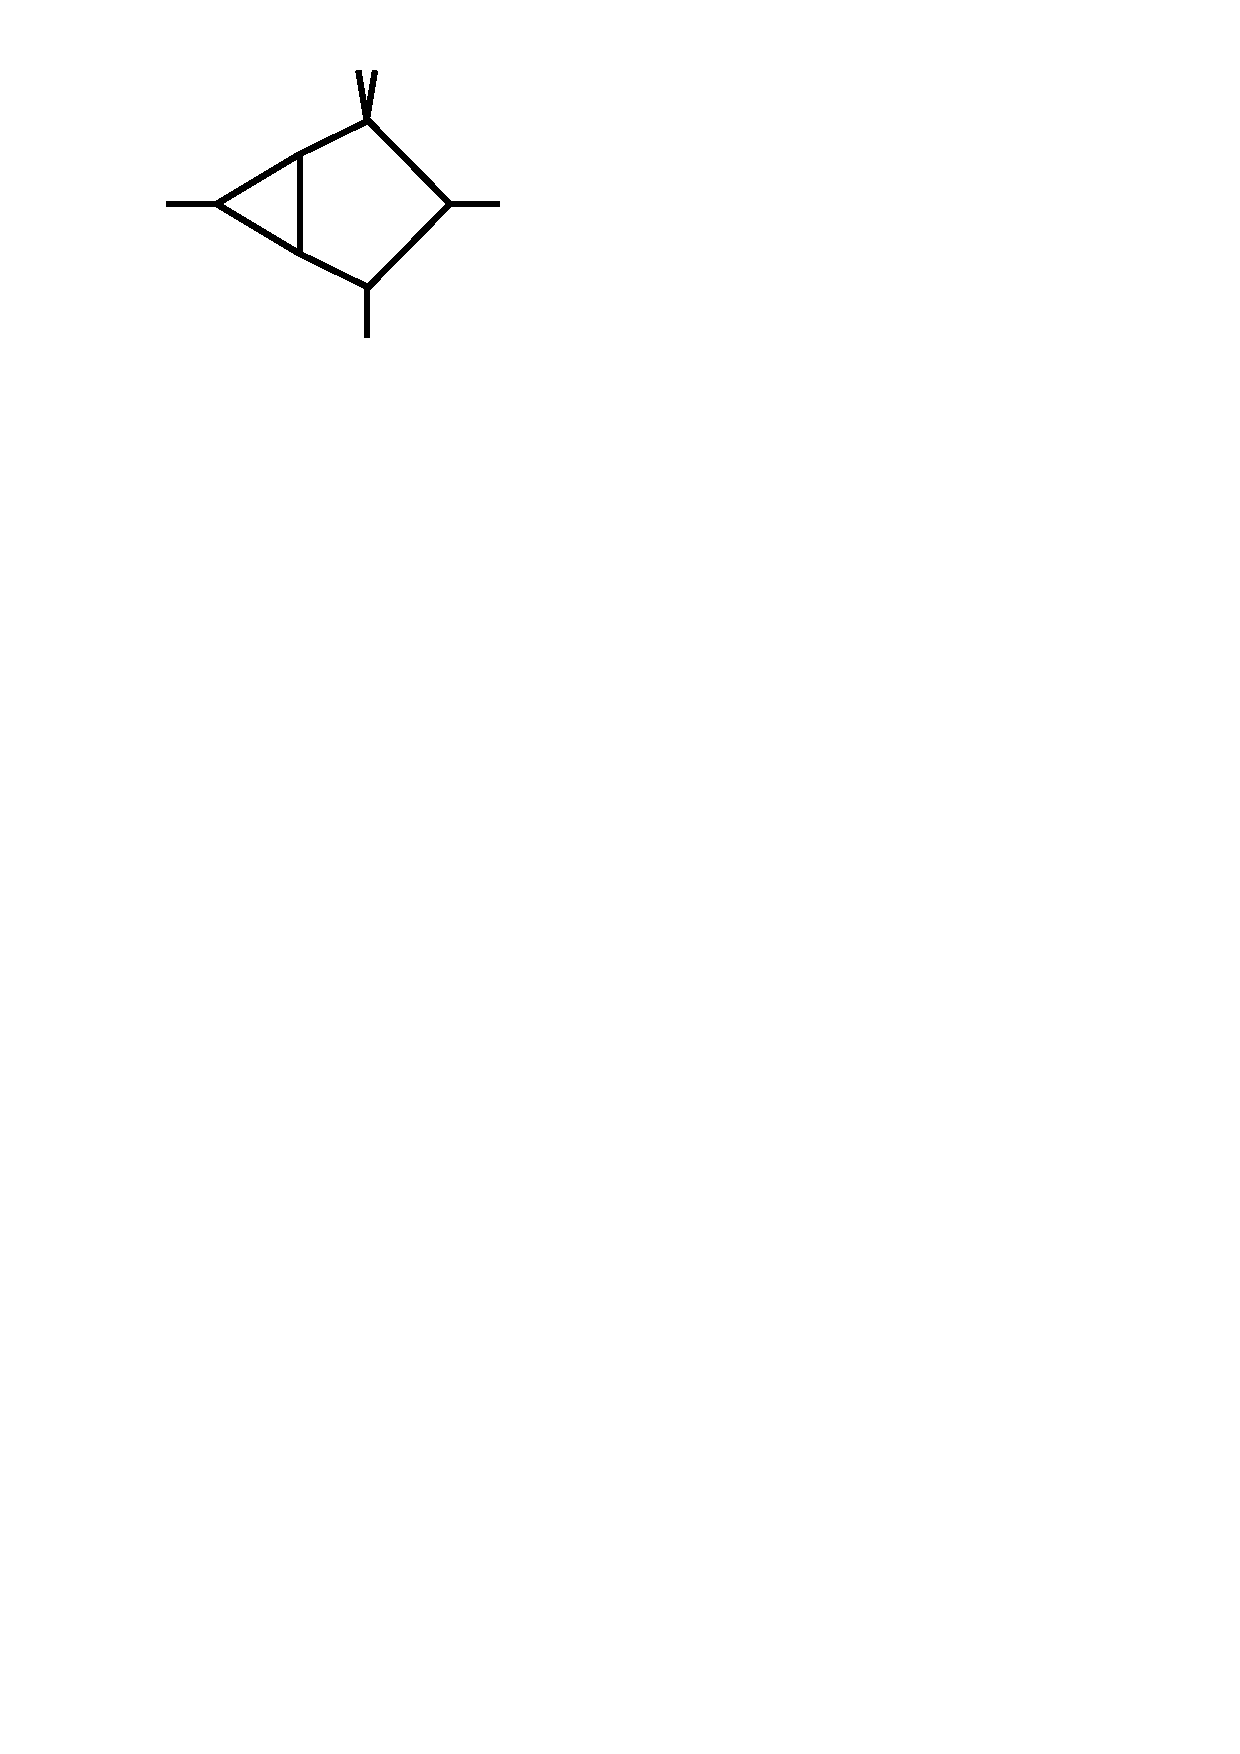
\includegraphics[scale=0.35]{figures/topologies/TrianglePentagonRed3}};
      \node at
      (7.5,-3.6){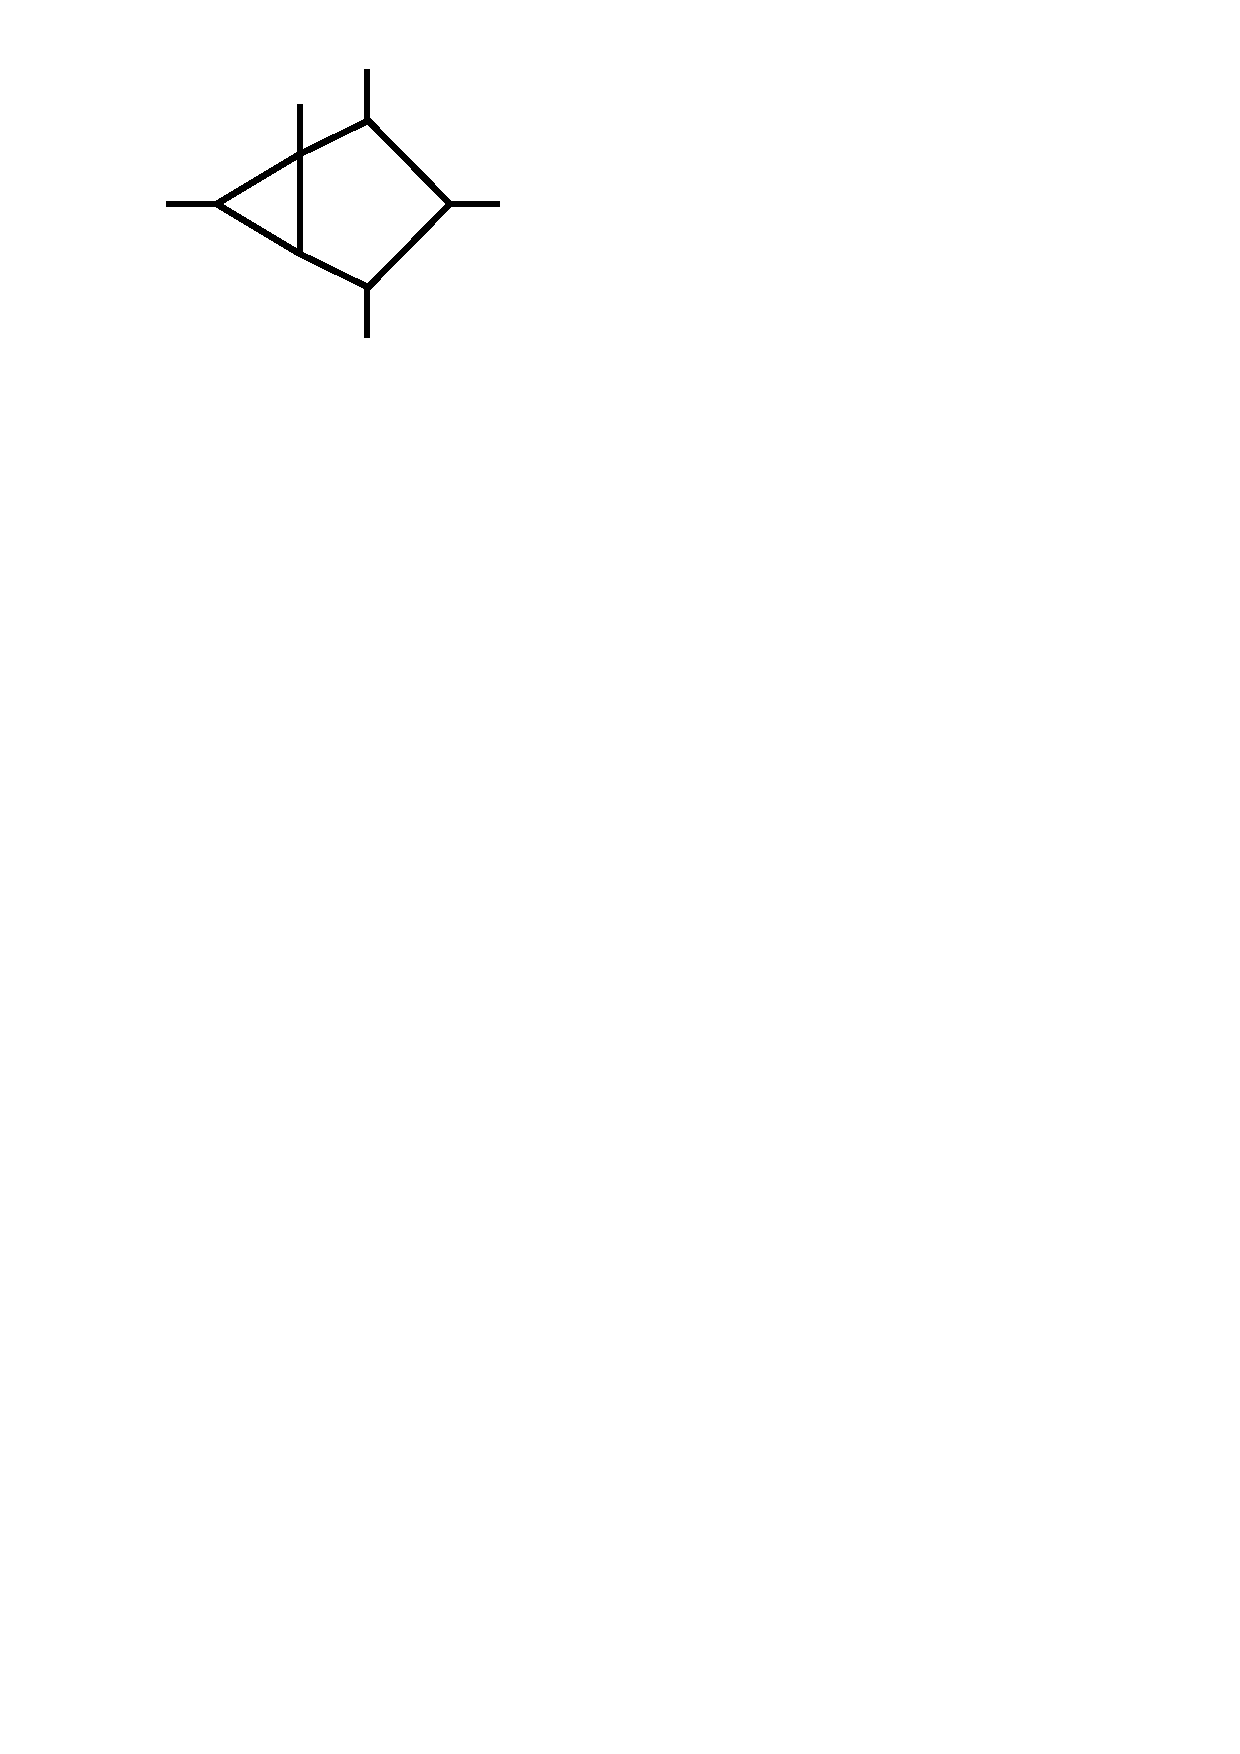
\includegraphics[scale=0.35]{figures/topologies/TrianglePentagonRed4}};
      \node at
      (10,-3.6){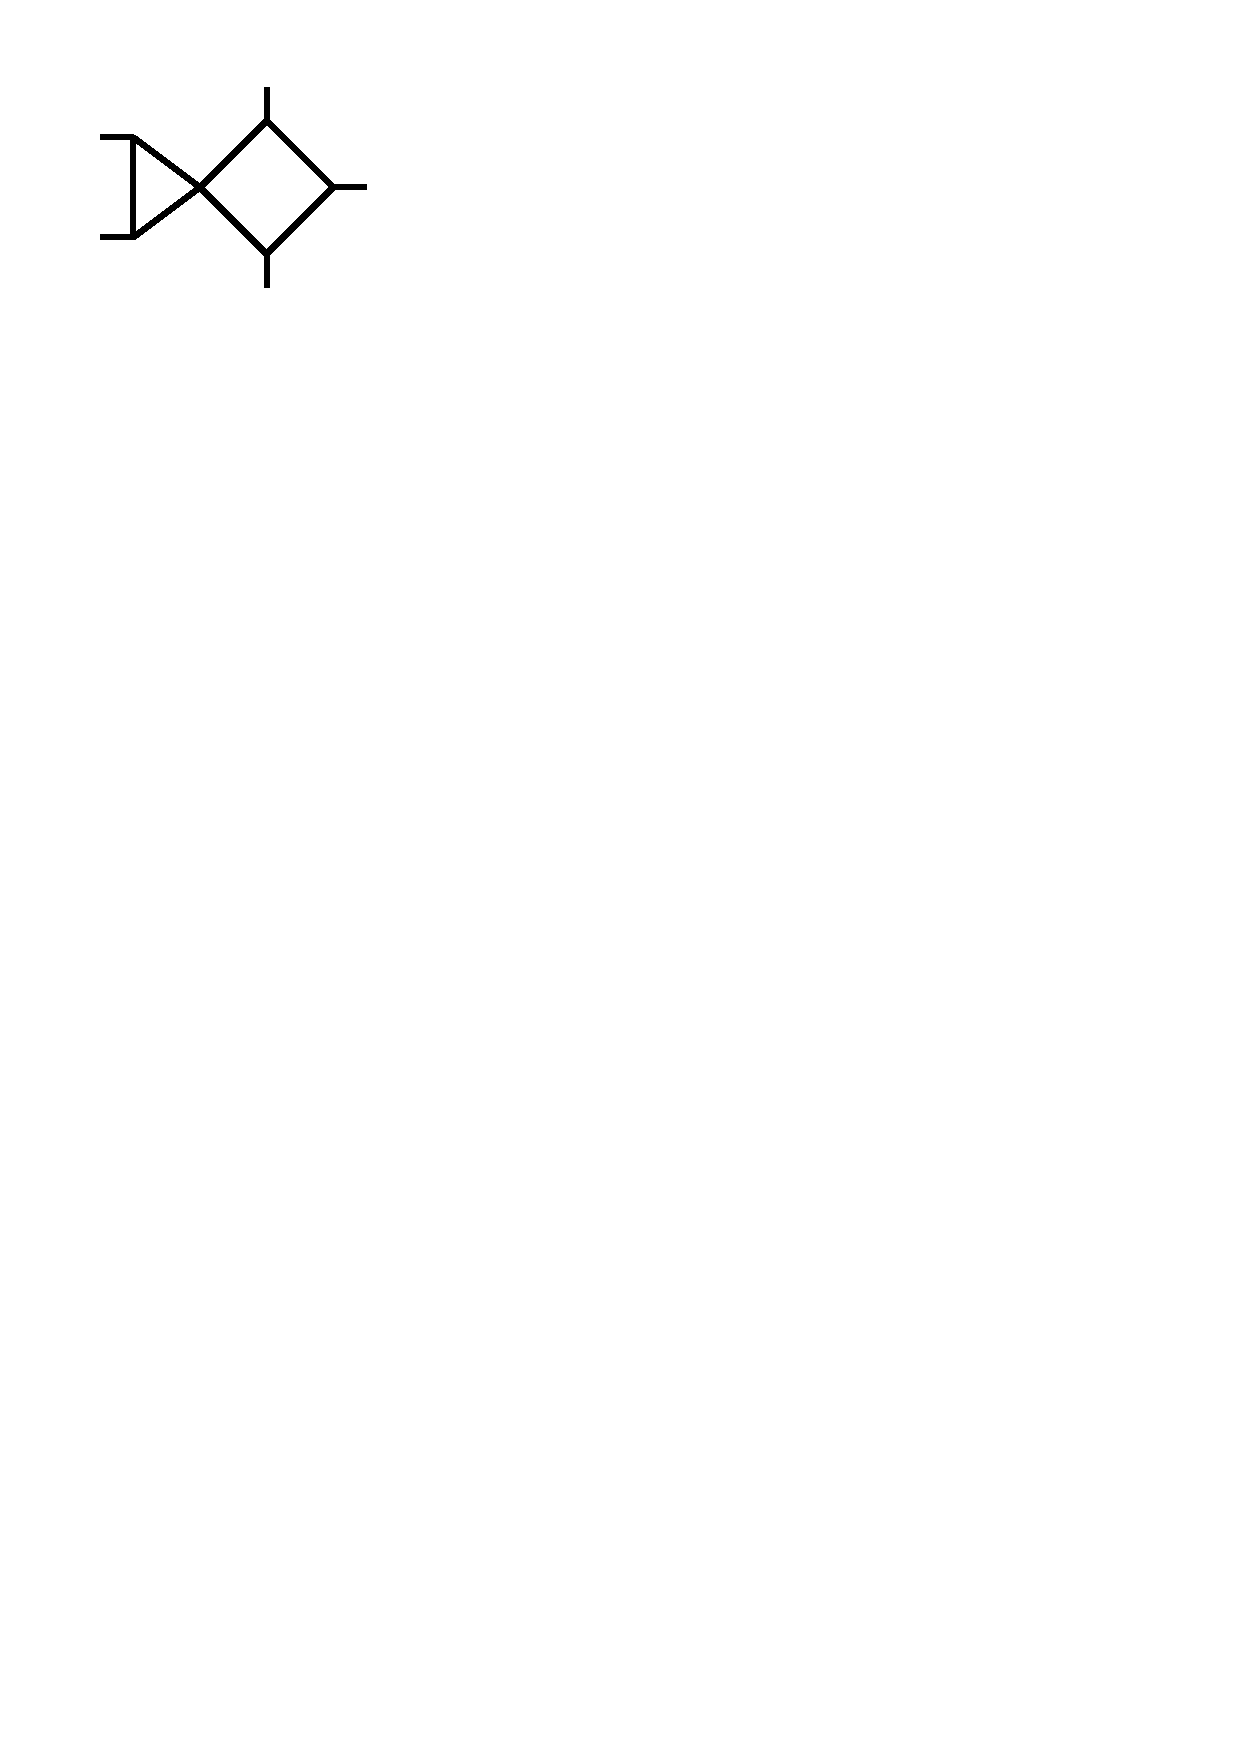
\includegraphics[scale=0.4]{figures/topologies/BoxTriangle1LS}};
    % Level 3
      \node at
      (0,-5.5){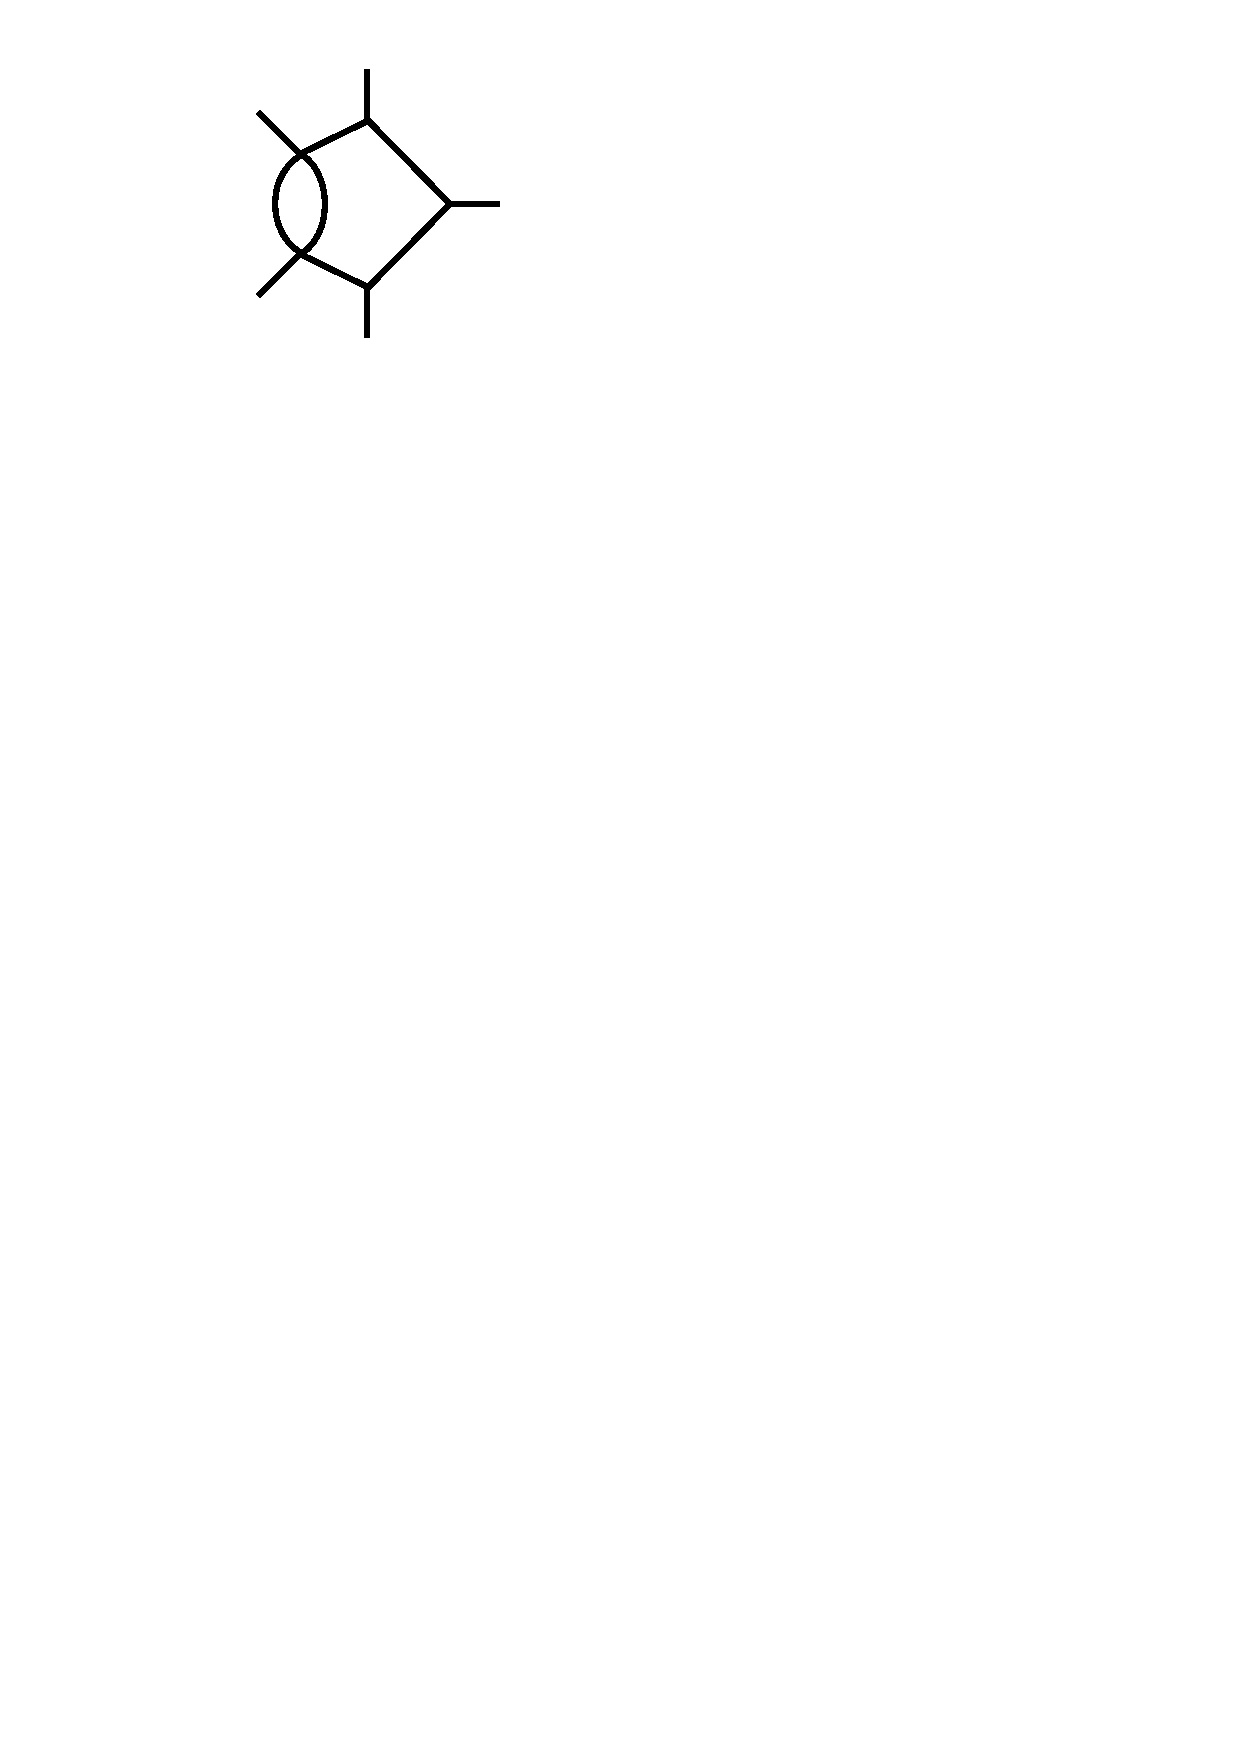
\includegraphics[scale=0.35]{figures/topologies/BubblePentagonG}};
      \node at
      (2,-5.5){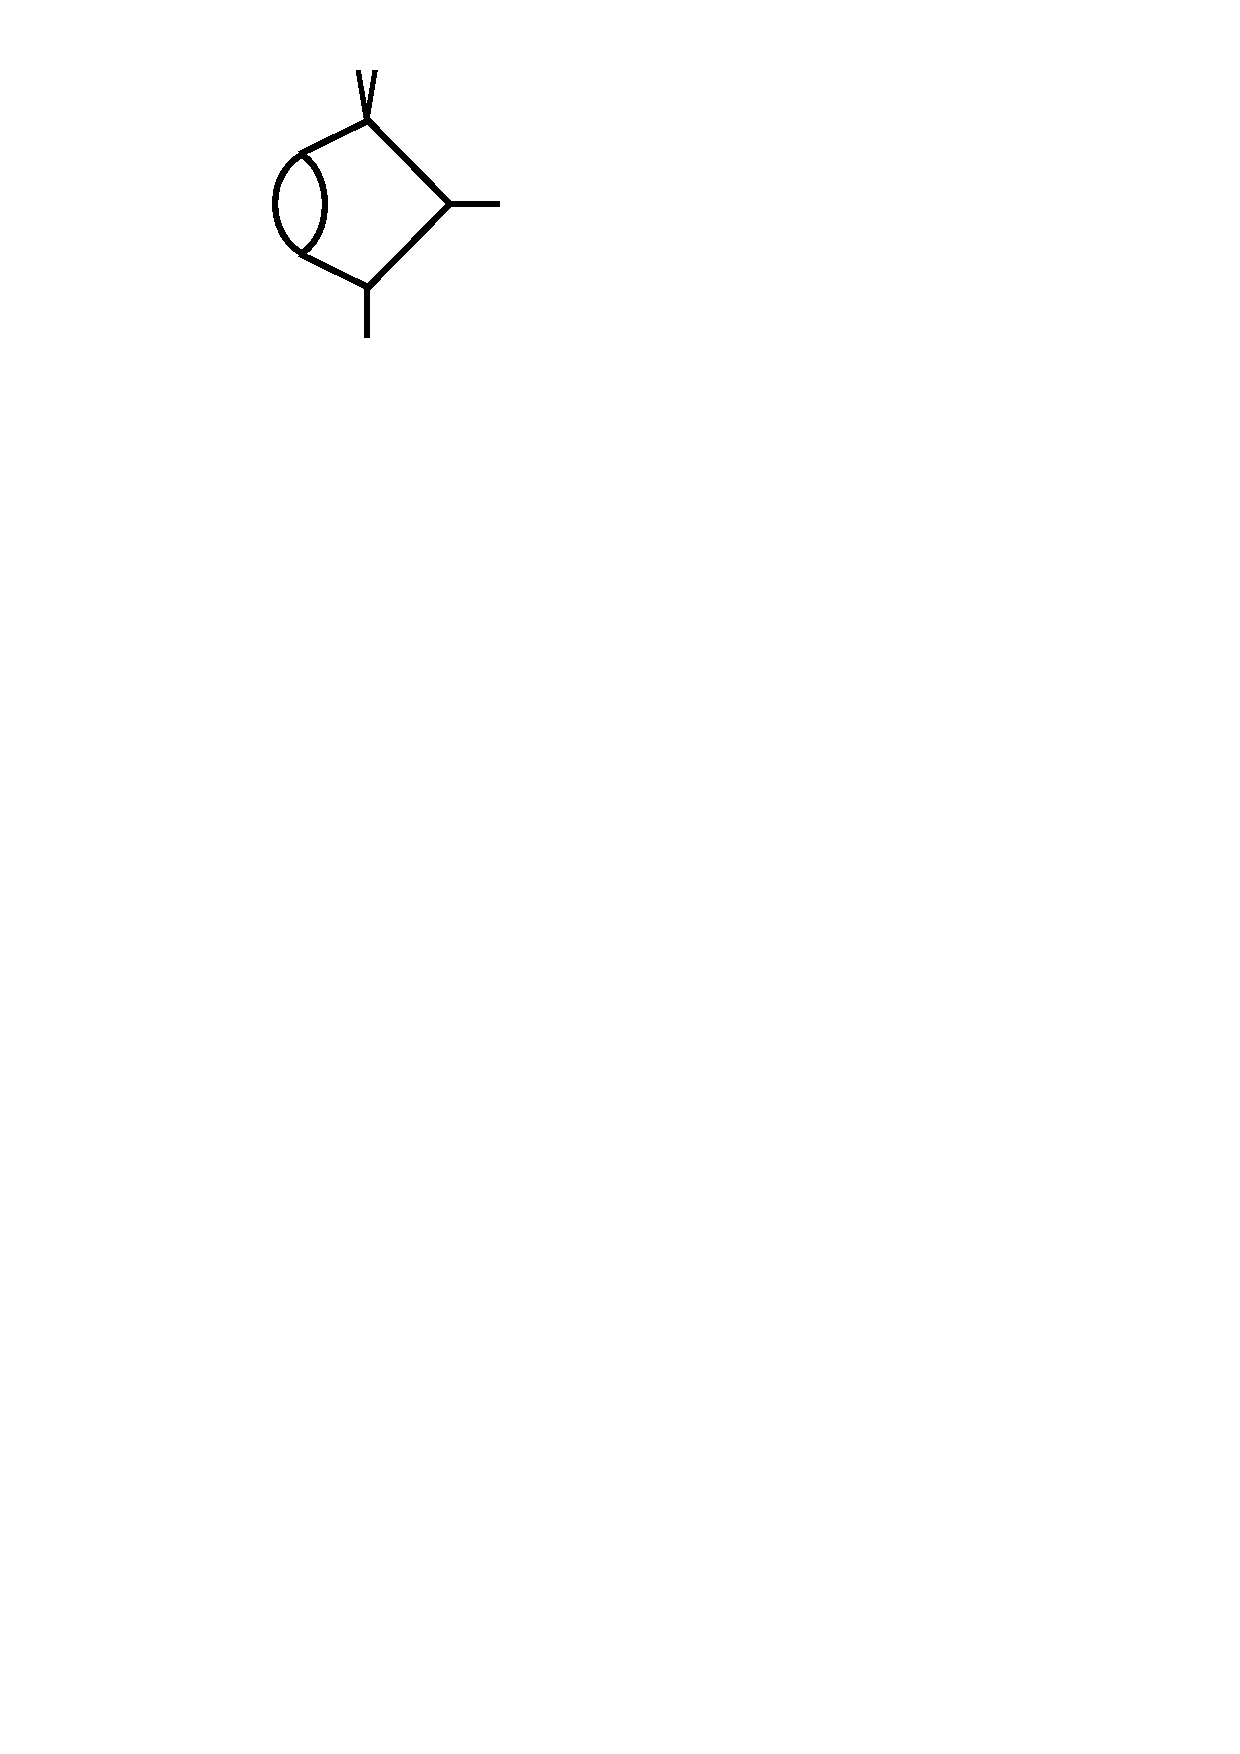
\includegraphics[scale=0.35]{figures/topologies/BubblePentagonRed1}};
      \node at
      (4,-5.5){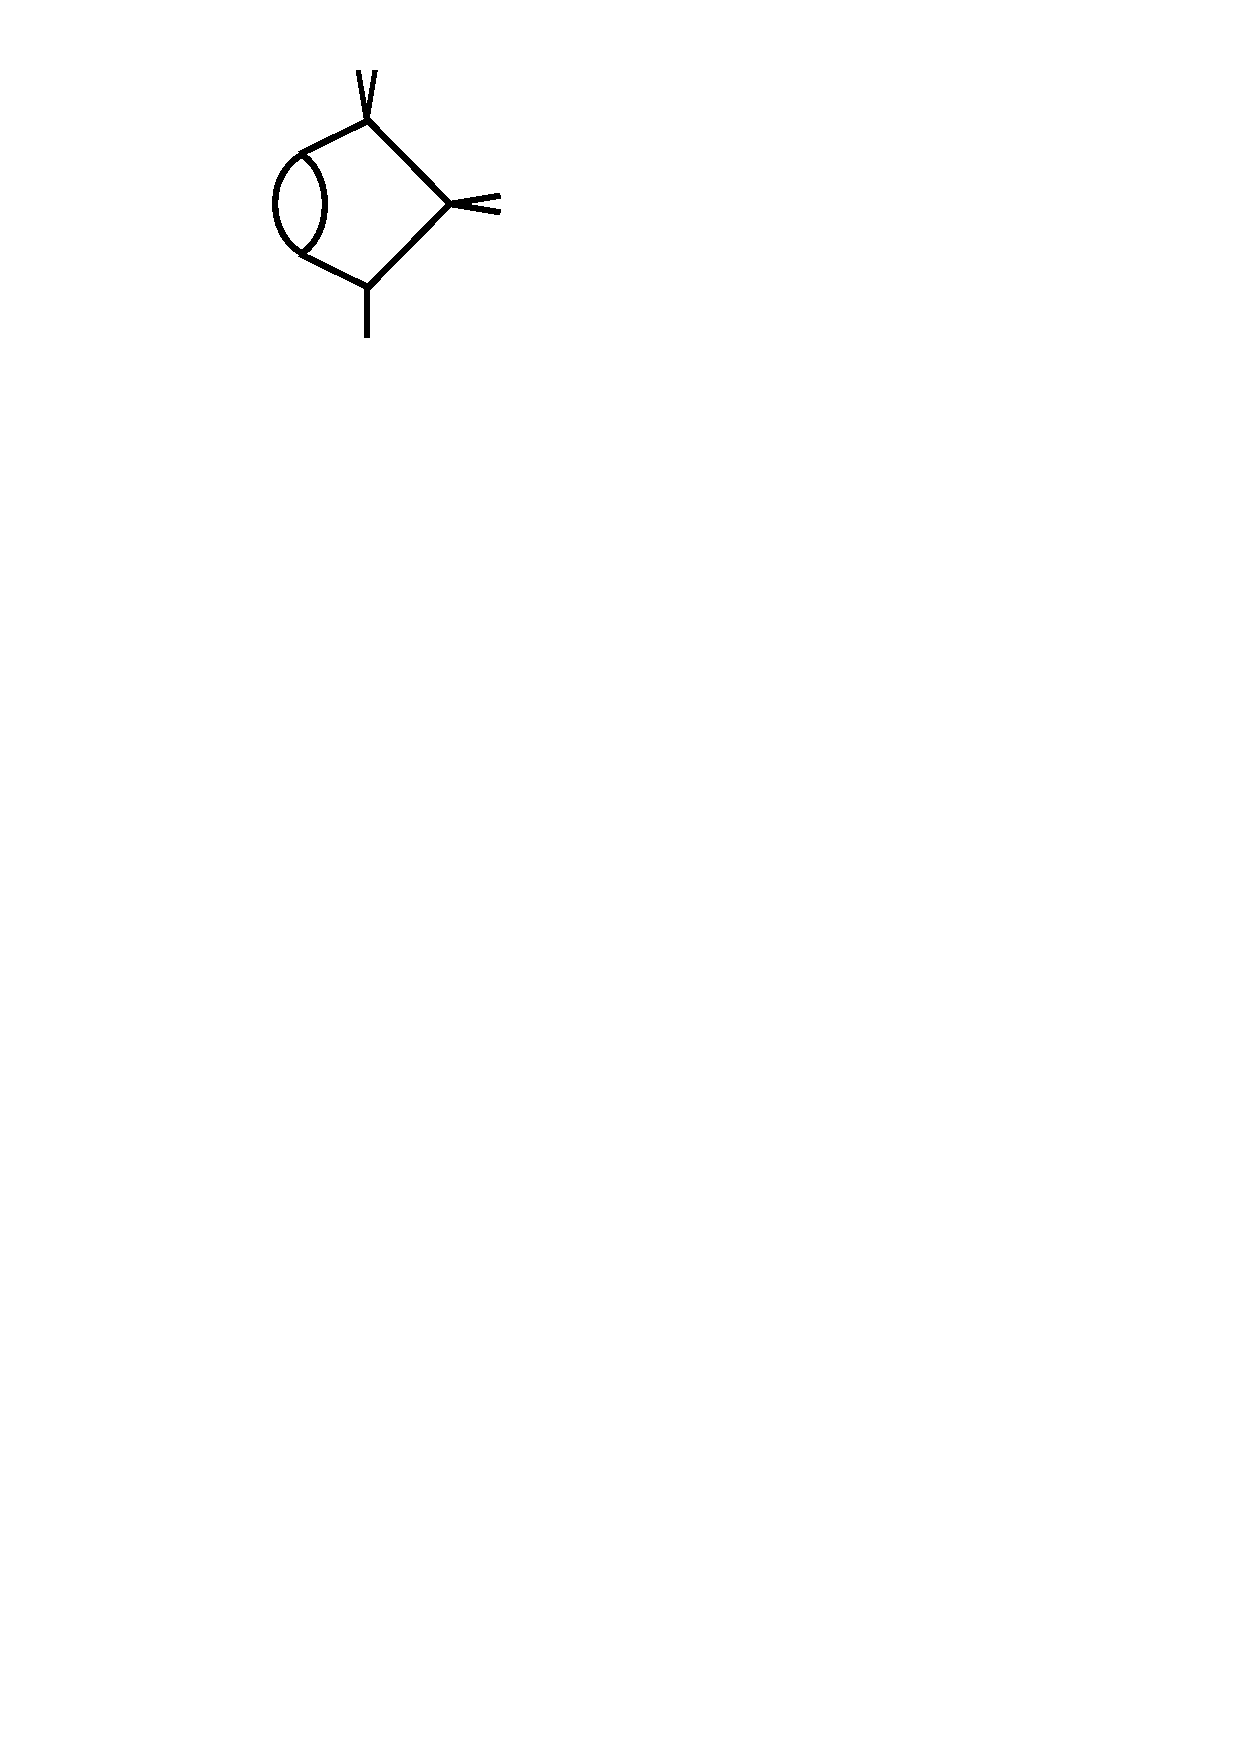
\includegraphics[scale=0.35]{figures/topologies/BubblePentagonRed2}};
      \node at
      (6,-5.5){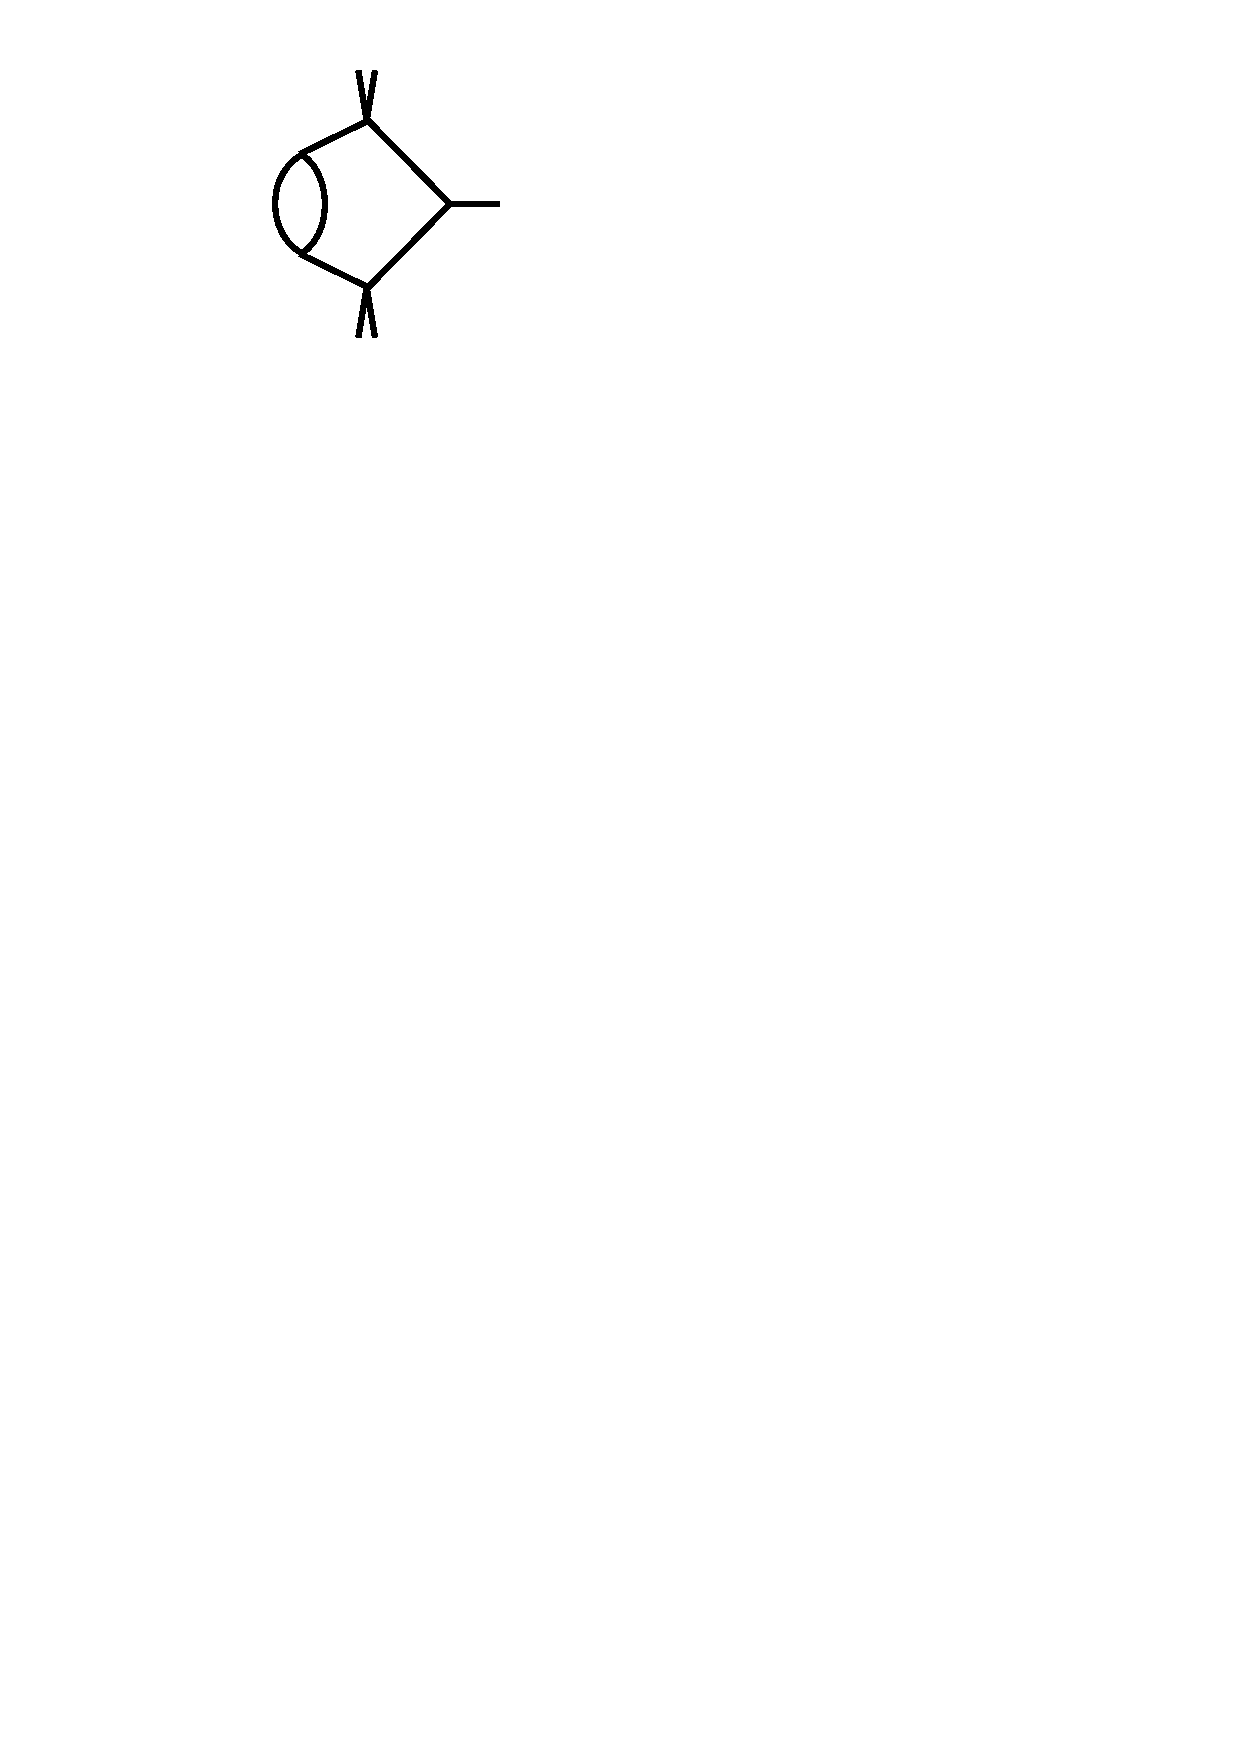
\includegraphics[scale=0.35]{figures/topologies/BubblePentagonRed3}};
      \node at
      (8,-5.5){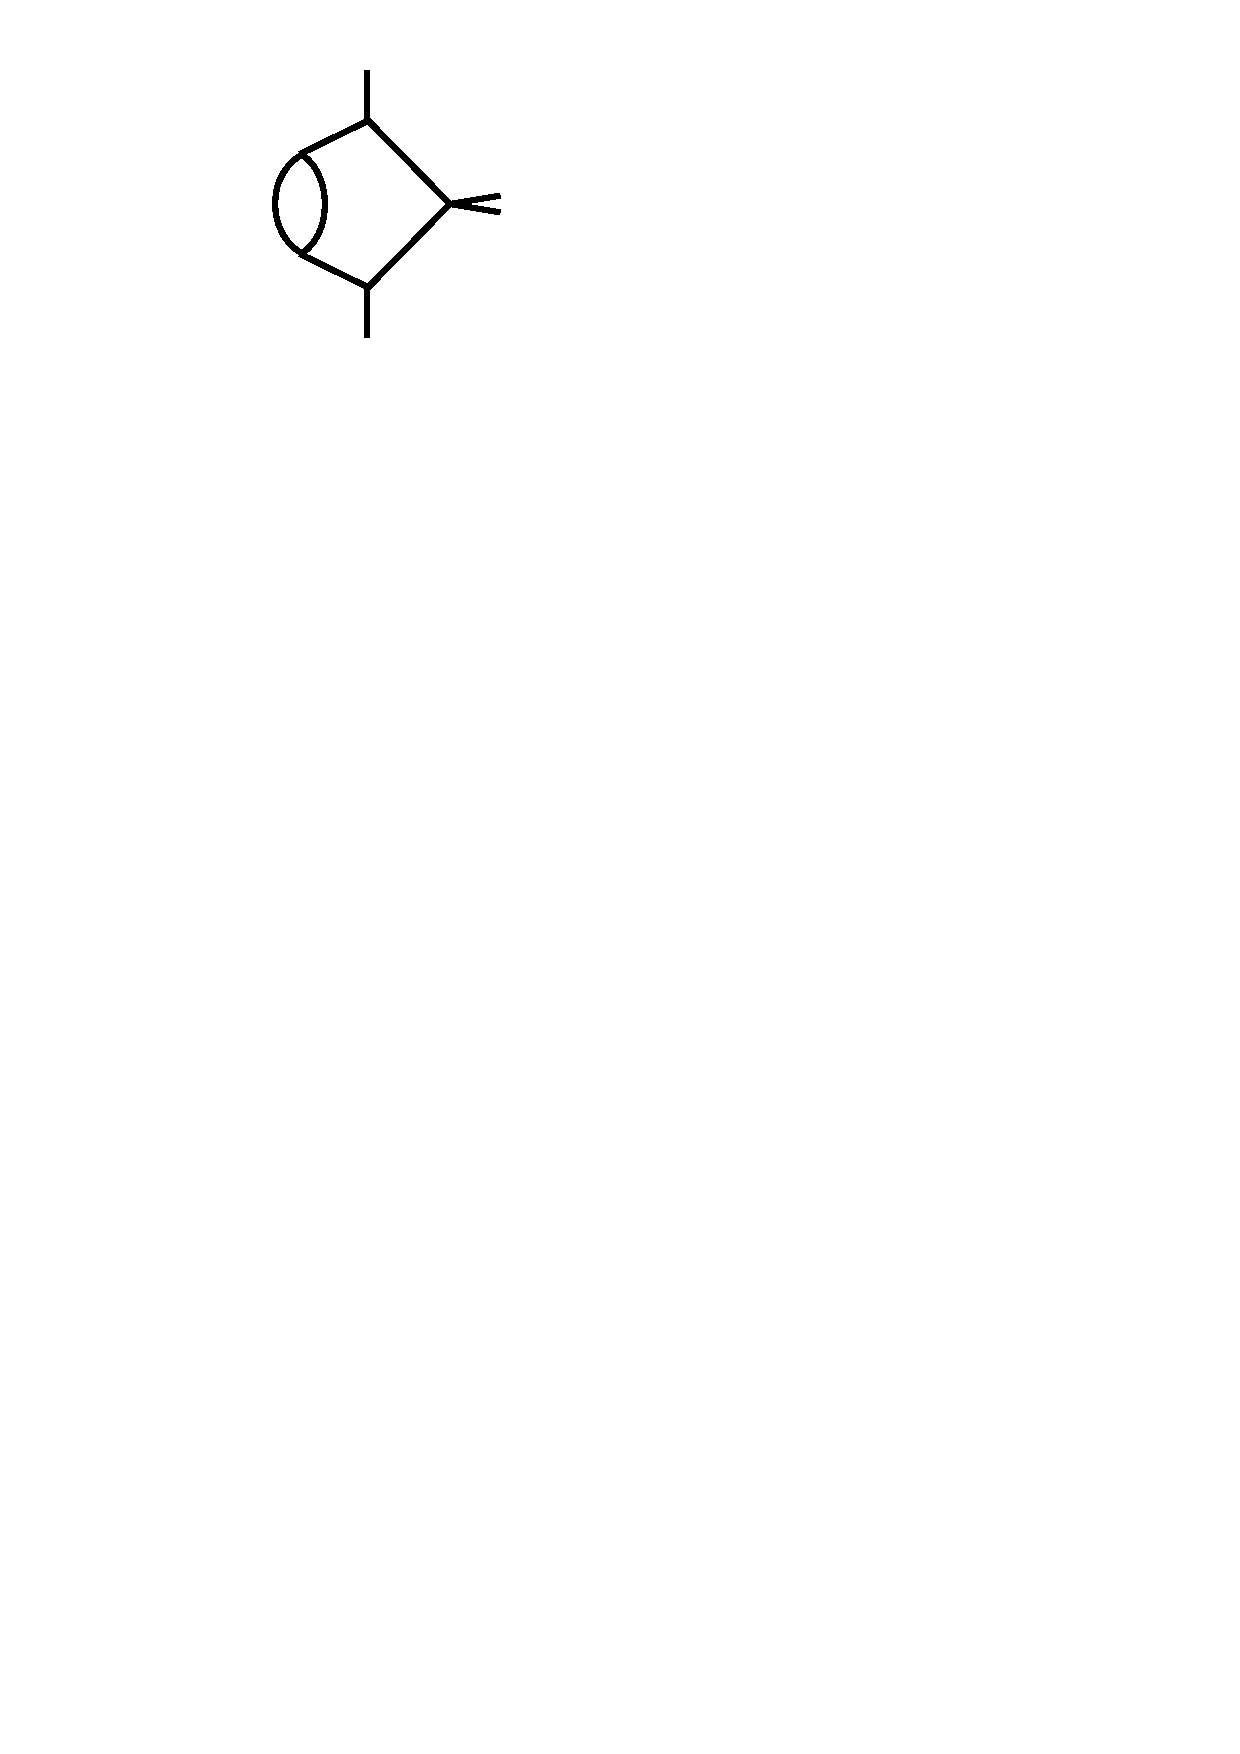
\includegraphics[scale=0.35]{figures/topologies/BubblePentagonRed4}};
      \node at
      (10,-5.5){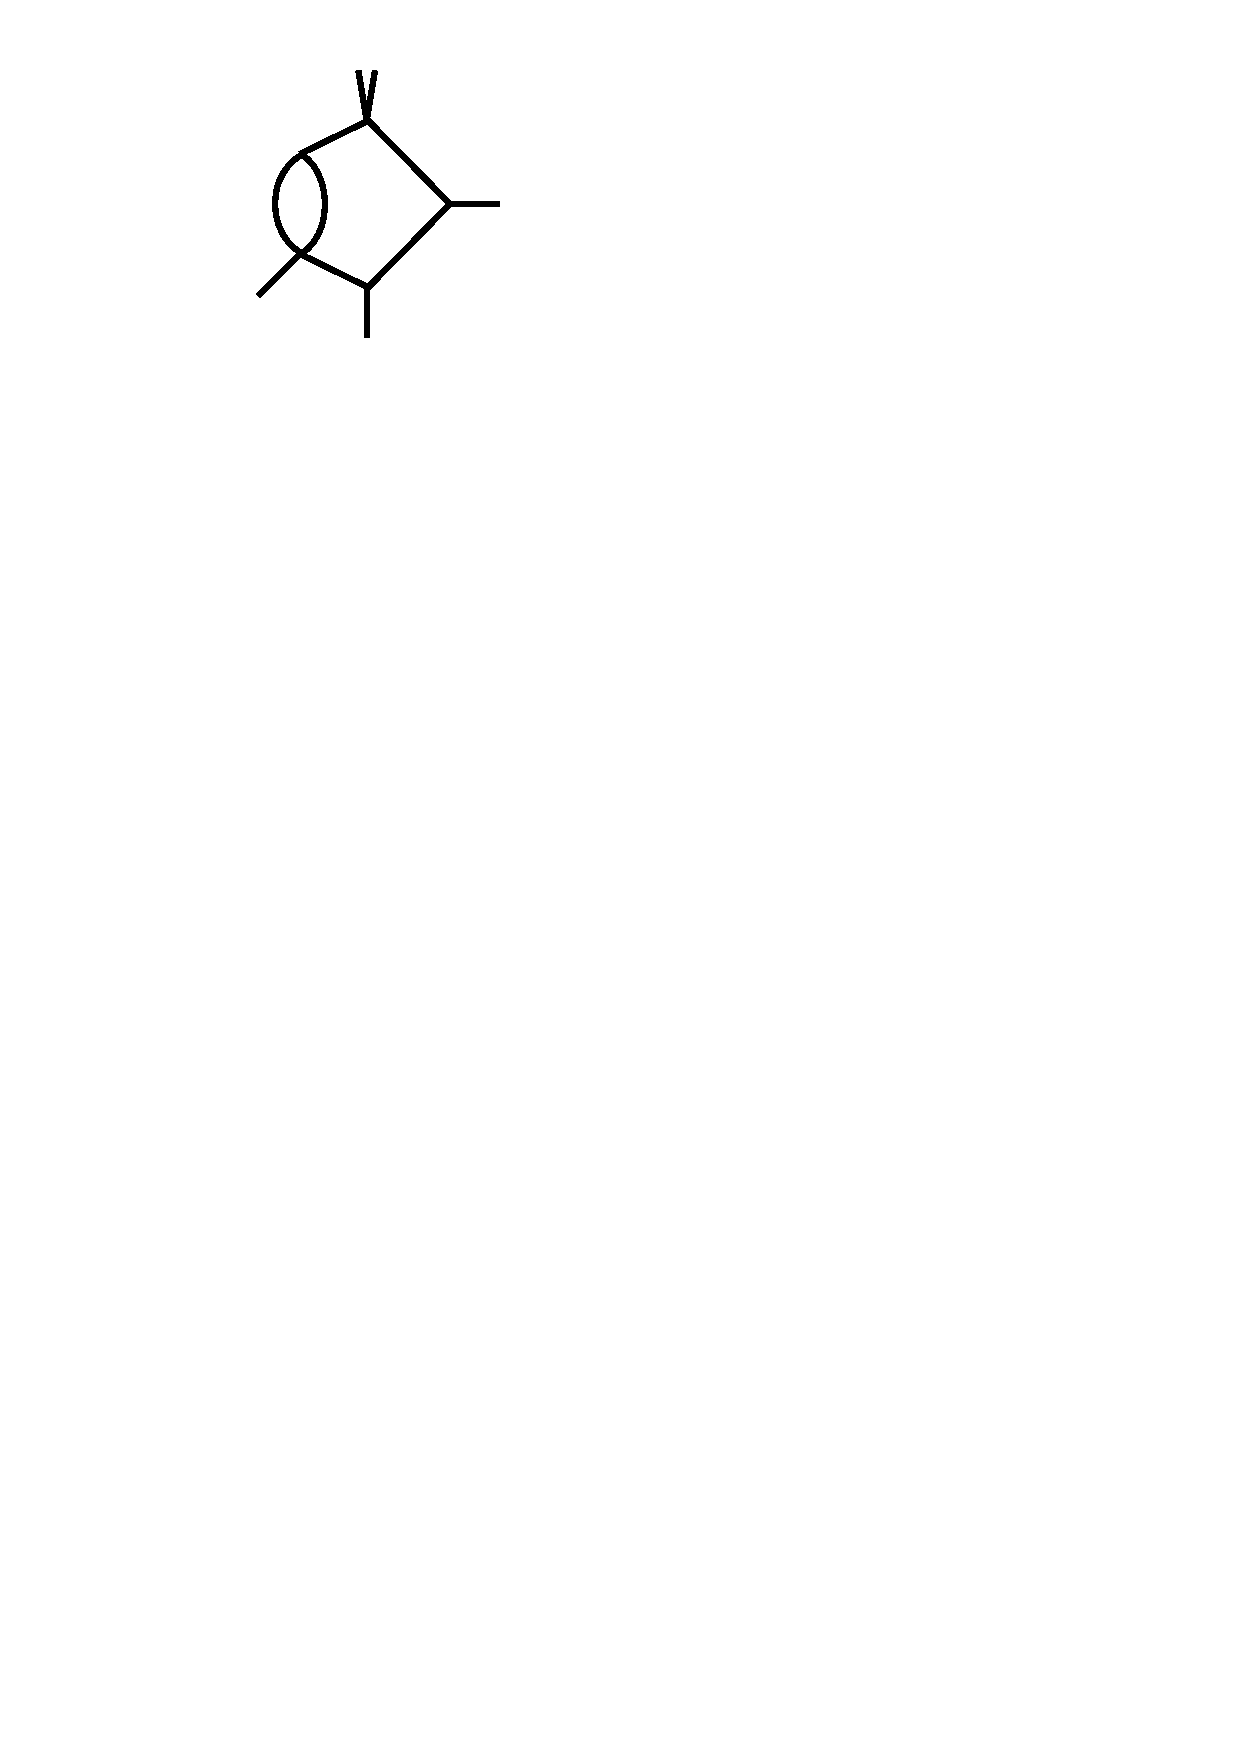
\includegraphics[scale=0.35]{figures/topologies/BubblePentagonRed5}};
    %
      \node at
      (0,-7){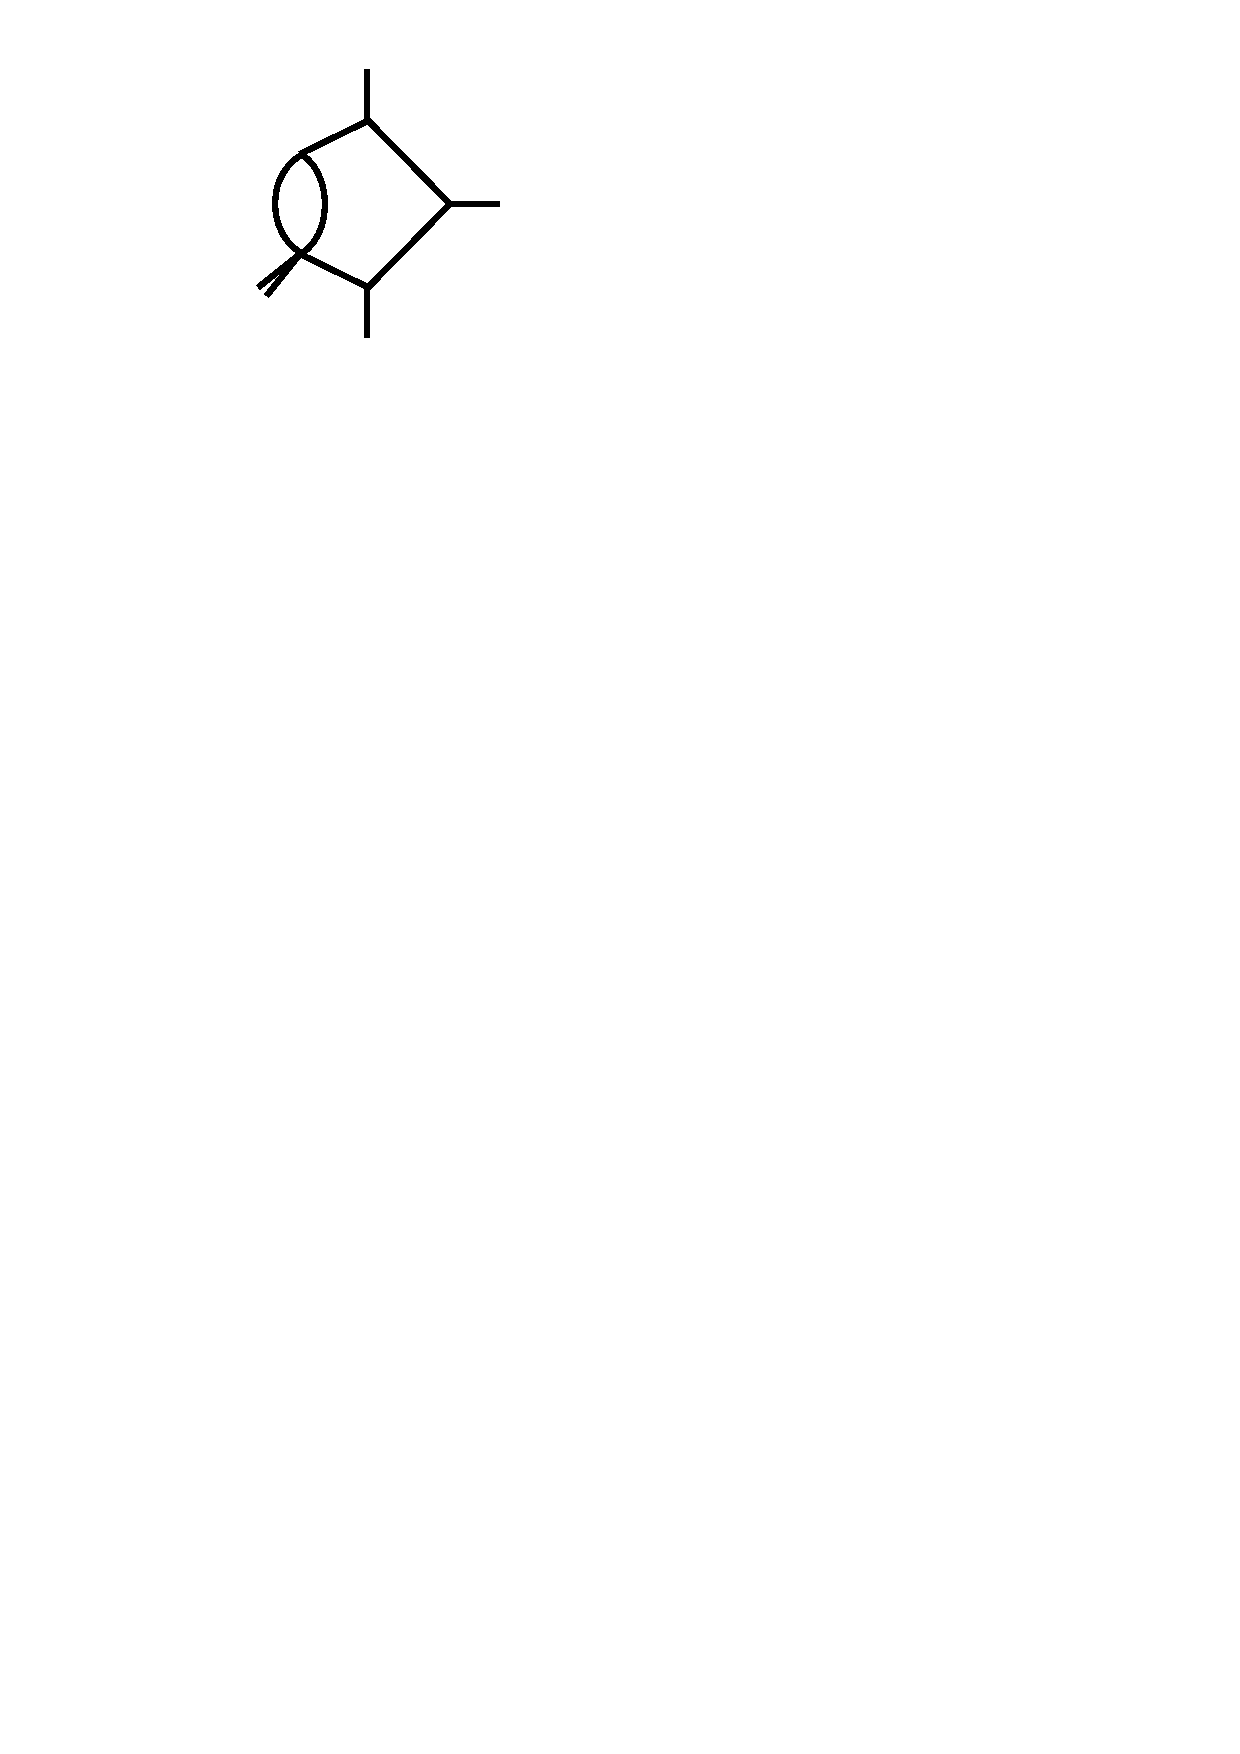
\includegraphics[scale=0.35]{figures/topologies/BubblePentagonRed6}};
      \node at
      (2,-7){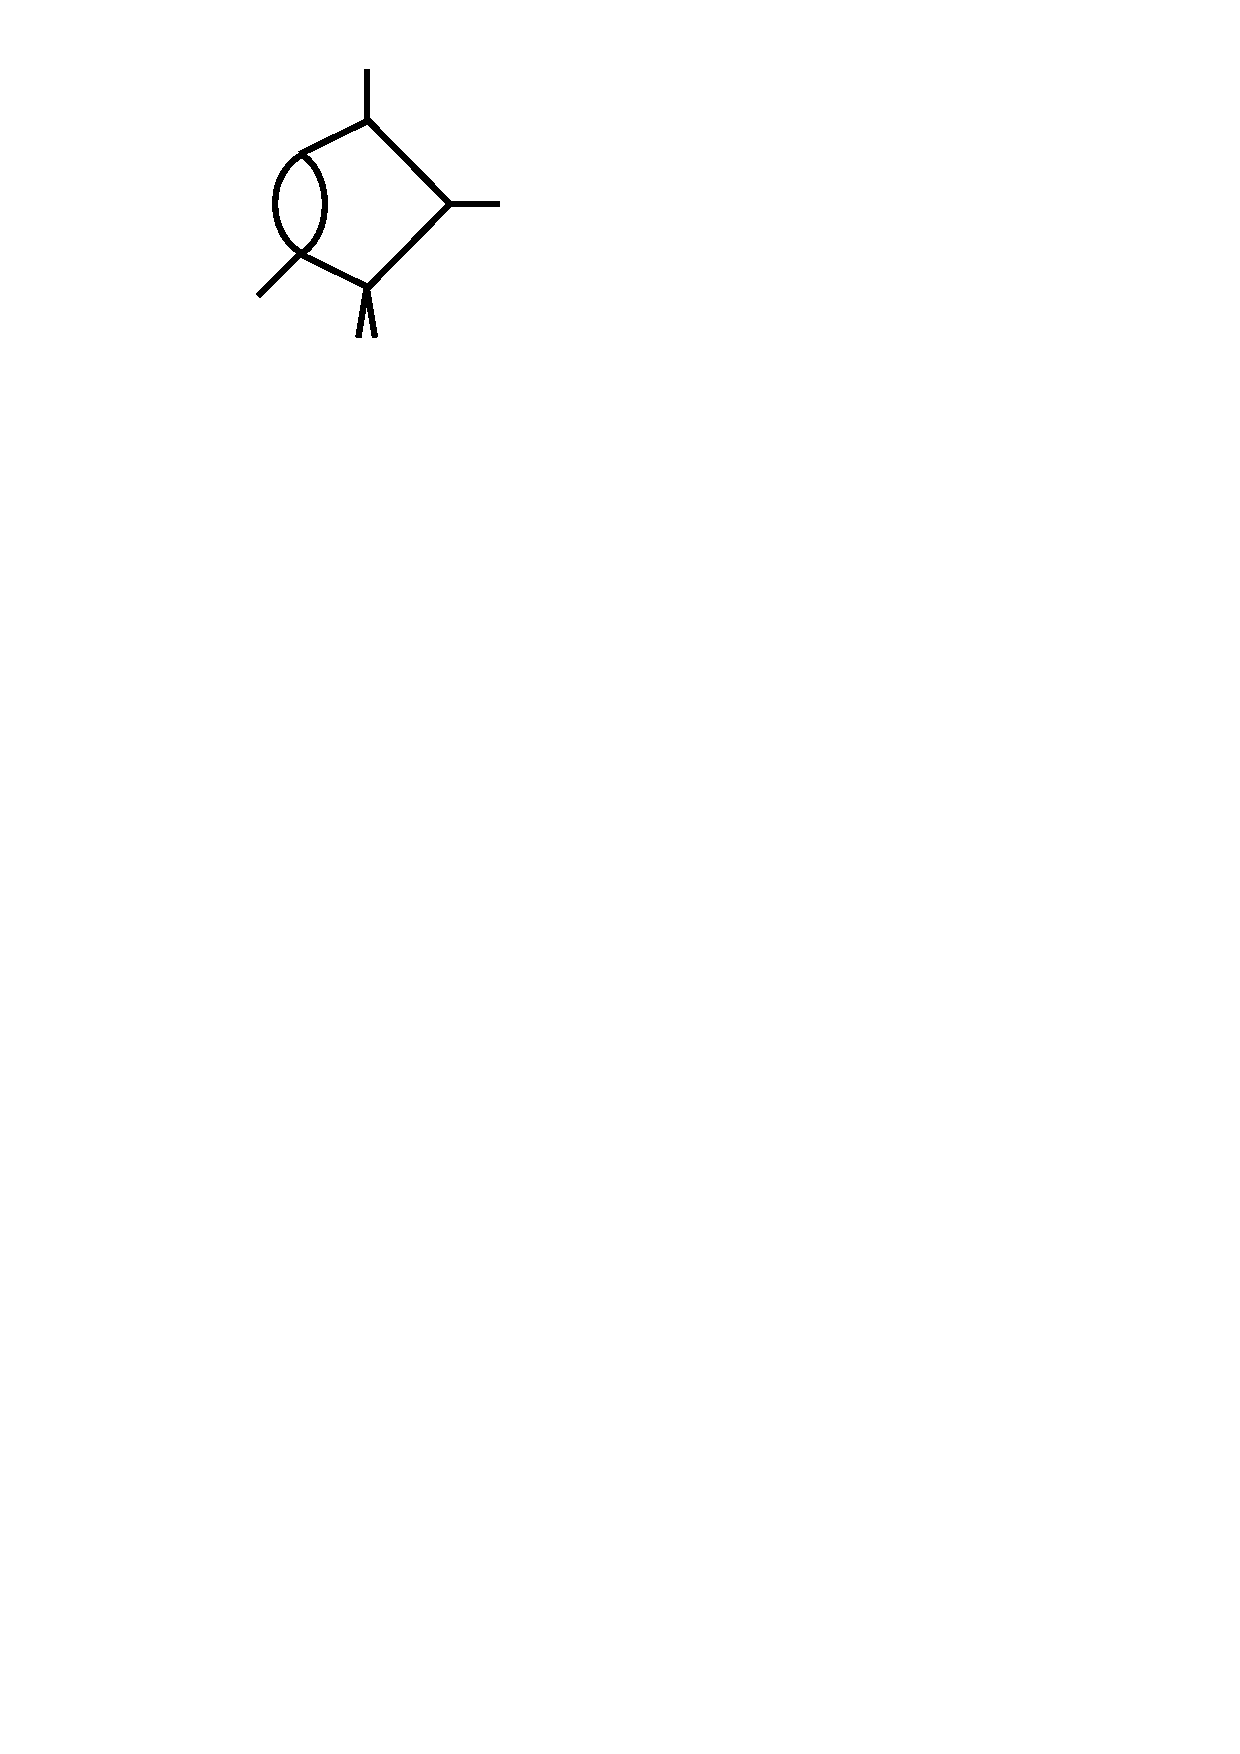
\includegraphics[scale=0.35]{figures/topologies/BubblePentagonRed7}};
      \node at
      (4,-7){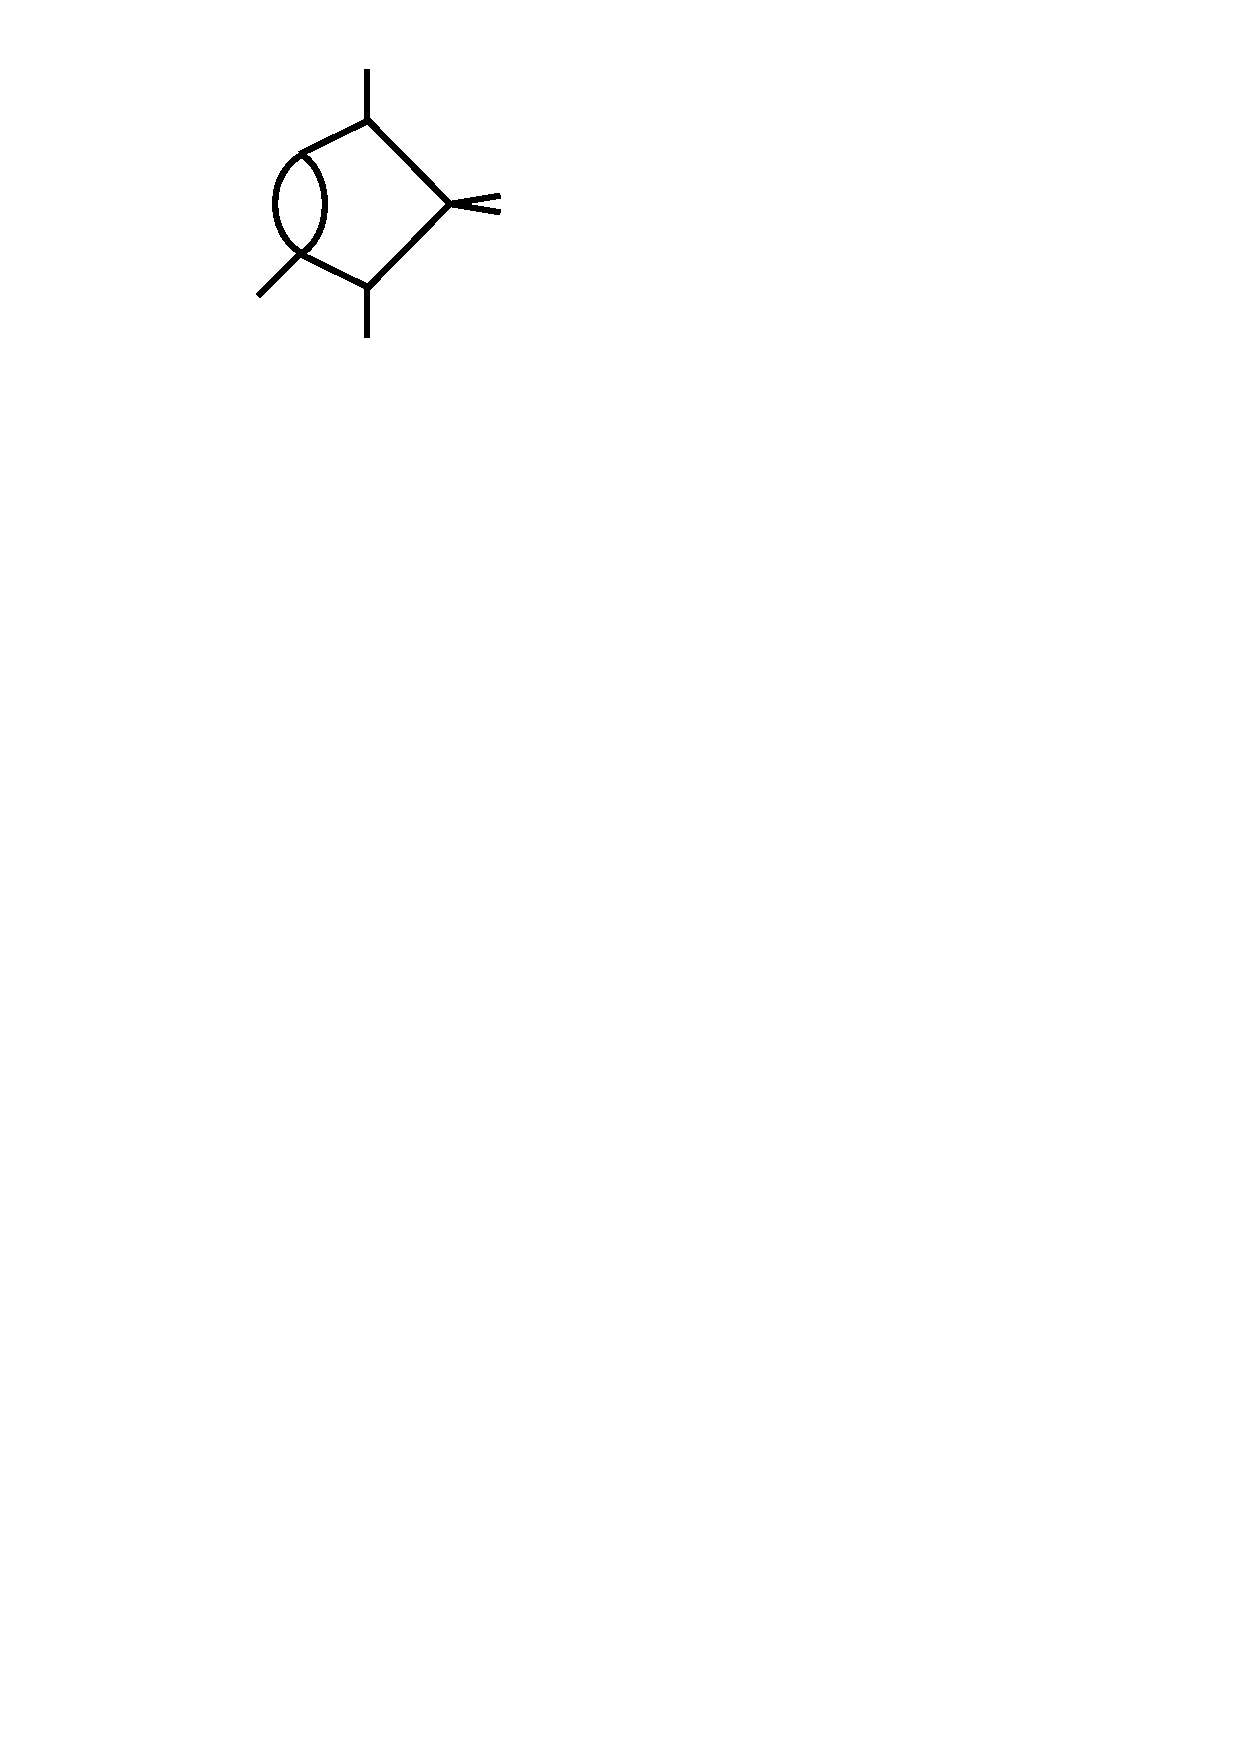
\includegraphics[scale=0.35]{figures/topologies/BubblePentagonRed8}};
      \node at
      (6,-7){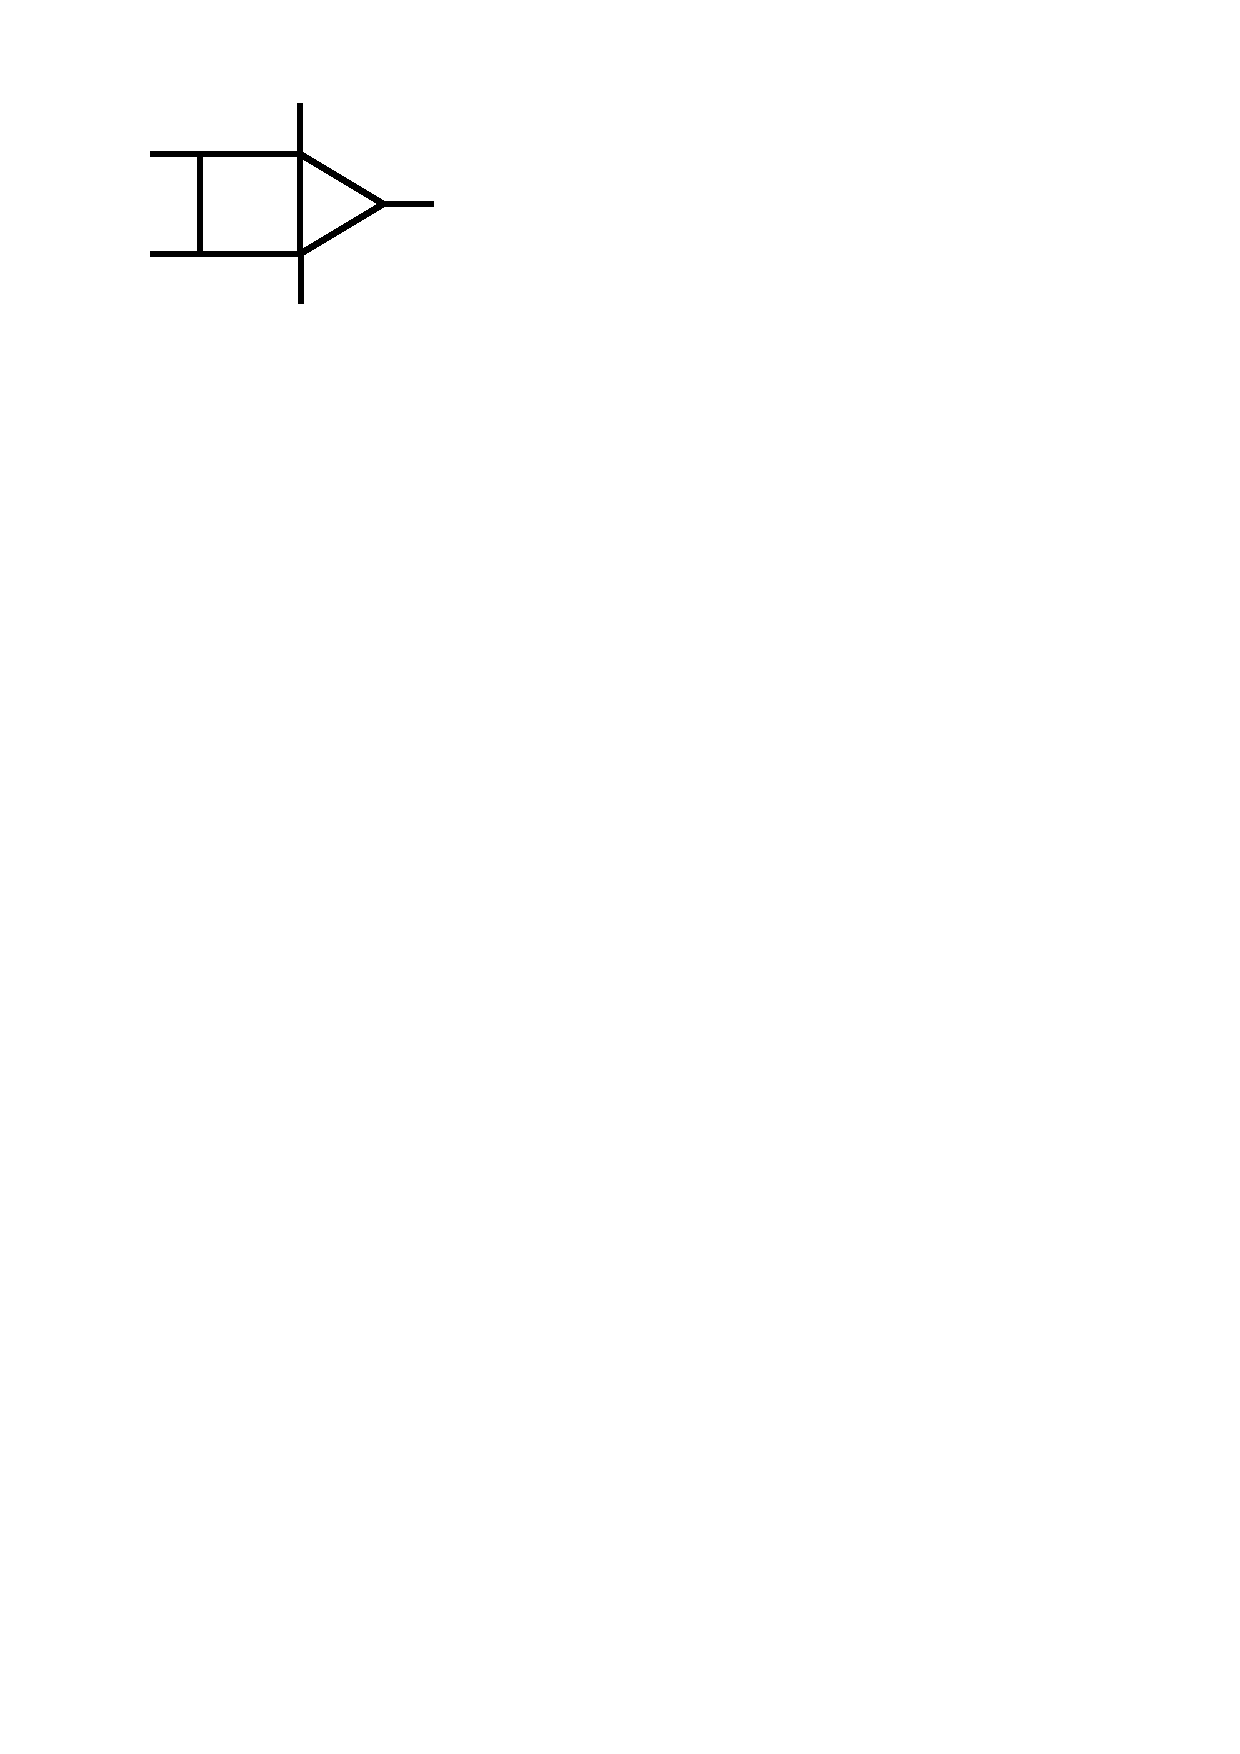
\includegraphics[scale=0.4]{figures/topologies/BoxTriangleG}};
      \node at
      (8,-6.9){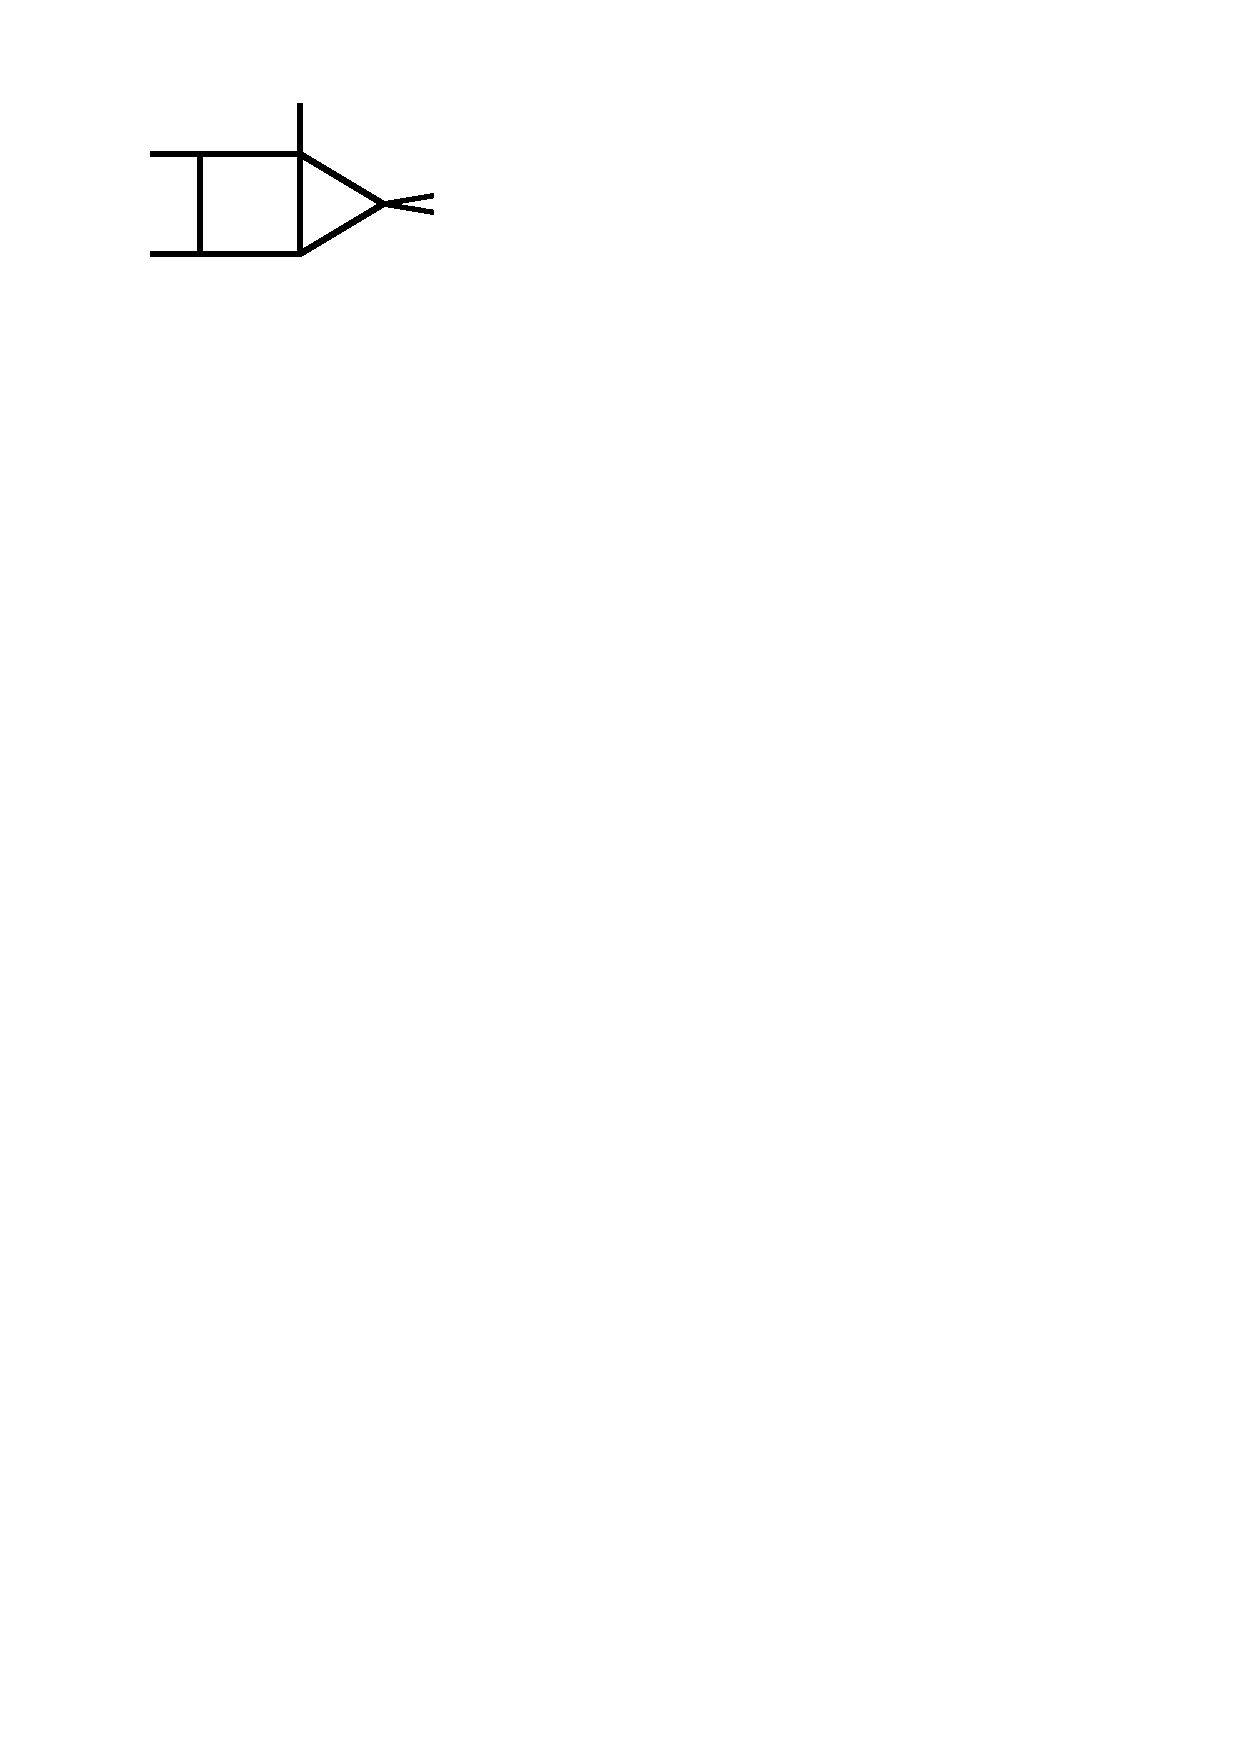
\includegraphics[scale=0.4]{figures/topologies/BoxTriangleSG}};
      \node at
      (10,-6.9){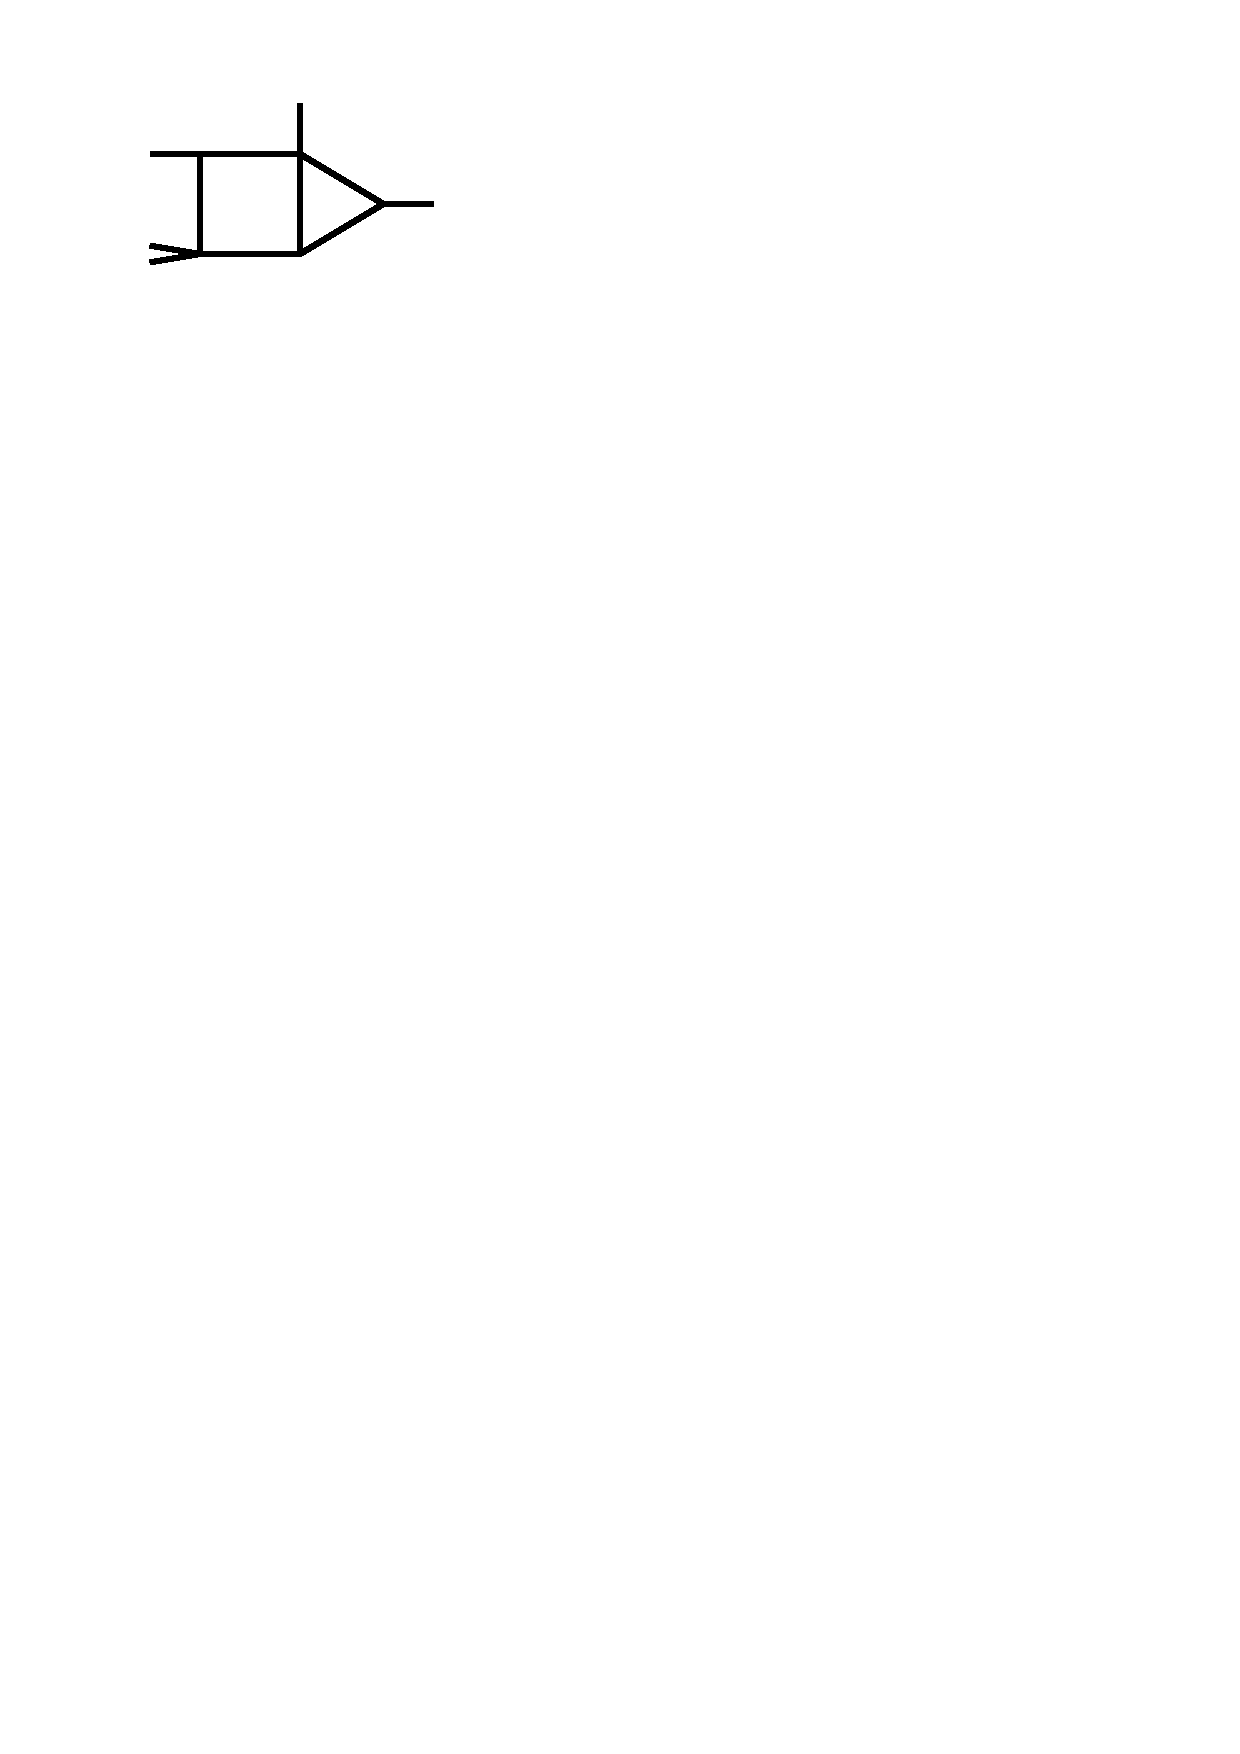
\includegraphics[scale=0.4]{figures/topologies/BoxTriangleRed1}};
    %
      \node at
      (0,-8.4){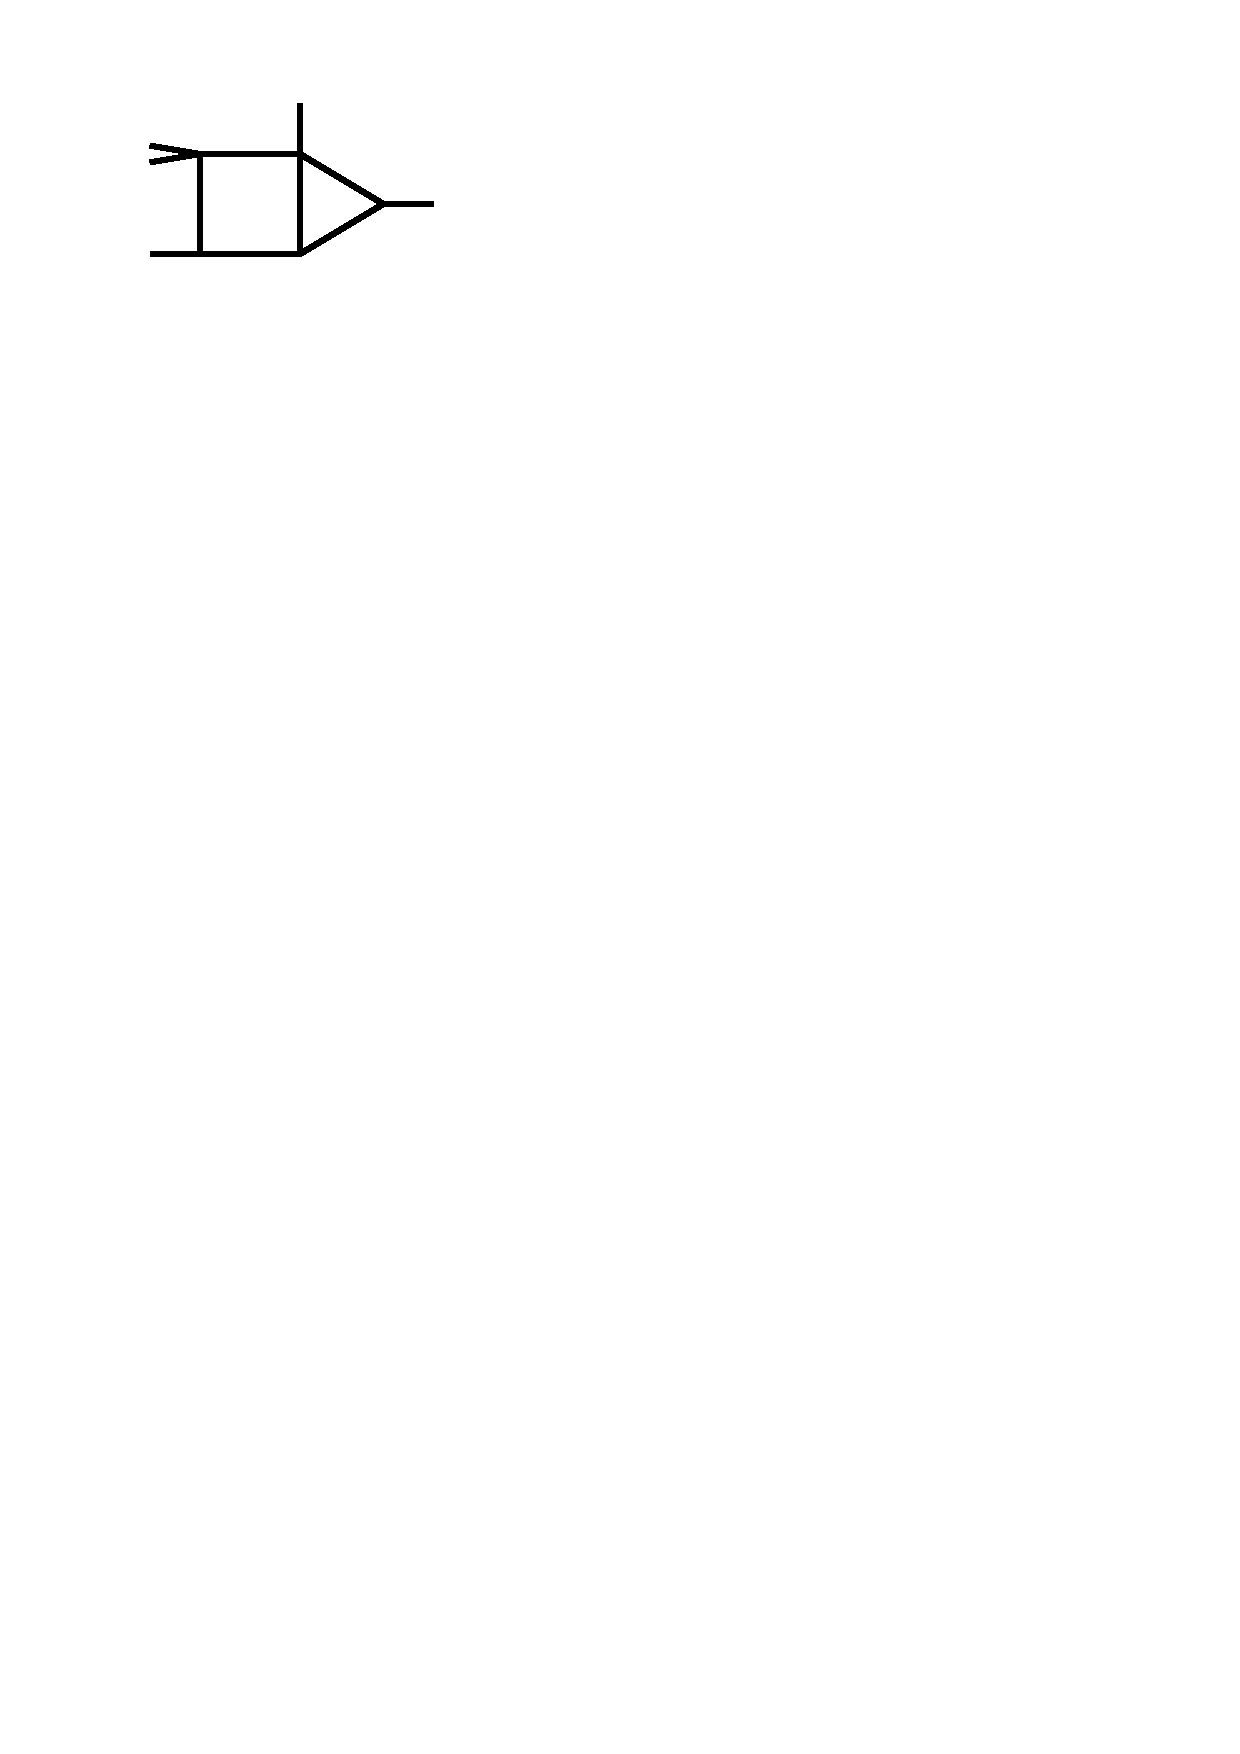
\includegraphics[scale=0.4]{figures/topologies/BoxTriangleRed2}};
      \node at
      (2,-8.4){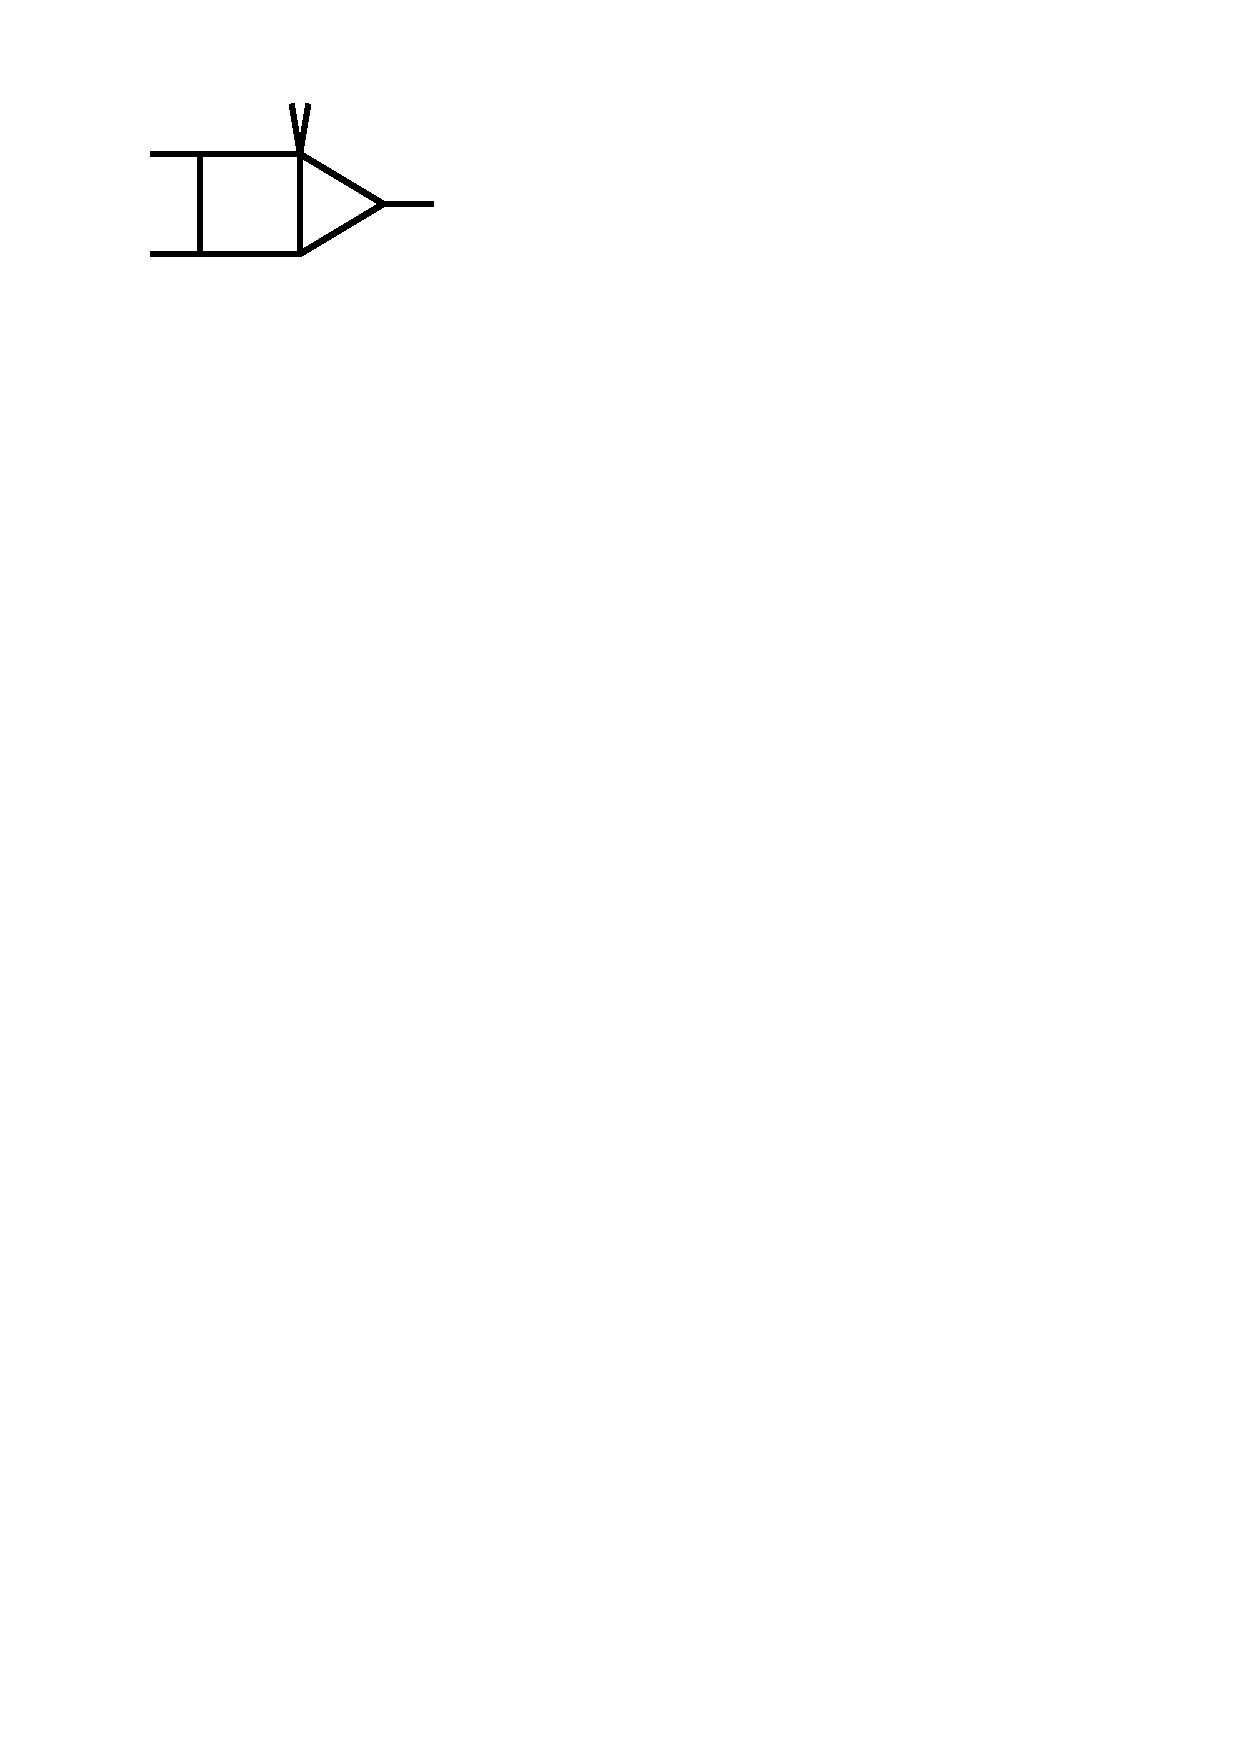
\includegraphics[scale=0.4]{figures/topologies/BoxTriangleRed3}};
      \node at
      (4,-8.5){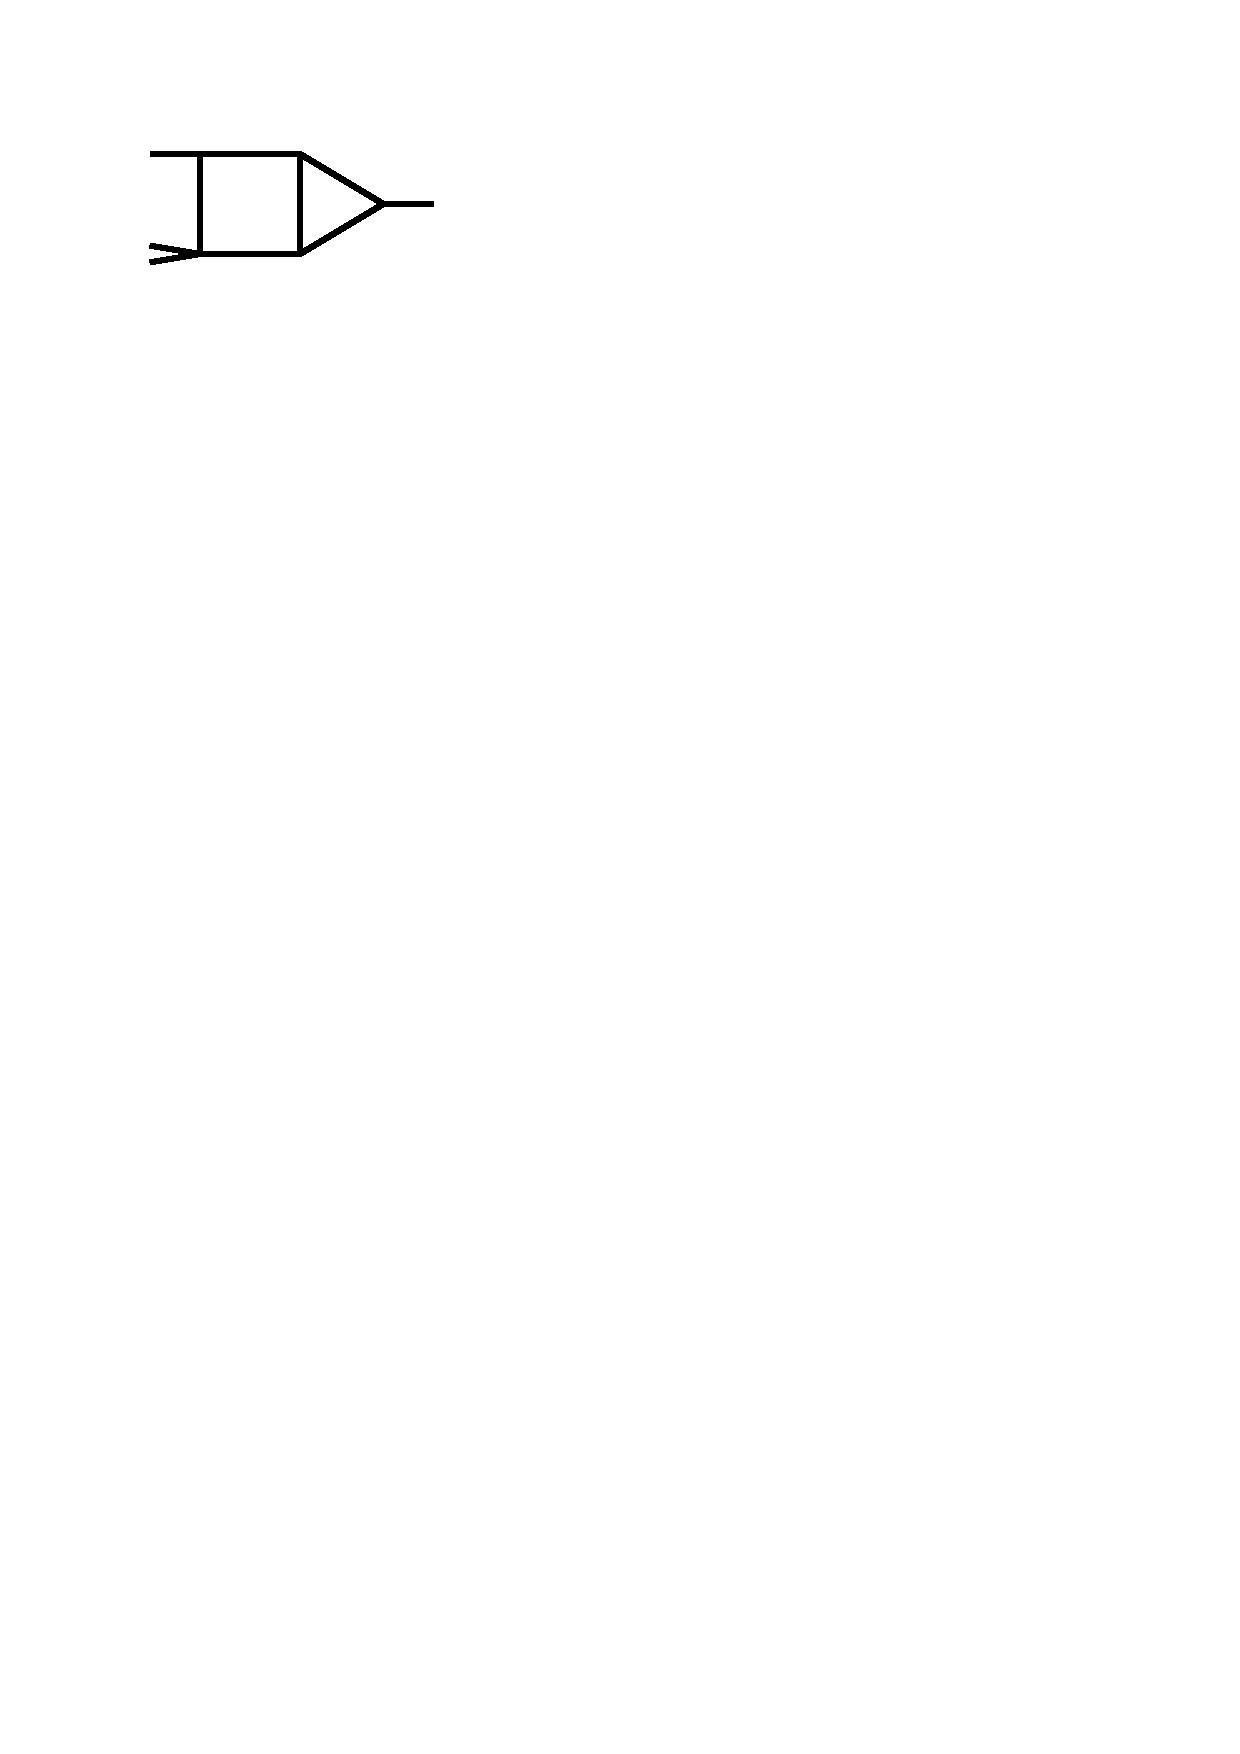
\includegraphics[scale=0.4]{figures/topologies/BoxTriangleRed4}};
      \node at
      (6,-8.5){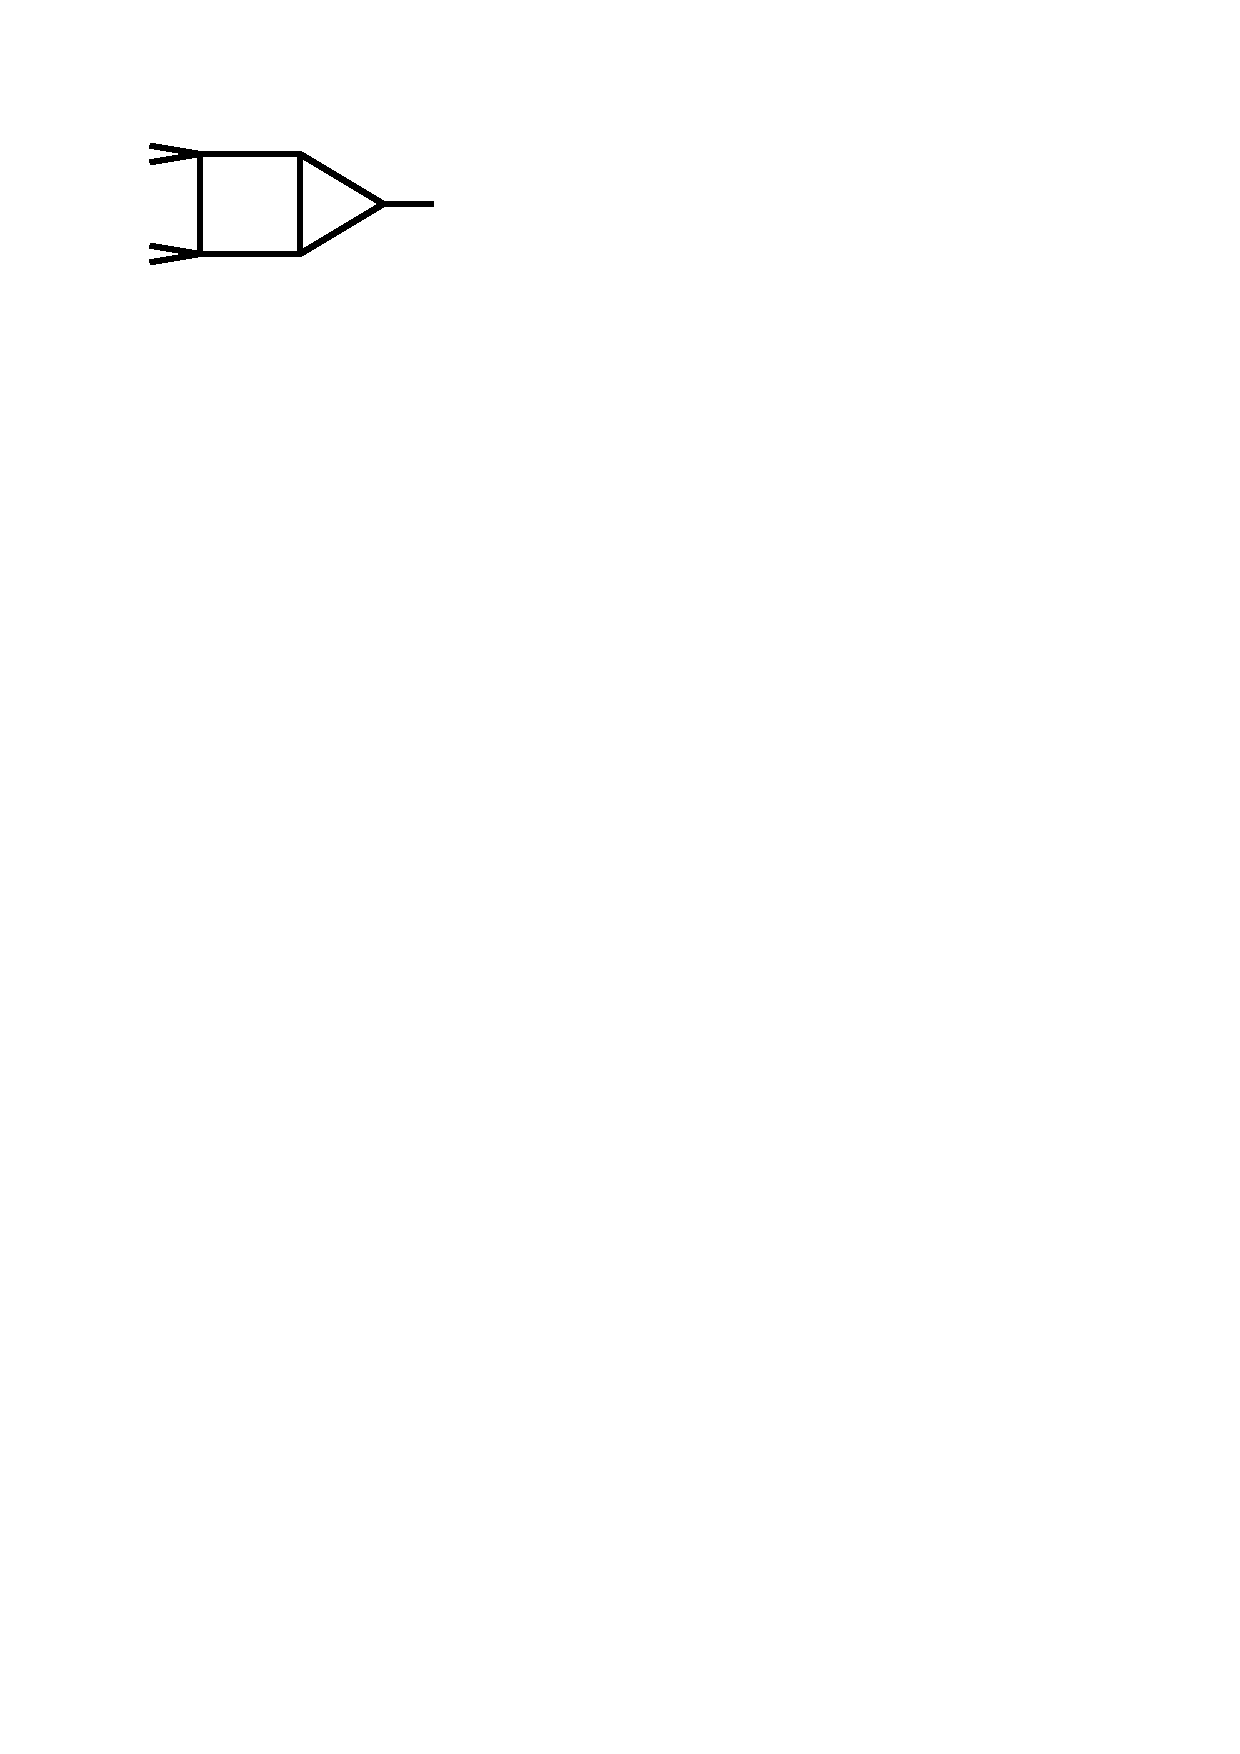
\includegraphics[scale=0.4]{figures/topologies/BoxTriangleRed5}};
      \node at
      (8,-8.5){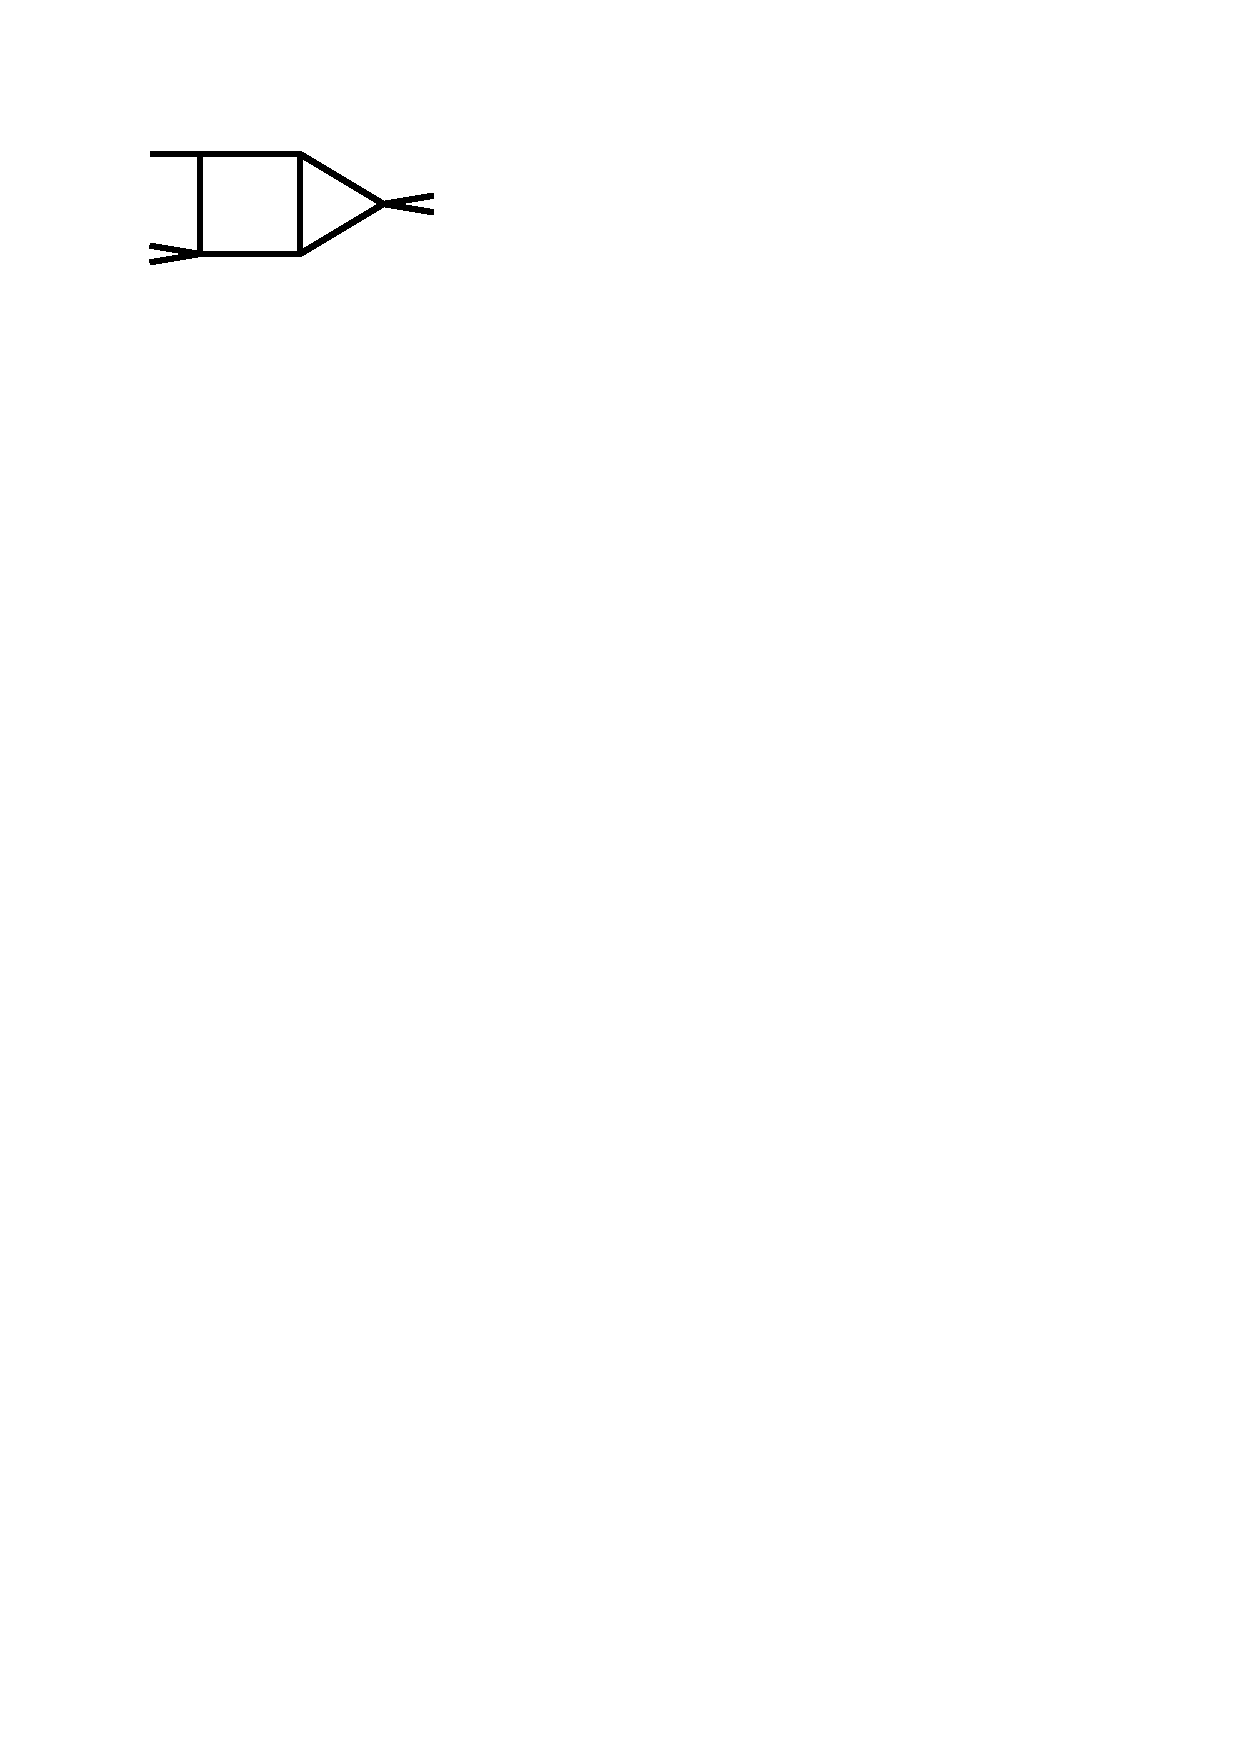
\includegraphics[scale=0.4]{figures/topologies/BoxTriangleRed6}};
      \node at
      (10,-8.5){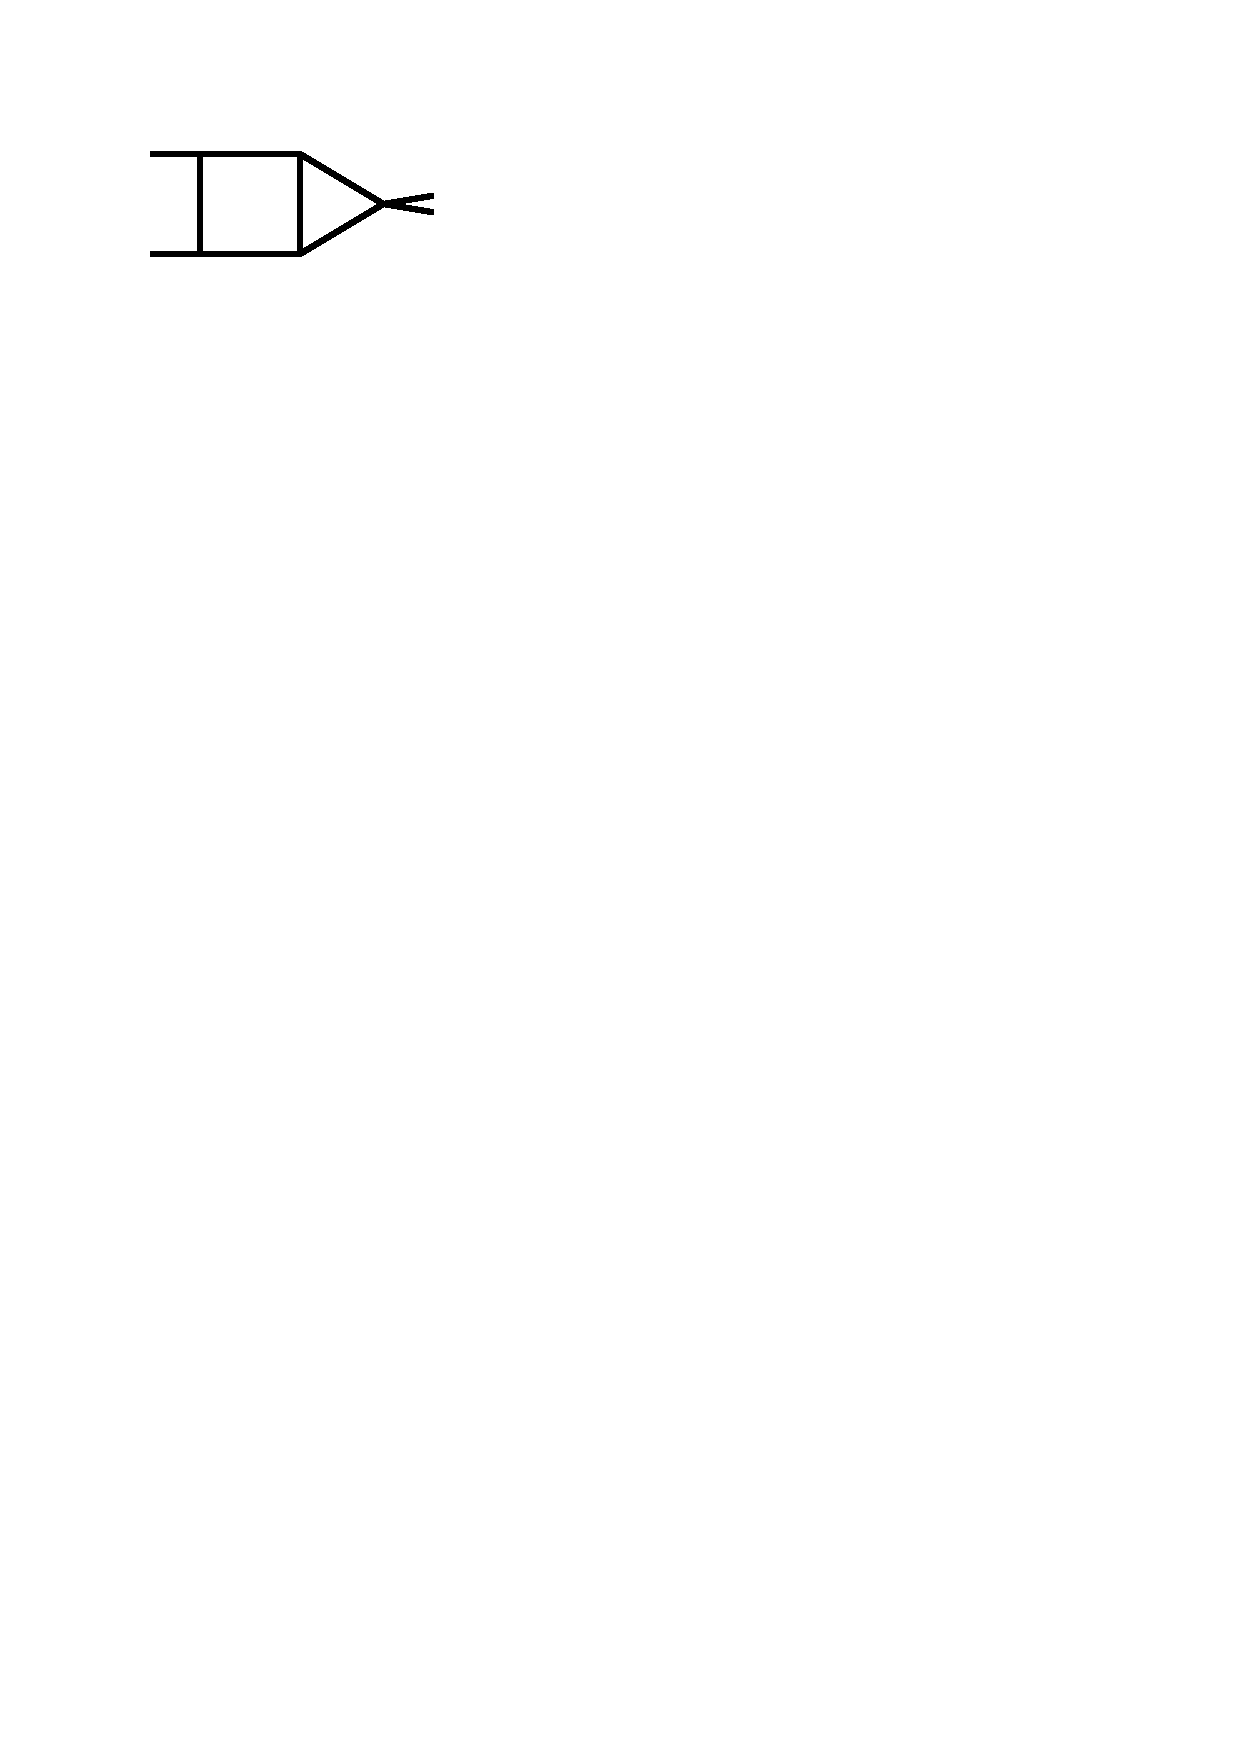
\includegraphics[scale=0.4]{figures/topologies/BoxTriangleRed7}};
    %
      \node at
      (3,-9.8){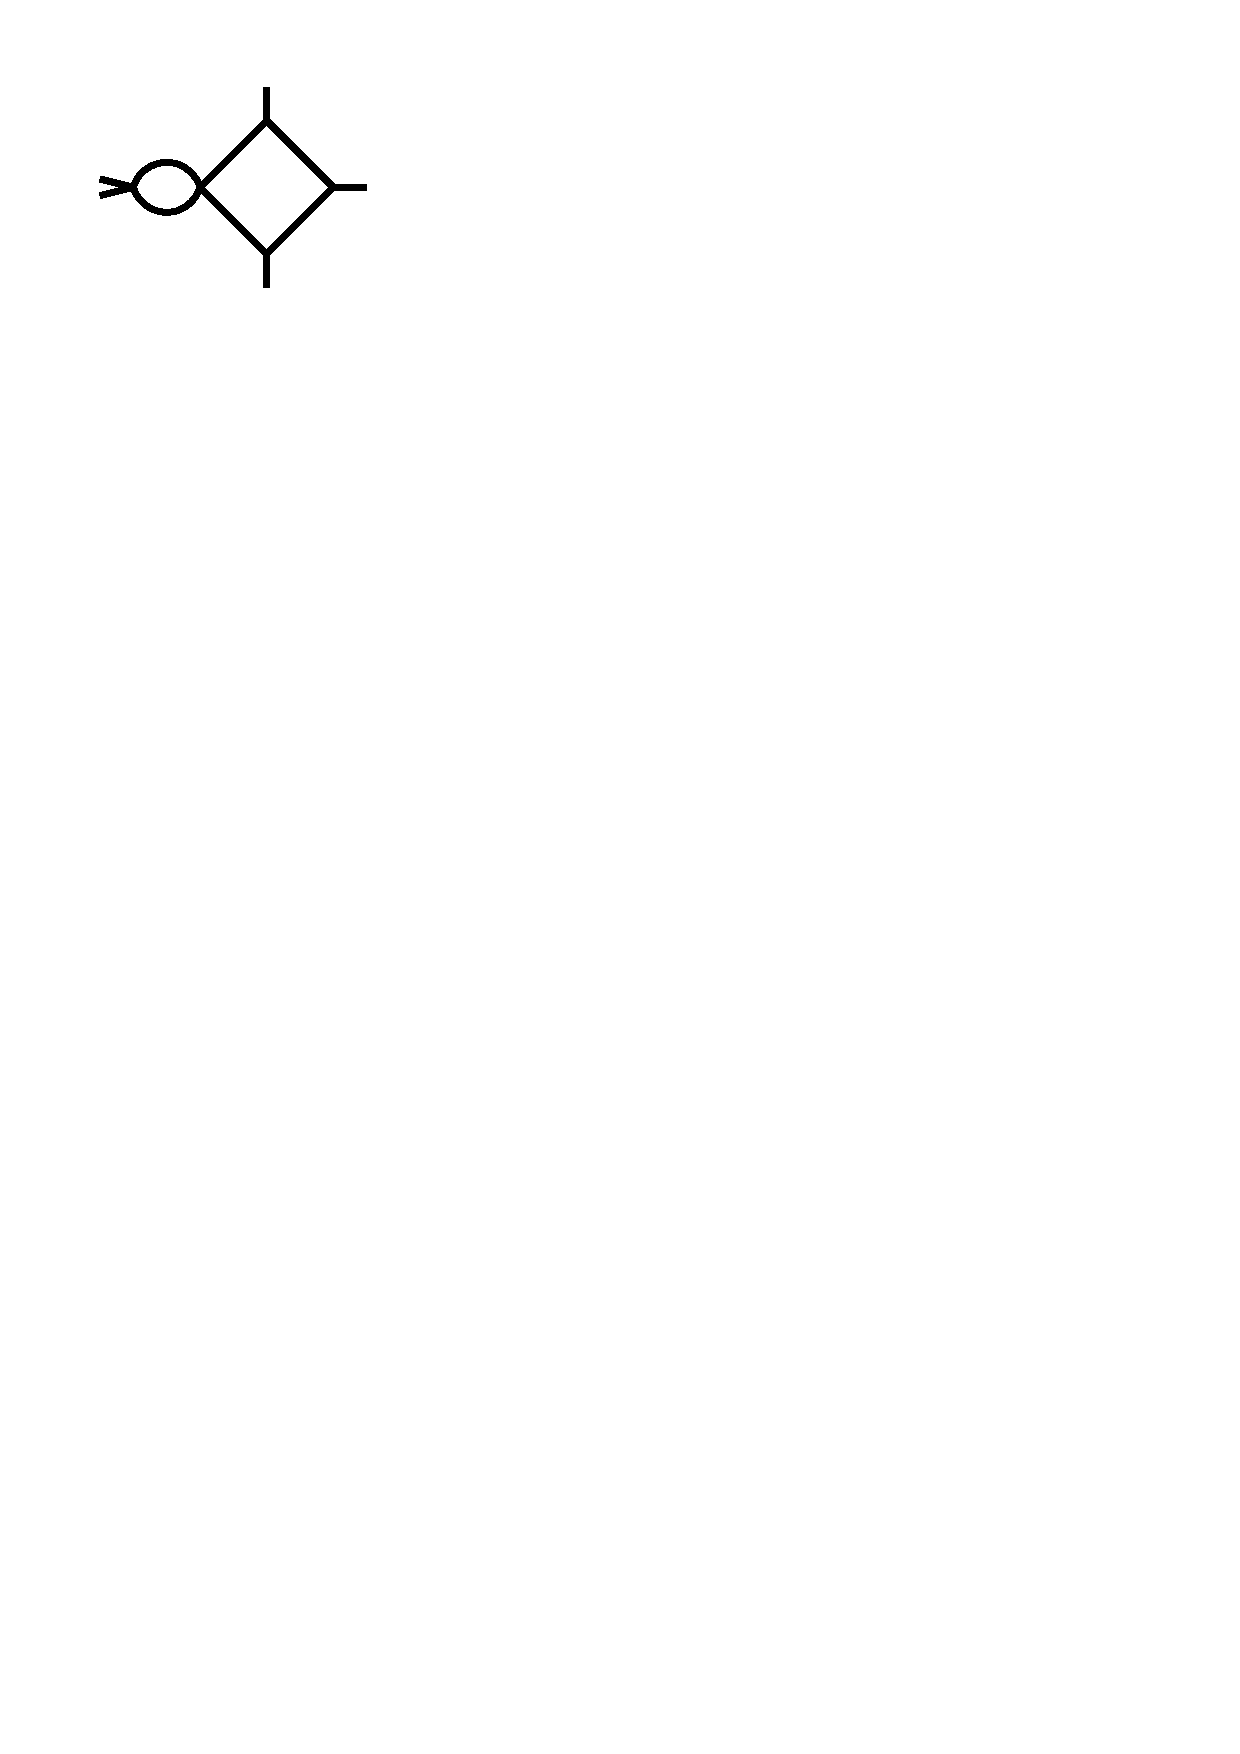
\includegraphics[scale=0.4]{figures/topologies/BoxBubble1LS}};
      \node at
      (5,-9.8){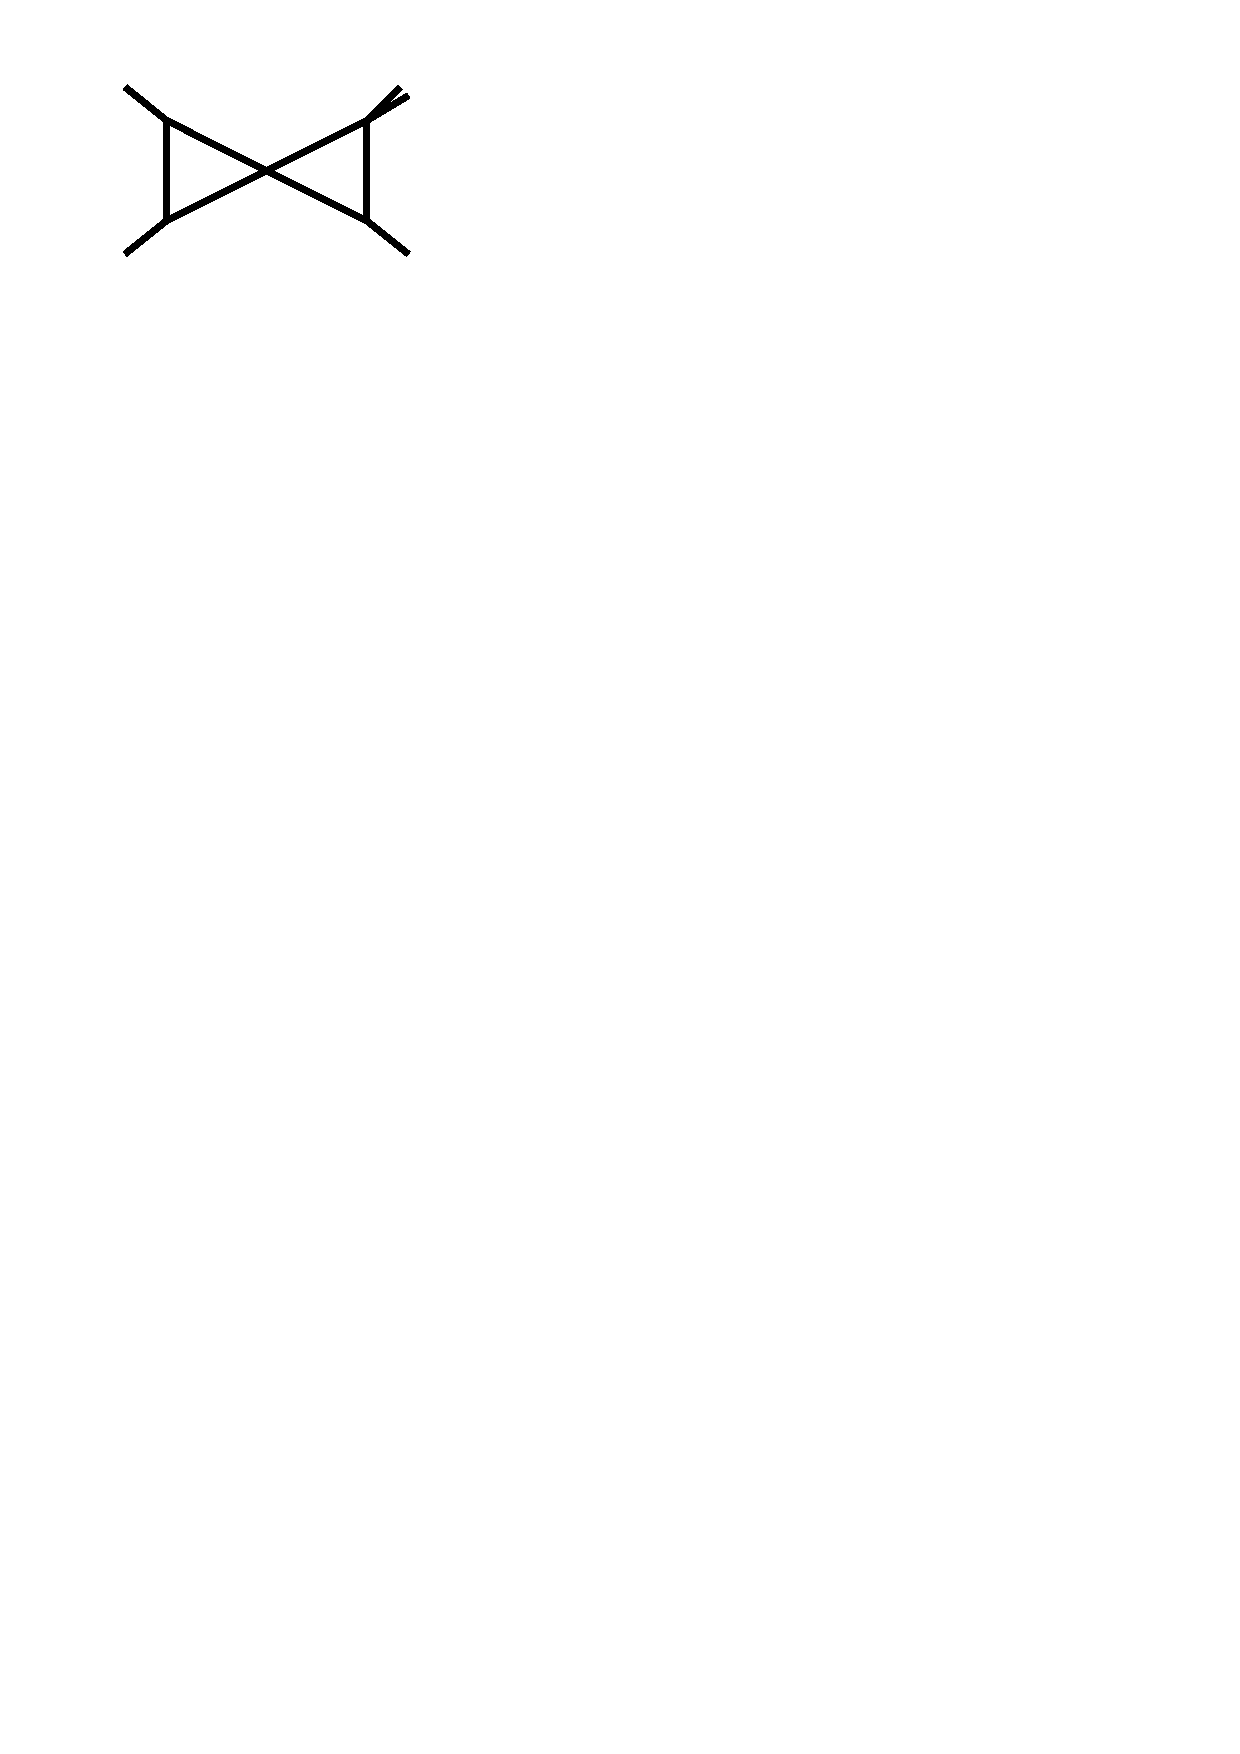
\includegraphics[scale=0.35]{figures/topologies/TriangleTriangle1LS}};
      \node at
      (7,-9.8){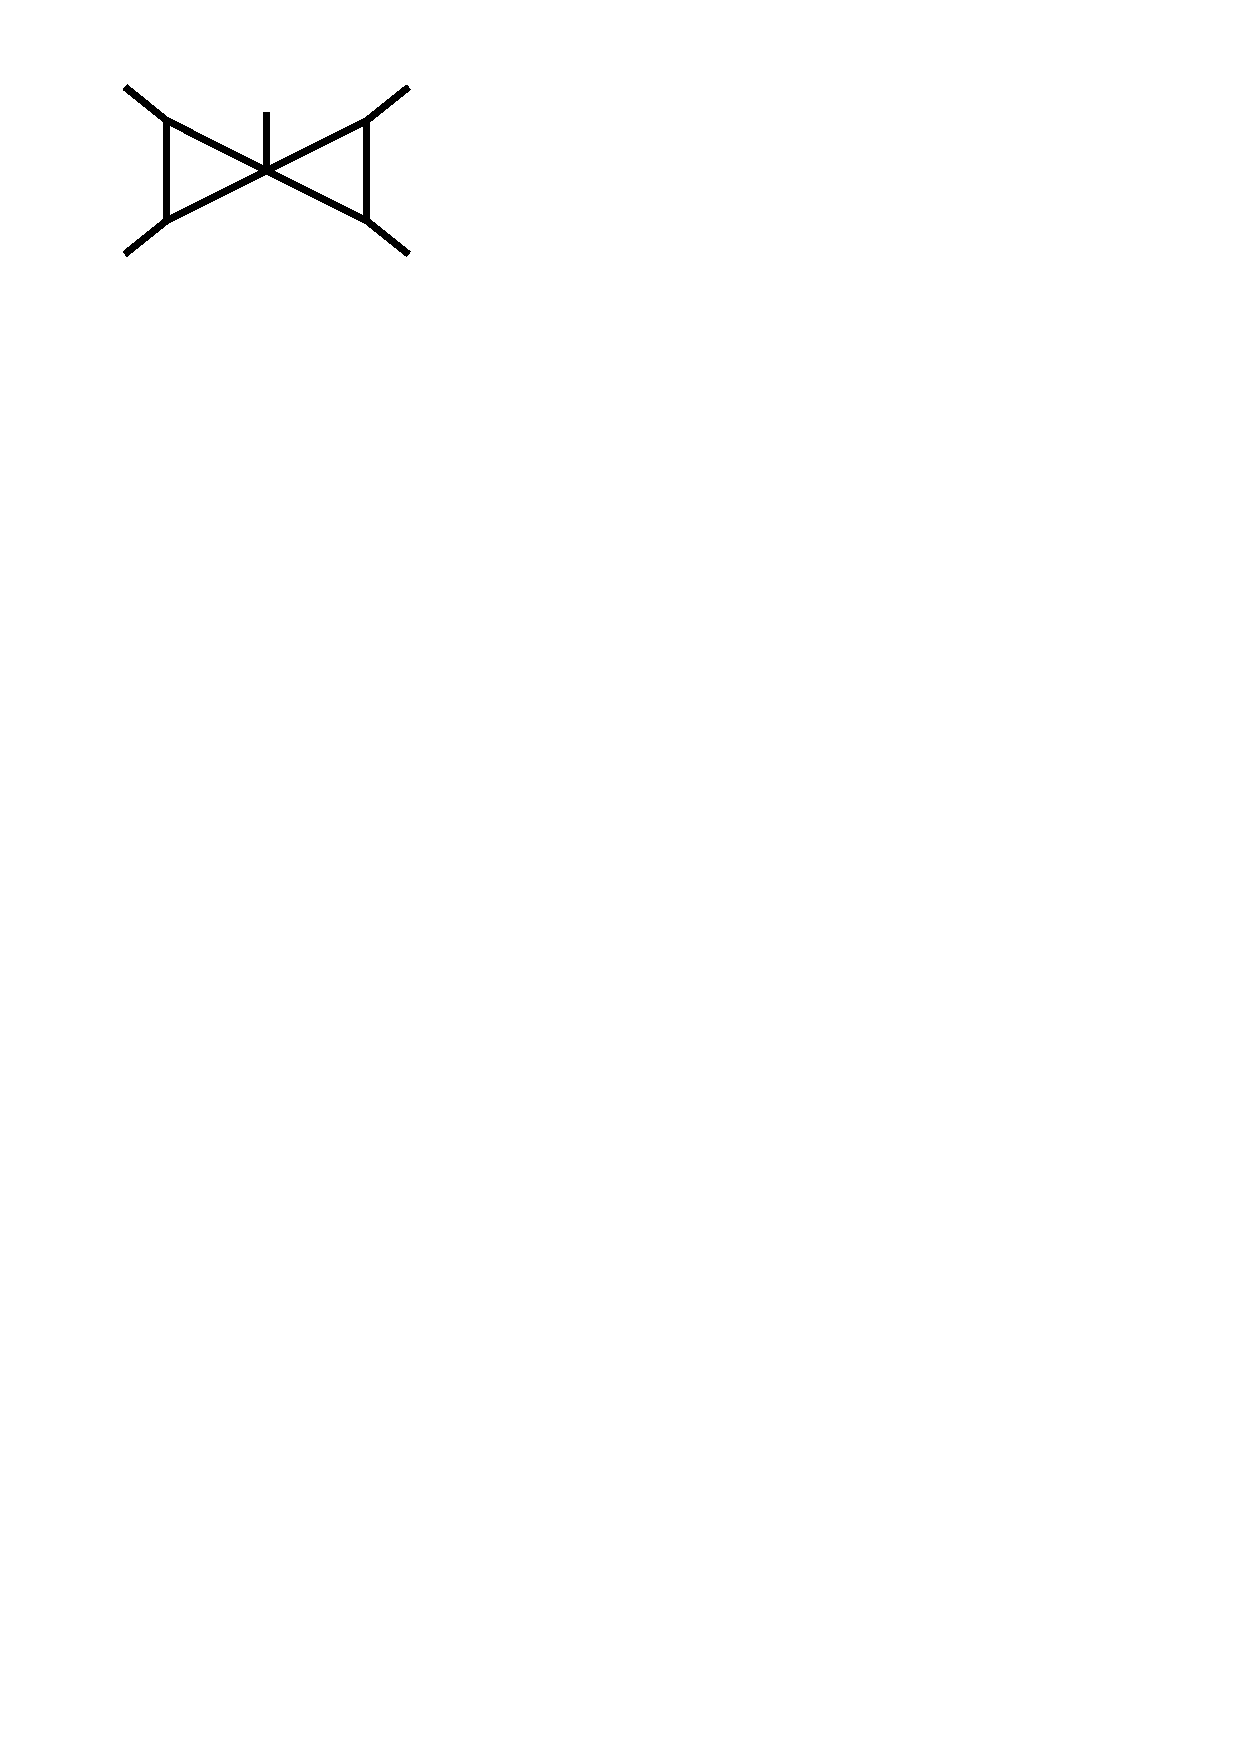
\includegraphics[scale=0.35]{figures/topologies/TriangleTriangle1LSG}};
    % Level 4
      \node at
      (0,-11.5){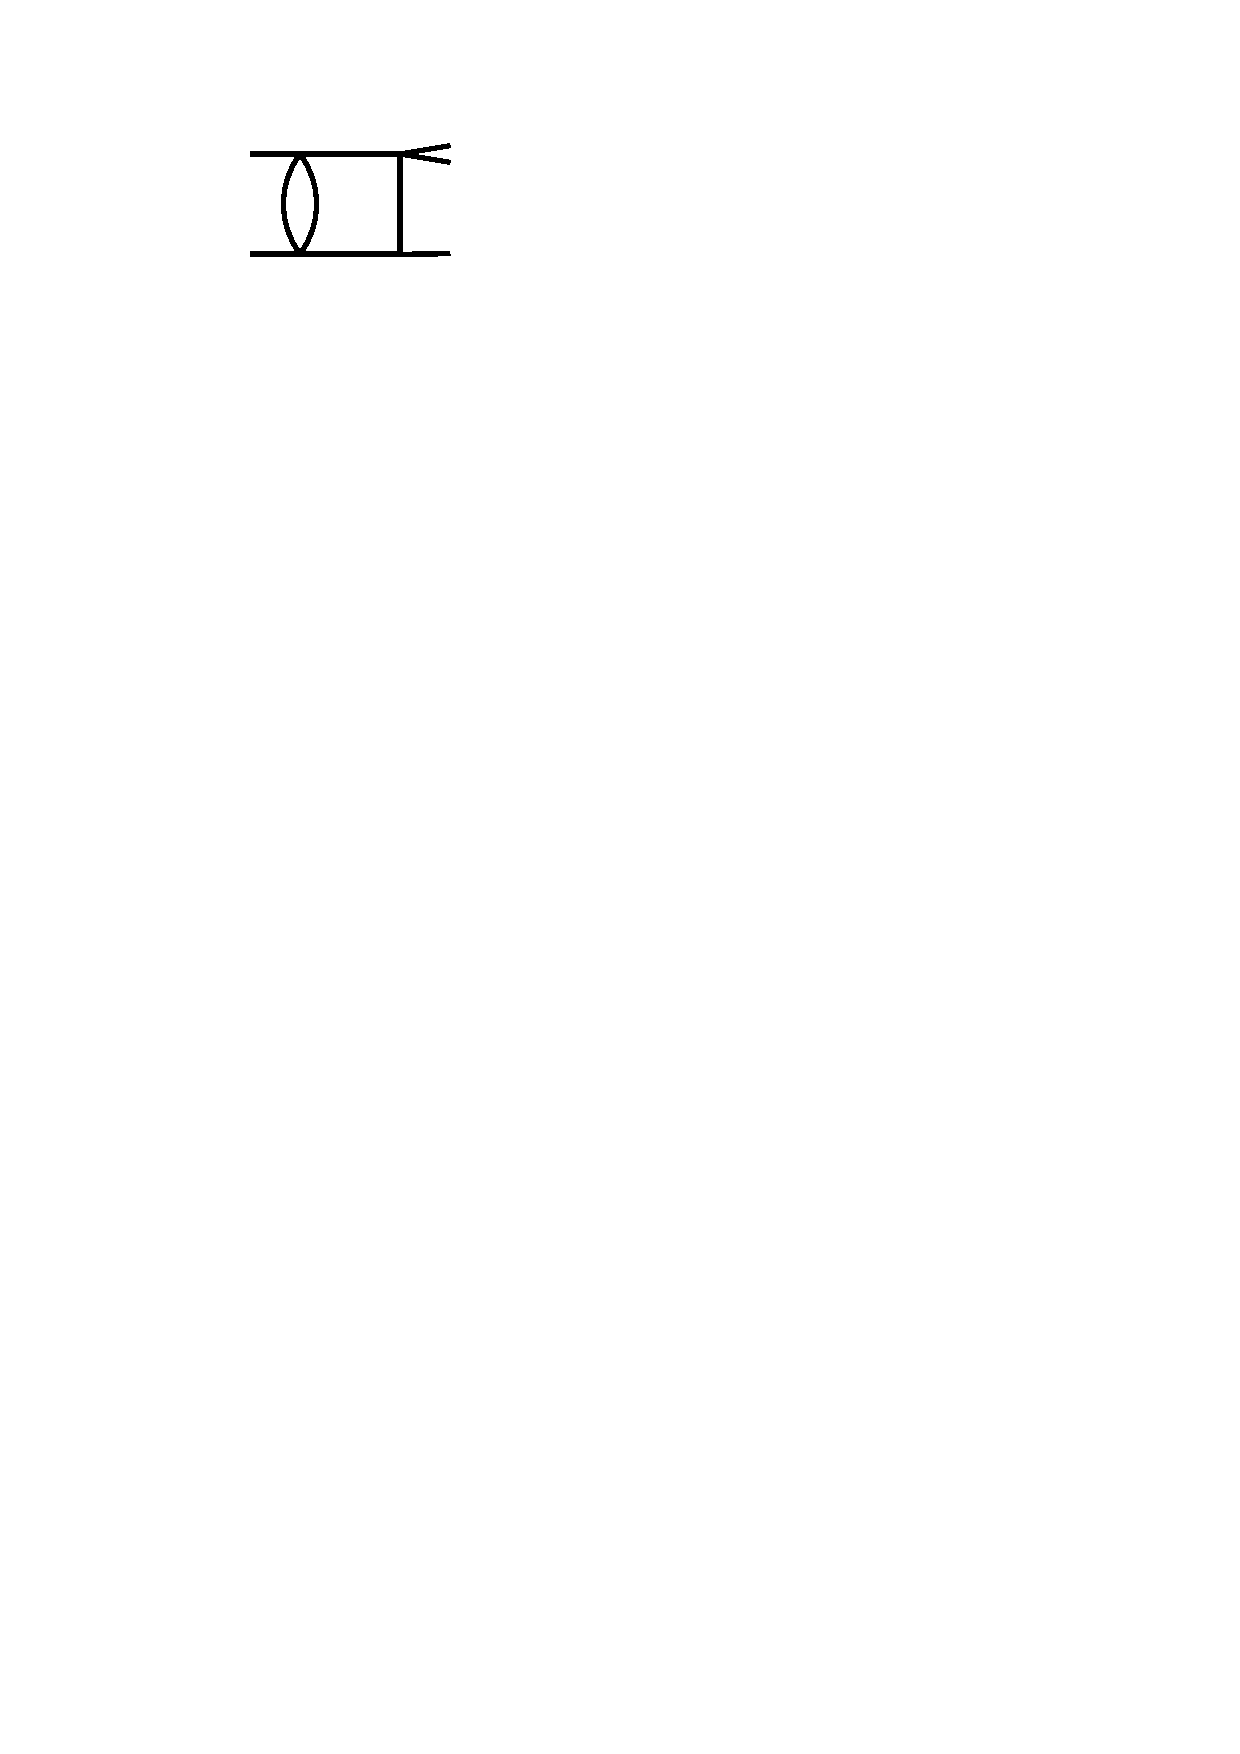
\includegraphics[scale=0.45]{figures/topologies/BoxBubbleGBox}};
      \node at
      (2,-11.5){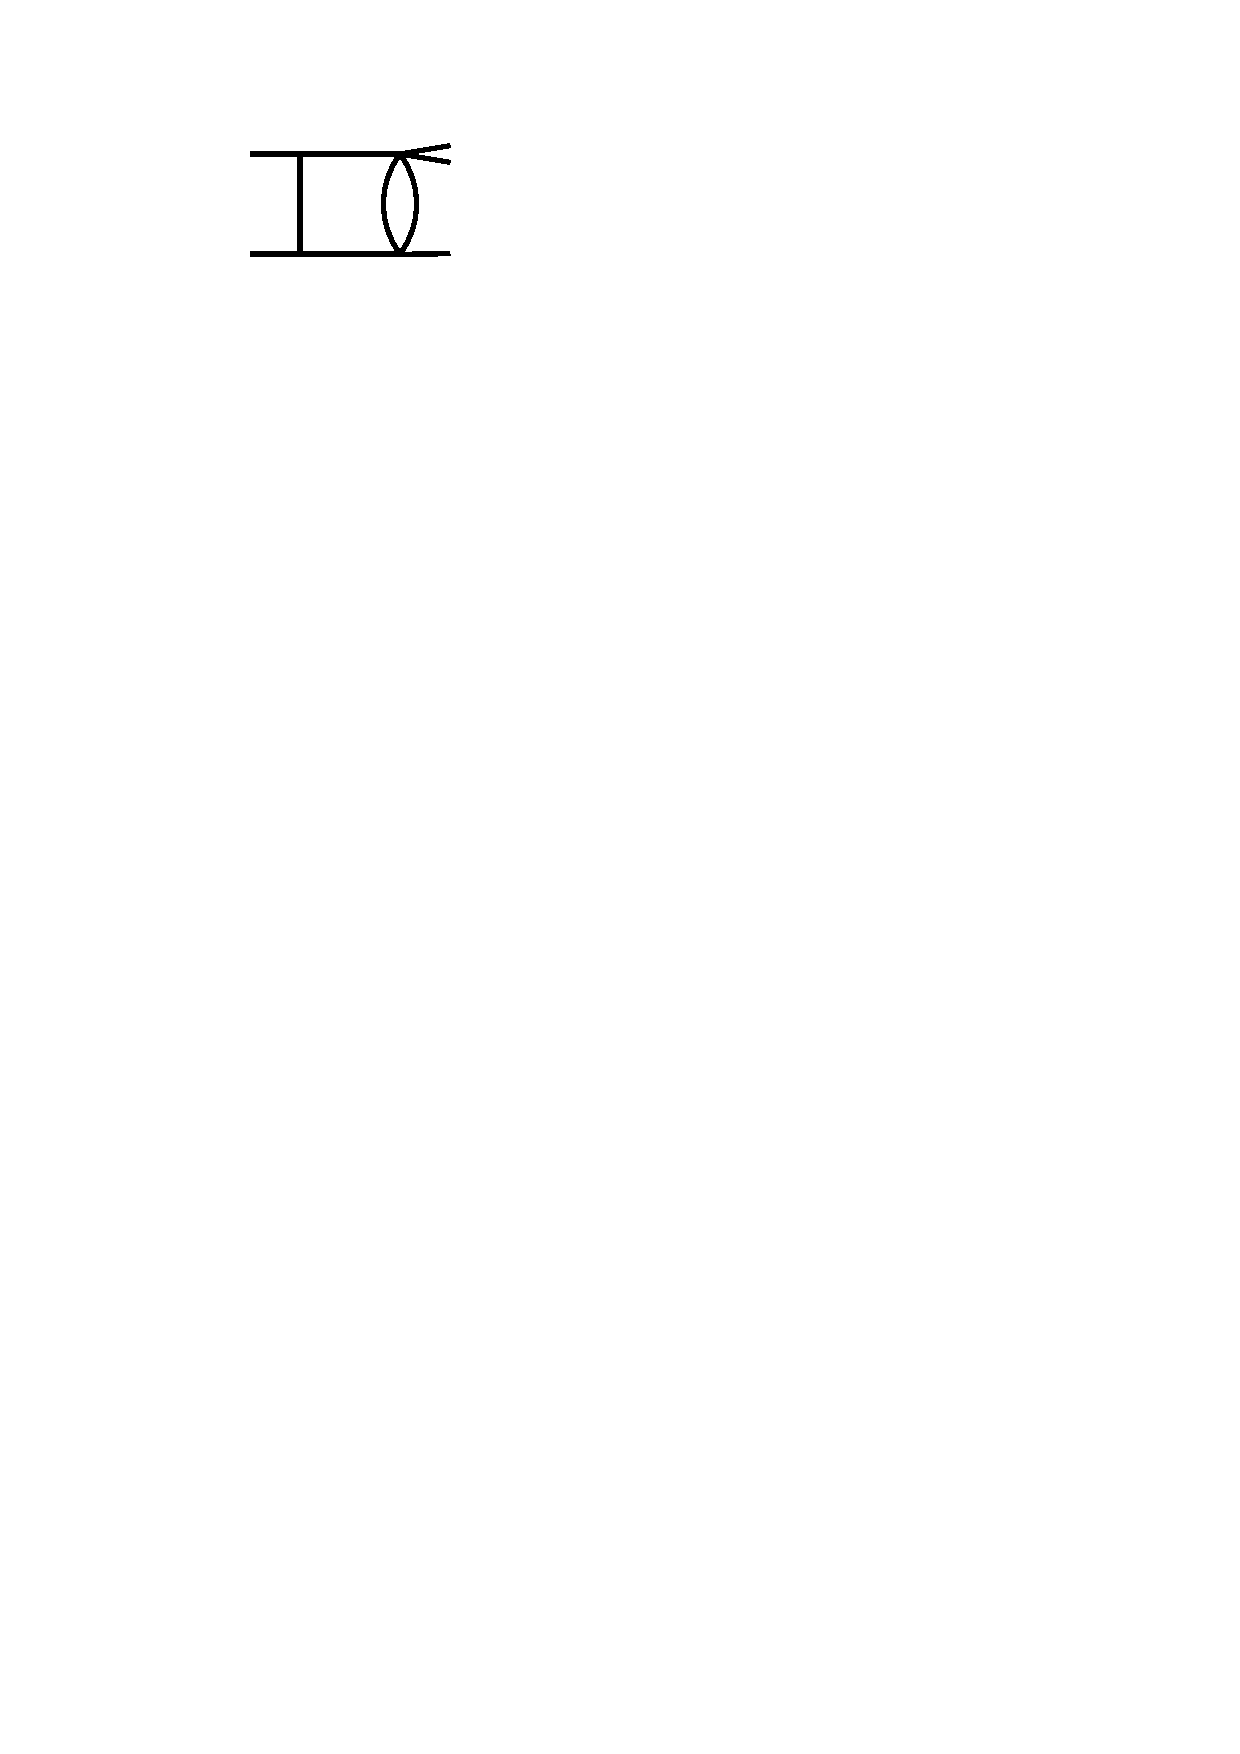
\includegraphics[scale=0.45]{figures/topologies/BoxBubbleGBub}};
      \node at
      (4,-11.5){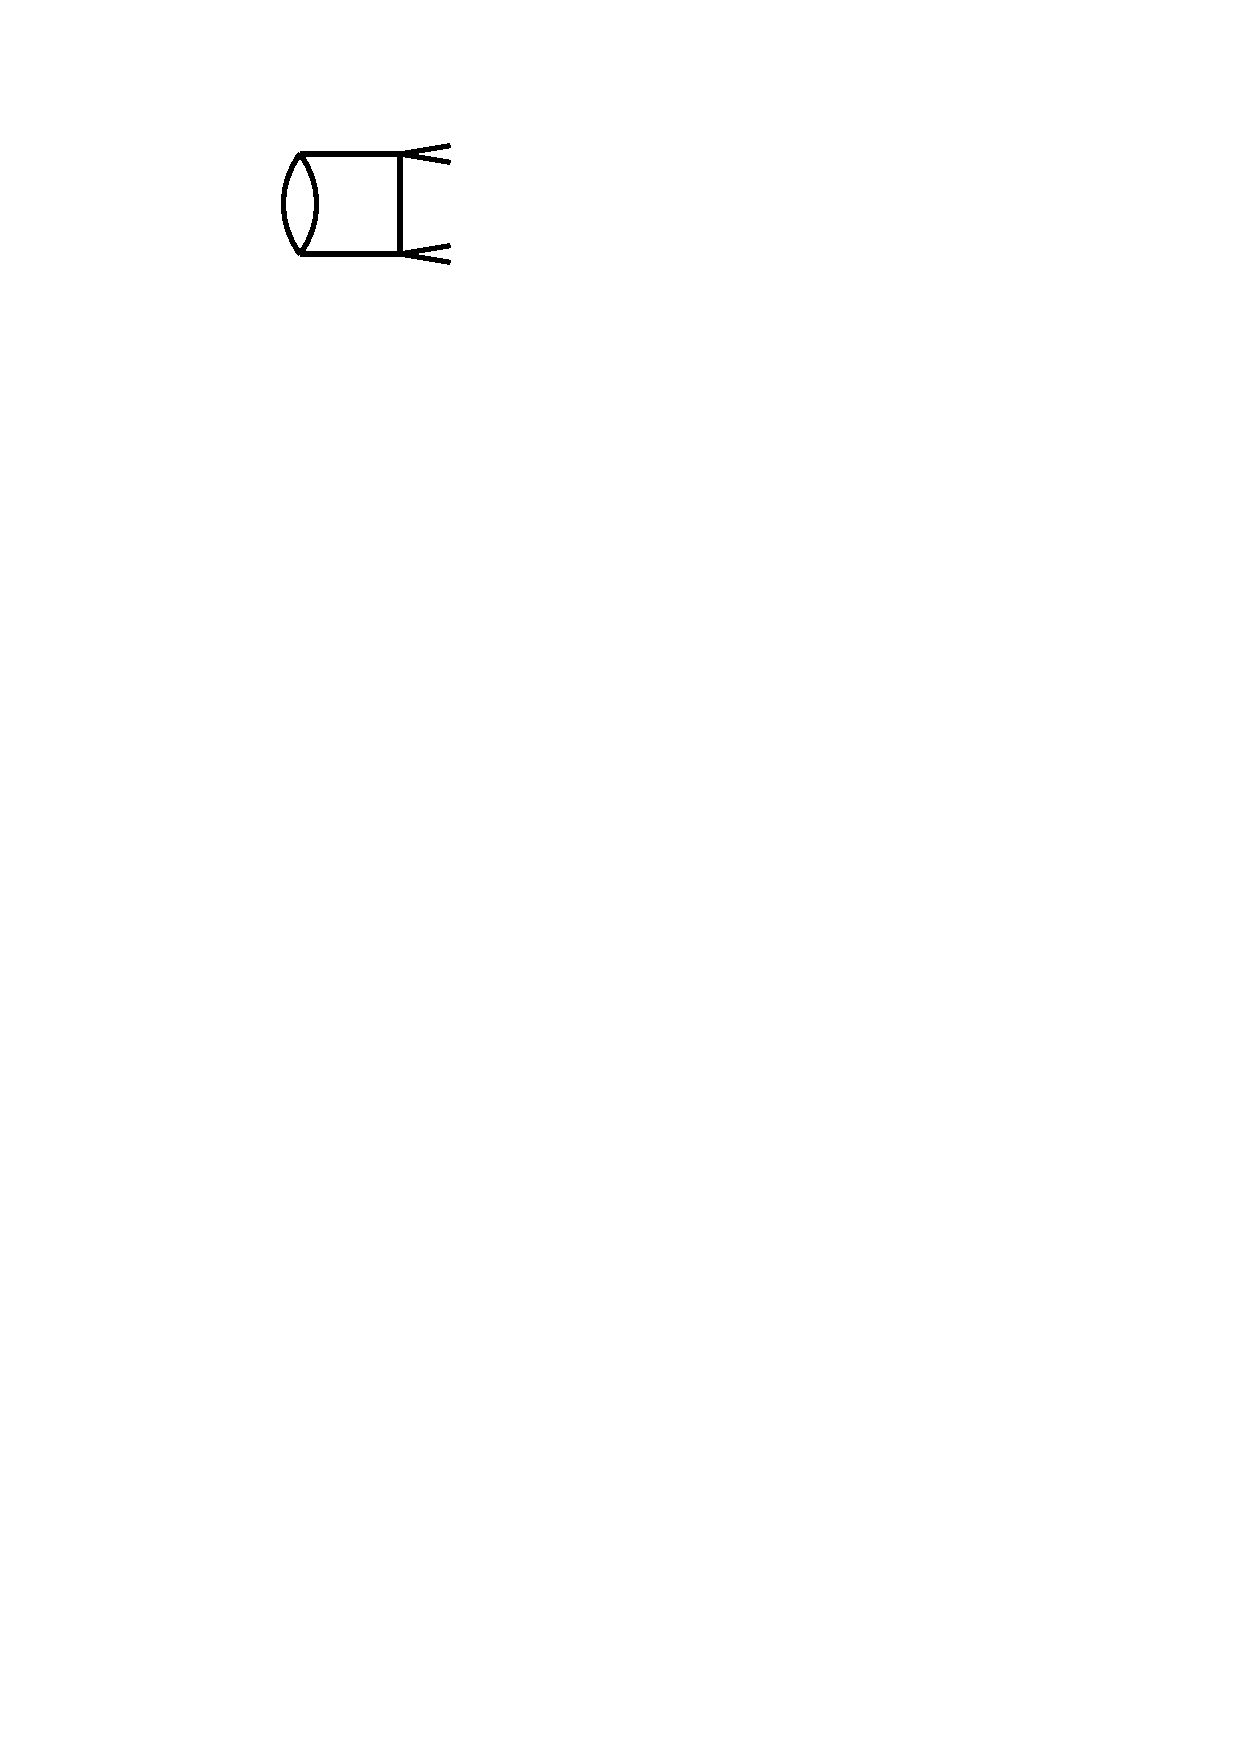
\includegraphics[scale=0.45]{figures/topologies/BoxBubbleRed1}};
      \node at
      (6,-11.5){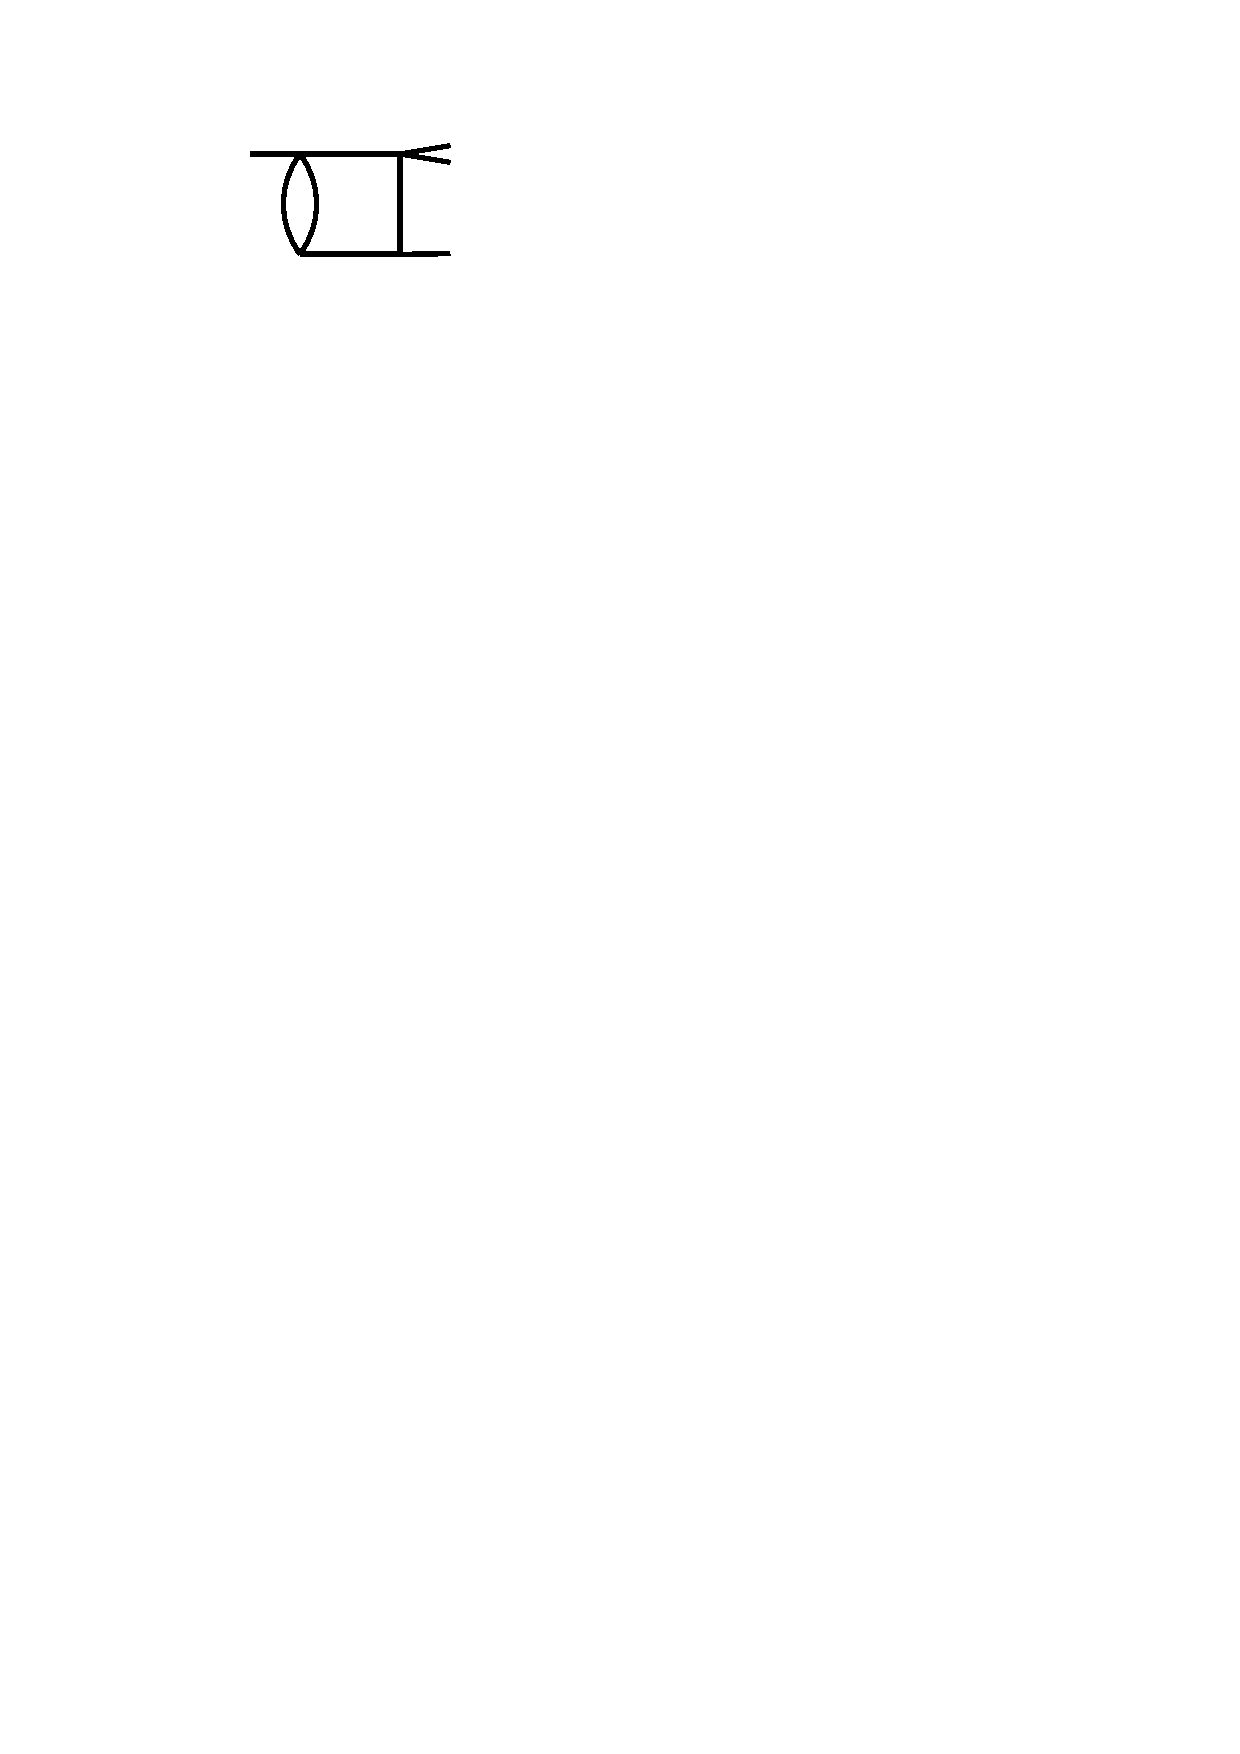
\includegraphics[scale=0.45]{figures/topologies/BoxBubbleRed2}};
      \node at
      (8,-11.5){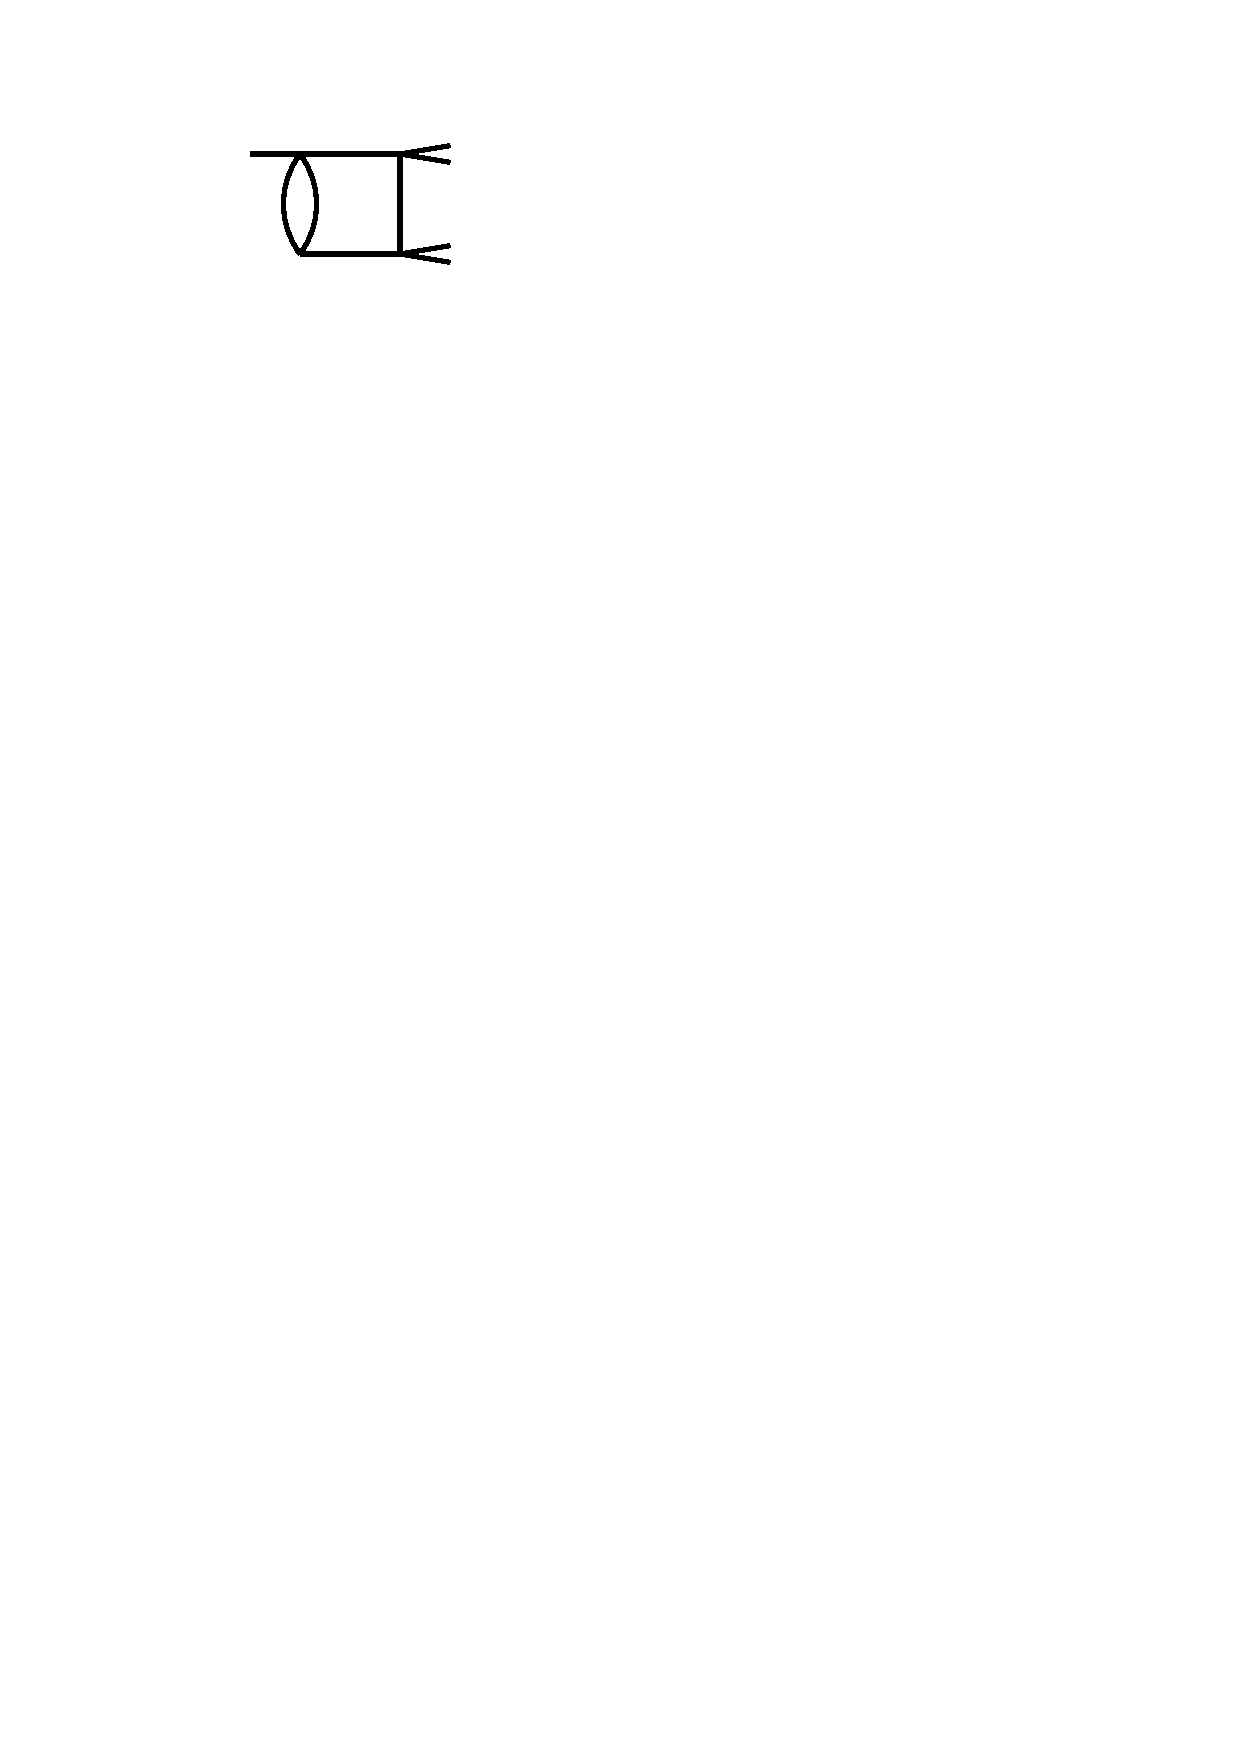
\includegraphics[scale=0.45]{figures/topologies/BoxBubbleRed3}};
      \node at
      (10,-11.5){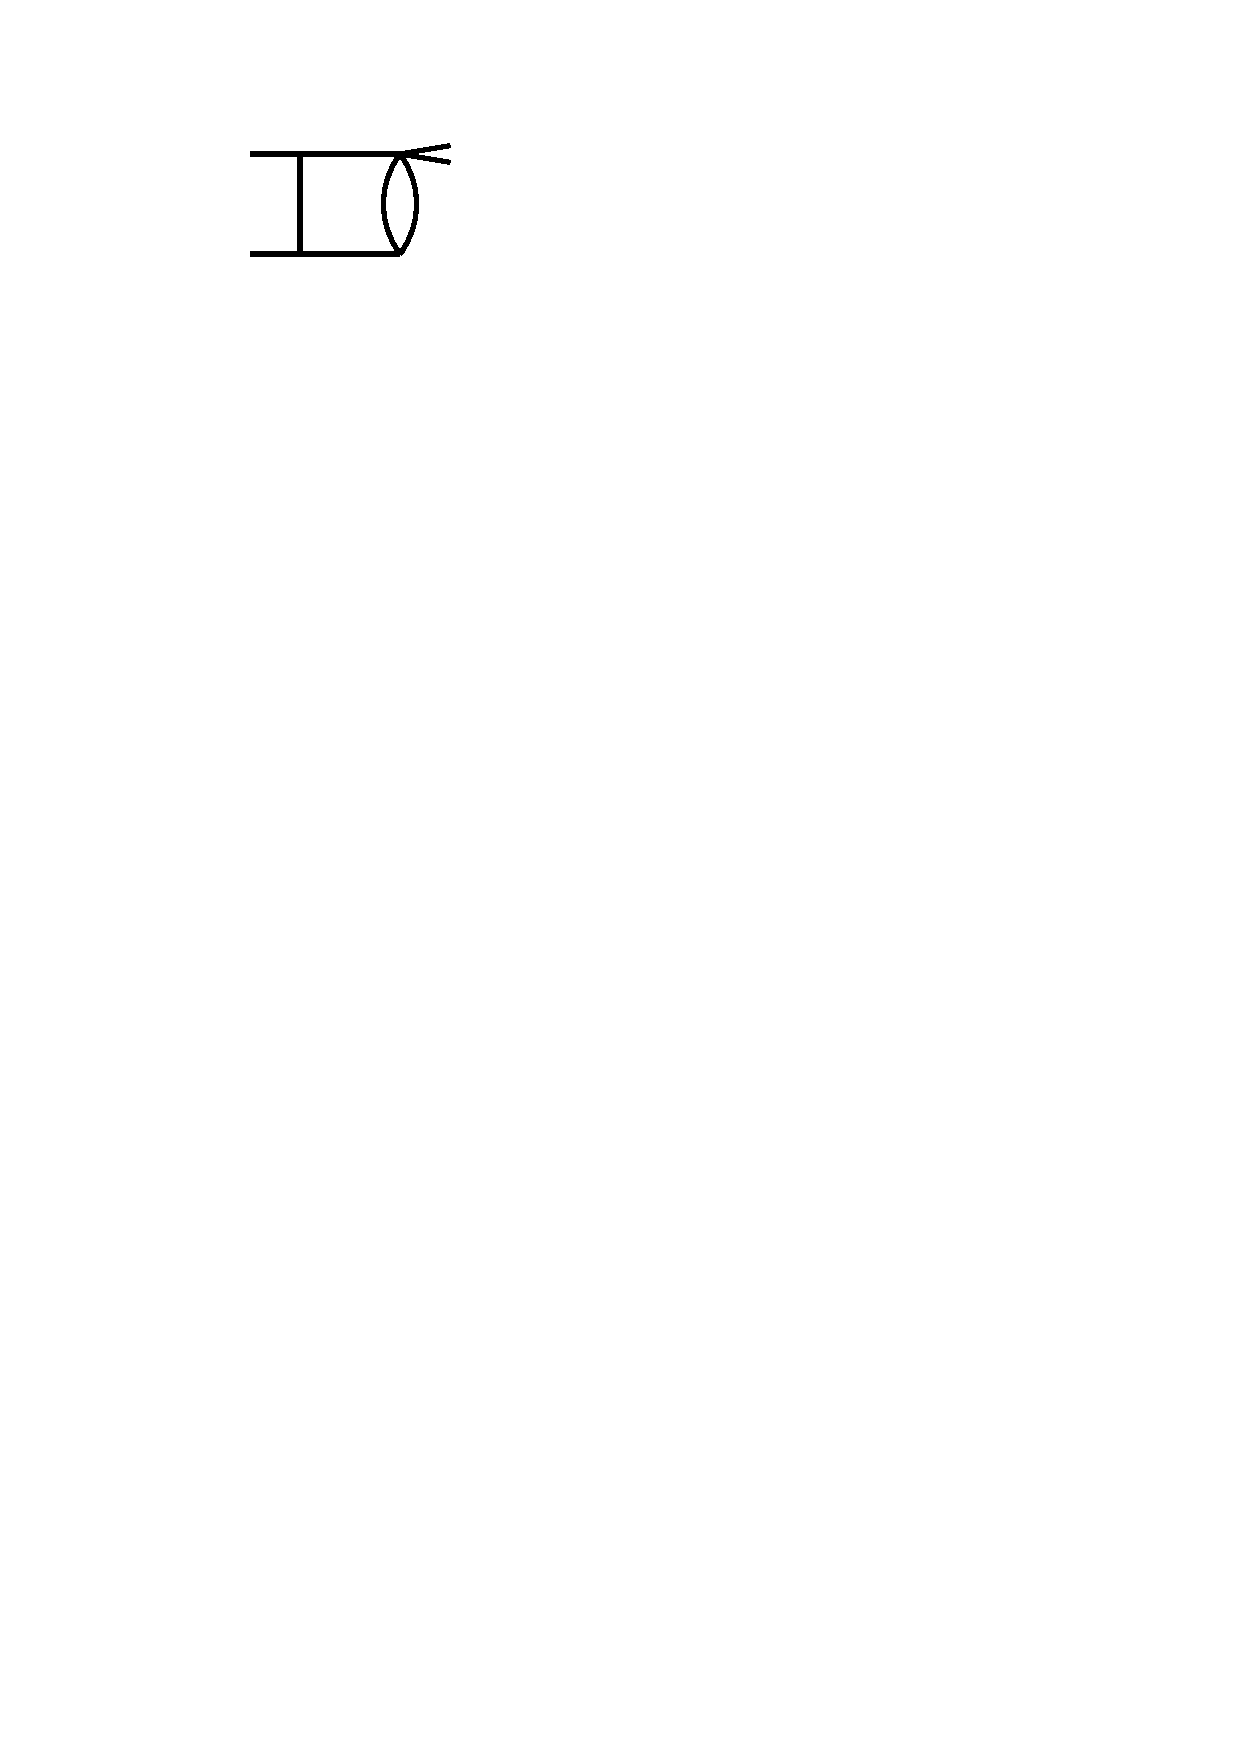
\includegraphics[scale=0.45]{figures/topologies/BoxBubbleRed4}};
    %
      \node at
      (0,-12.7){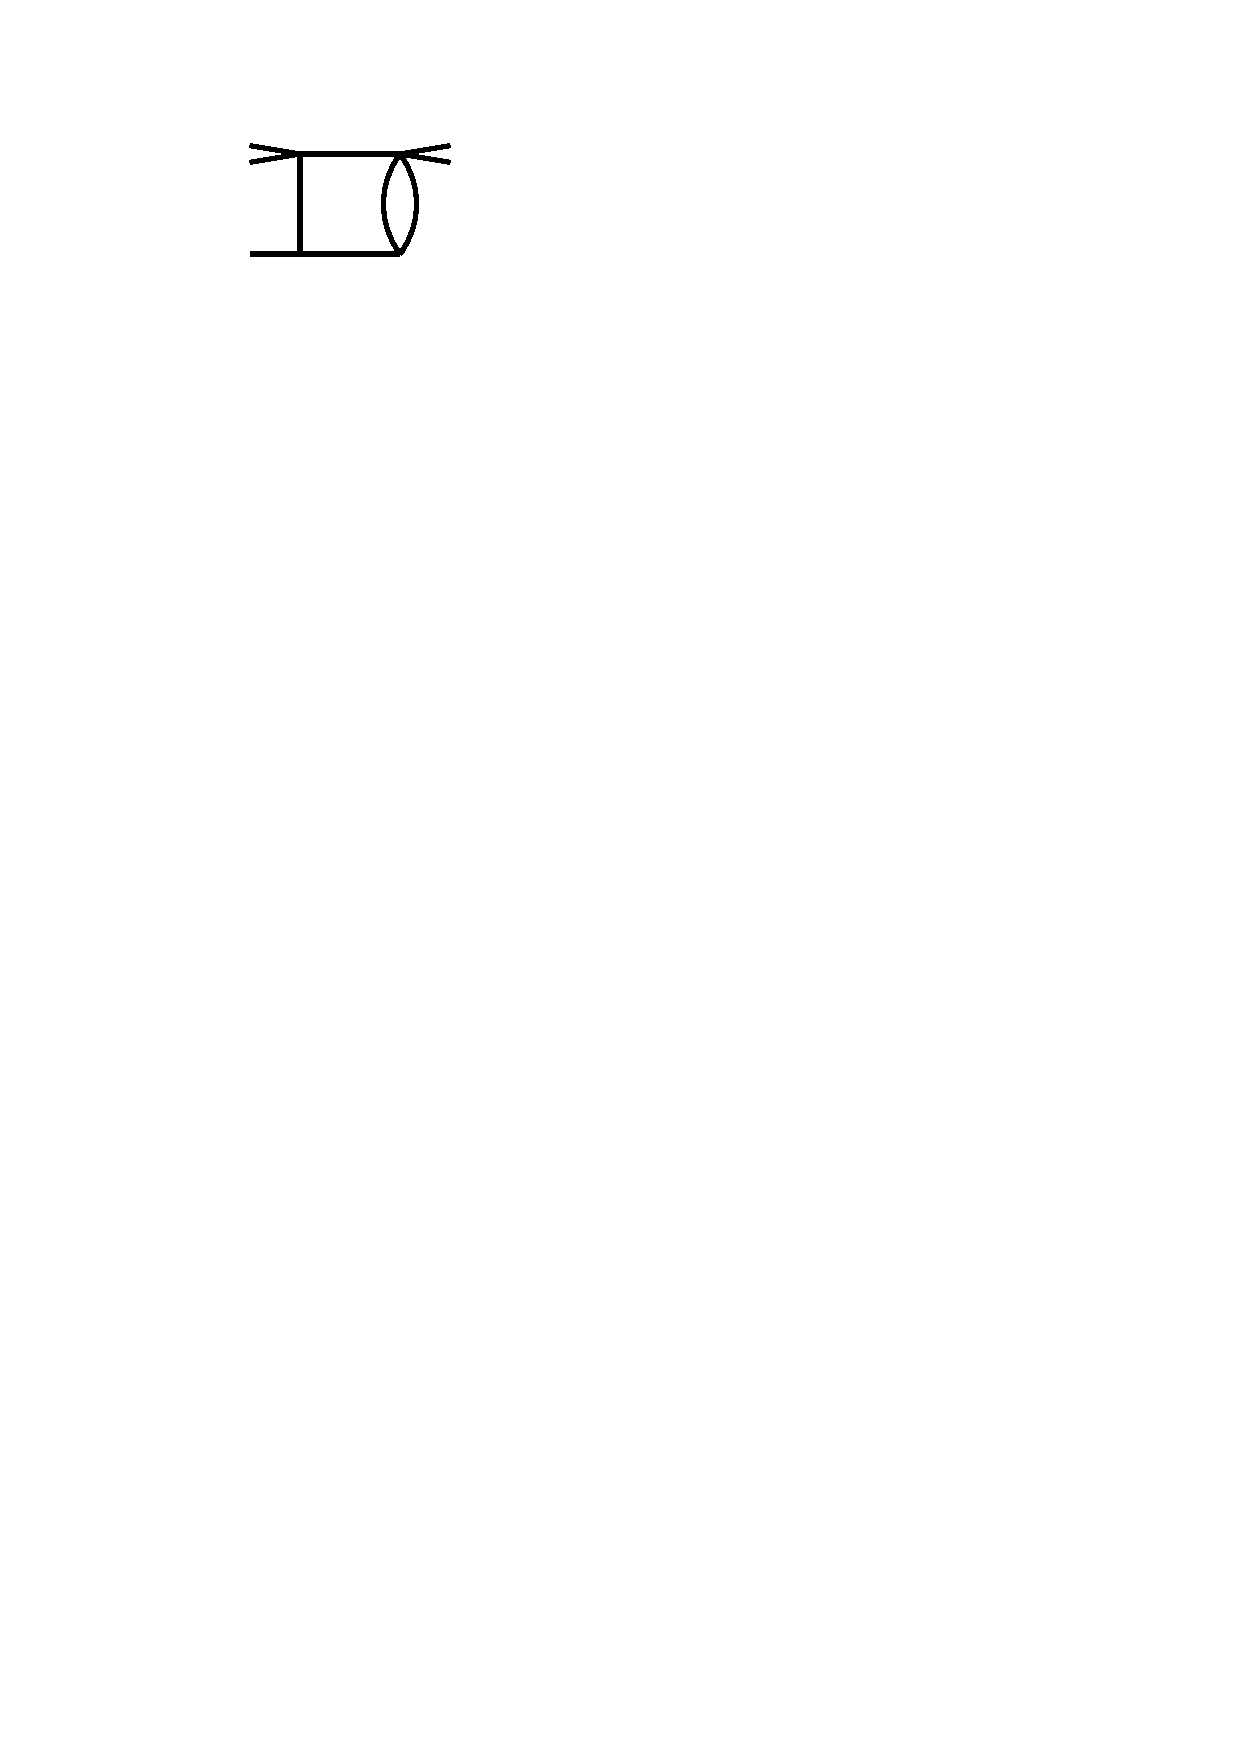
\includegraphics[scale=0.45]{figures/topologies/BoxBubbleRed5}};
      \node at
      (2,-12.7){\includegraphics[scale=0.45]{figures/topologies/BoxBubbleRed6}};
      \node at
      (4,-12.7){\includegraphics[scale=0.45]{figures/topologies/TriangleTriangleGDiag}};
      \node at
      (6,-12.7){\includegraphics[scale=0.45]{figures/topologies/TriangleTriangleGOffDiag}};
      \node at
      (8,-12.6){\includegraphics[scale=0.45]{figures/topologies/TriangleTriangleSG}};
      \node at
      (10.2,-12.75){\includegraphics[scale=0.45] {figures/topologies/TriangleTriangleRed1}};
    %
      \node at
      (0,-13.8){\includegraphics[scale=0.45]{figures/topologies/TriangleTriangleRed2}};
      \node at
      (2.15,-13.8){\includegraphics[scale=0.45] {figures/topologies/TriangleTriangleRed3}};
      \node at
      (4.3,-13.8){\includegraphics[scale=0.45] {figures/topologies/TriangleTriangleRed4}};
      \node at
      (6.45,-13.95){\includegraphics[scale=0.4] {figures/topologies/BubbleTriangle1LS}};
      \node at
      (8.6,-13.95){\includegraphics[scale=0.4] {figures/topologies/BubbleTriangle1LS_2}};
      \node at
      (10.75,-13.95){\includegraphics[scale=0.4] {figures/topologies/BubbleTriangle1LSG}};
    % Level 6
      \node at
      (0,-15.5){\includegraphics[scale=0.5]{figures/topologies/BubbleTriangleG1Mass}};
      \node at
      (1.8,-15.5){\includegraphics[scale=0.5]{figures/topologies/BubbleTriangleG2Mass}};
      \node at
      (3.6,-15.5){\includegraphics[scale=0.5]{figures/topologies/BubbleTriangleSG}};
      \node at
      (5.4,-15.5){\includegraphics[scale=0.5]{figures/topologies/BubbleTriangleRed1}};
      \node at
      (7.2,-15.5){\includegraphics[scale=0.5]{figures/topologies/BubbleTriangleRed2}};
      \node at
      (9,-15.55){\includegraphics[scale=0.5]{figures/topologies/BubbleBubble1LS}};
      \node at
      (10.8,-15.5){\includegraphics[scale=0.5]{figures/topologies/BubbleBubble1LS_2}};
     % Level 7
      \node at
      (5.25,-17){\includegraphics[scale=0.6]{figures/topologies/Sunrise}};
    \end{tikzpicture}
  \end{center}
  \caption{Hierarchy of topologies for two-loop five-parton scattering.
    Only topologically inequivalent structures are shown. All lines
  are massless, with massive external legs being denoted by two massless external lines entering a vertex.}
  \label{fig:PropagatorStructures}
\end{figure}
%%%%%%%%%%%%%%%%%%%%%%%%%%%%

%%%%%%%%%%%%% FIGURE %%%%%%%%%%%%%%%%%%
\begin{figure}[ht] 
  \begin{center}
    \begin{tikzpicture}[scale=1.2]
    % 5 point masters
      \node at (5,0){\includegraphics[scale=0.4]{figures/topologies/BoxPentagon}};
      \node at (5,-1){3 masters};
    % Level 2 
      \node at
      (2.5,-1.5){\includegraphics[scale=0.4]{figures/topologies/BoxBoxSG}};
      \node at (2.5,-2.3){3 masters};
      \node at
      (7.5,-1.6){\includegraphics[scale=0.4]{figures/topologies/BoxBox}};
      \node at (7.5,-2.3){2 masters};
    % Level 3
      \node at
      (0.5,-3.3){\includegraphics[scale=0.35]{figures/topologies/BubblePentagonG}};
      \node at (0.5,-4.1){2 masters};
      \node at
      (3.5,-3.3){\includegraphics[scale=0.4]{figures/topologies/BoxTriangleG}};
      \node at (3.5,-4.1){2 masters};
      \node at
      (6.5,-3.2){\includegraphics[scale=0.4]{figures/topologies/BoxTriangleSG}};
      \node at (6.5,-4.1){1 master};
      \node at
      (9.5,-3.3){\includegraphics[scale=0.4]{figures/topologies/BoxBubble1LS}};
      \node at (9.5,-4.1){1 master};
    % Level 4
      \node at
      (0,-4.9){\includegraphics[scale=0.45]{figures/topologies/BoxBubbleGBox}};
      \node at (0,-5.7){1 master};
      \node at
      (2.5,-4.9){\includegraphics[scale=0.45]{figures/topologies/BoxBubbleGBub}};
      \node at (2.5,-5.7){1 master};
      \node at
      (5,-4.9){\includegraphics[scale=0.45]{figures/topologies/TriangleTriangleGDiag}};
      \node at (5,-5.7){1 master};
      \node at
      (7.5,-4.9){\includegraphics[scale=0.45]{figures/topologies/TriangleTriangleGOffDiag}};
      \node at (7.5,-5.7){2 masters};
      \node at
      (10,-4.8){\includegraphics[scale=0.45]{figures/topologies/TriangleTriangleSG}};
      \node at (10,-5.6){1 master};
    % Level 6
      \node at
      (0.5,-6.5){\includegraphics[scale=0.5]{figures/topologies/BubbleTriangleG1Mass}};
      \node at (0.5,-7.3){1 master};
      \node at
      (3.5,-6.5){\includegraphics[scale=0.5]{figures/topologies/BubbleTriangleG2Mass}};
      \node at (3.5,-7.3){1 master};
      \node at
      (6.5,-6.5){\includegraphics[scale=0.5]{figures/topologies/BubbleBubble1LS}};
      \node at (6.5,-7.3){1 master};
      \node at
      (9.5,-6.45){\includegraphics[scale=0.5]{figures/topologies/BubbleBubble1LS_2}};
      \node at (9.5,-7.2){1 master};
     % Level 7
      \node at
      (5,-8.2){\includegraphics[scale=0.6]{figures/topologies/Sunrise}};
      \node at (5,-9){1 master};
    \end{tikzpicture}
  \end{center}
  \caption{Topologies with master integrals}
  \label{fig:MasterInt}
\end{figure}

\todo{reference \ref{fig:MasterInt} and \ref{fig:PropagatorStructures} from text}

\subsection{Tensors}


\section{Divergence Structure}
\label{sec:IR}

We use the HV dimensional regularization
scheme to handle both ultraviolet and infrared divergences.
UV divergences are removed through renormalization and the
remaining infrared poles can be computed from the corresponding
lower-order
amplitudes~\cite{Catani:1998bh,Sterman:2002qn,Becher:2009cu,
Gardi:2009qi}. In this appendix we detail this procedure.
Reproducing the pole structure of the amplitudes we have 
computed is an important check of our results.


\subsection{Renormalization}

We perform renormalization of the QCD coupling in the 
$\overline{\text{MS}}$ scheme. It is implemented by replacing 
the bare coupling by the renormalized one, denoted $\alpha_s$, 
in eq.~\eqref{eq:partials}.
The bare and renormalized couplings are related through
\begin{equation}\label{eq:renormCoupling}
    \alpha_0\mu_0^{2\epsilon}S_{\epsilon}
  =\alpha_s\mu^{2\epsilon}\left(
  1-\frac{\beta_0}{\epsilon}\frac{\alpha_s}{4\pi}
  +\left(\frac{\beta_0^2}{\epsilon^2}-\frac{\beta_1}{\epsilon}\right)
  \left(\frac{\alpha_s}{4\pi}\right)^2+\mathcal{O}
  \left(\alpha_s^3\right)\right),
\end{equation}
where $S_\epsilon=(4\pi)^{\eps}e^{-\eps\gamma_E}$, with
$\gamma_E=-\Gamma'(1)$ the Euler-Mascheroni constant.
$\mu_0^2$ is the scale introduced in dimensional regularization
to keep the coupling dimensionless in the QCD Lagrangian, 
and $\mu^2$ is the renormalization scale. In the following, we
set $\mu_0^2=\mu^2=1$. The leading-color coefficients of the QCD
$\beta$-function are
\begin{equation}
  \beta_0=\frac{\NC}{3} \left( 11 - 2\frac{N_f}{\NC}
  \right),\qquad
  \beta_1=\frac{\NC^2}{3} \left( 17 - \frac{13}{2} \frac{N_f}{\NC} \right).
\end{equation}
The perturbative expansion of the renormalized amplitude is
\begin{equation}\label{eq:renormAmp}
  \mathcal{A}_R = S_\epsilon^{-\frac{\lambda}{2}}
  g_s^\lambda\left(
  \mathcal{A}_R^{(0)}
  +\frac{\alpha_s}{4\pi}\NC\,\mathcal{A}_R^{(1)}
  +\left(\frac{\alpha_s}{4\pi}\right)^2\NC^2\mathcal{A}_R^{(2)}
  +\mathcal{O}(\alpha_s^3)
  \right),
\end{equation}
where $\lambda$ is the power of $g_0$ in the tree amplitude, 
with $\alpha_0=g_0^2/(4\pi)$ and similarly for $\alpha_s$.
For four-parton amplitudes $\lambda=2$, and for five-parton 
amplitudes $\lambda=3$.
The renormalized amplitudes $\mathcal{A}_R^{(i)}$ are related 
to the bare amplitudes $\mathcal{A}^{(i)}$ as follows:
\begin{align}
  \begin{split}
    \label{eq:twoLoopUnRenorm}
    &\mathcal{A}_R^{(0)}=\mathcal{A}^{(0)}, \\
    & \mathcal{A}_R^{(1)}=S_{\epsilon}^{-1}\mathcal{A}^{(1)}
    -\frac{\lambda}{2\epsilon}\frac{\beta_0}{\NC}
    \mathcal{A}^{(0)}\,,\\
    &\mathcal{A}_R^{(2)}=
    S_{\epsilon}^{-2}\mathcal{A}^{(2)}
    -\frac{\lambda+2}{2\epsilon}\frac{\beta_0}{\NC}S_{\epsilon}^
    {-1}
    \mathcal{A}^{(1)}
    +\left(\frac{\lambda(\lambda+2)}{8\epsilon^2}\left(\frac{\beta_0}
    {\NC}\right)^2
    -\frac{\lambda}{2\epsilon}\frac{\beta_1}{\NC^2}\right)
    \mathcal{A}^{
    (0)}\,.
  \end{split}
\end{align}



\subsection{Infrared Behavior}

The poles of renormalized amplitudes are of infrared origin and
can be predicted from the previous orders in the perturbative 
expansion 
\cite{Catani:1998bh,Sterman:2002qn,Becher:2009cu,Gardi:2009qi}:
\begin{align}
  \begin{split}\label{eq:catani}
    A_R^{(1)}&=\mathbf{I}^{(1)}_{[n]}(\epsilon)
    A_R^{(0)}+\mathcal{O}
    (\epsilon^0)\,,\\
    A_R^{(2)}&=\mathbf{I}^{(2)}_{[n]}(\epsilon)A_R^{(0)}+\mathbf{I}^{(1)}_{[n]}(\epsilon)
    A_R^{(1)}+\mathcal{O}(\epsilon^0)\,,
  \end{split}
\end{align}
with the operators $\mathbf{I}^{(1)}_{[n]}$ and
$\mathbf{I}^{(2)}_{[n]}$ depending on the number and the type of
the scattering particles. This dependence is denoted by the 
subscript $[n]$.
For amplitudes in the leading-color approximation and for which
all quark lines have distinct flavor, the operators
$\mathbf{I}^{(1)}_{[n]}$ and $\mathbf{I}^{(2)}_{[n]}$ are 
diagonal in color space and can be written in a very compact
form. The operator $\mathbf{I}^{(1)}_{[n]}$ is given by
%
\begin{equation}
  \mathbf{I}^{(1)}_{[n]}(\eps)=-\frac{e^{\gamma_E\eps}}{\Gamma(1-\epsilon)}
  \sum_{i=1}^n\gamma_{a_i,a_{i+1}}
  \left( -s_{i,i+1}\right)^{-\epsilon}\,,
\end{equation}
with the indices defined cyclically.
The index $a_i$ denotes a type of particle with momentum $p_i$, i.e., in the context of our paper,
$a_i\in\{g,q,\bar q, Q, \bar Q\}$. We introduced the auxiliary symbols $\gamma_{a,b}$, 
symmetric under the exchange of indices, 
$\gamma_{a,b}=\gamma_{b,a}$, and defined according to:
\begin{align}
  \begin{split}
    \gamma_{g,g}&=\frac{1}{\epsilon^2}+\frac{1}{2\eps}
    \frac{\beta_0}{\NC}\,, \\
    \gamma_{q,Q}&=\gamma_{q,\bar Q}=
    \gamma_{\bar q, Q}=\gamma_{\bar q, \bar Q} 
    =\frac{1}{\epsilon^2}+\frac{3}{2\eps}\,,\\
    \gamma_{g,q}&=\gamma_{g,\bar q}=
    \gamma_{g,Q}=\gamma_{g,\bar Q}=
    \frac{\gamma_{g,g}+\gamma_{q,Q}}{2}\,,\\
    \gamma_{q,\bar q}&=\gamma_{Q,\bar Q}=0\,.
  \end{split}
\end{align}
The operator~$\mathbf{I}^{(2)}_{[n]}$ is
\begin{align}
  \label{eqn:Iop}
  \begin{split} 
    \mathbf{I}^{(2)}_{[n]}(\eps)=&
    -\frac{1}{2}\mathbf{I}^{(1)}_{[n]}(\eps)\mathbf{I}^{(1)}_{[n]}(\eps)
    -\frac{\beta_0}{\NC\epsilon}\mathbf{I}^{(1)}_{[n]}(\eps) + 
    \frac{e^{-\gamma_E\epsilon}\Gamma(1-2\epsilon)}
    {\Gamma(1-\epsilon)}
    \left(\frac{\beta_0}{\NC\epsilon}+K\right)
    \mathbf{I}^{(1)}_{[n]}(2\epsilon) + 
    \mathbf{H}_{[n]}(\epsilon)\,,
  \end{split}
\end{align}
where 
\begin{equation}
K=\frac{67}{9}-\frac{\pi ^2}{3}-\frac{10}{9}\frac{\NF}{\NC}\,,
\end{equation}
and $\mathbf{H}_{[n]}(\epsilon)$ is a diagonal operator at 
leading color that depends on the number of external quarks 
and gluons in the process,
\begin{align}
  \begin{split}
    \mathbf{H}_{[n]}(\epsilon)&=
    \frac{e^{\gamma_E\epsilon}}{\epsilon\Gamma(1-\epsilon)}
    \sum_{i=1}^n\left(
    \delta_{a_i,g}H_g+
    (\delta_{a_i,q}+\delta_{a_i,\bar q}
    +\delta_{a_i,Q}+\delta_{a_i,\bar Q})
    H_q
    \right)\,,
  \end{split}
\end{align}
with (see e.g.~\cite{Bern:2003ck})
\begin{align}
  \begin{split}
    H_g&= \left(\frac{\zeta_3}{2}+\frac{5}{12}+
    \frac{11\pi^2}{144}\right)
    -\left(\frac{\pi^2}{72}+\frac{89}{108}\right)\frac{N_f}{\NC}
    +\frac{5}{27}\left(\frac{N_f}{\NC}\right)^2\,,\\
    H_q&=
    \left(\frac{7\zeta_3}{4}+\frac{409}{864}
    -\frac{11\pi^2}{96}\right)
    +\left(\frac{\pi^2}{48}-\frac{25}{216}\right)\frac{N_f}{\NC}\,.
  \end{split}
\end{align}

The poles of the bare amplitudes, as presented for example in
tables~\ref{tab:results4parton} and \ref{tab:results5parton}, can be recovered
from those of the renormalized amplitude by using
eqs.~\eqref{eq:twoLoopUnRenorm}.

\subsection{Finite Remainder}\label{sec:remainders}

As we have seen above,
the bare scattering amplitudes defined in eq.~\eqref{eq:nfdecomposition}
have divergences of ultraviolet and infrared origin which can be predicted from lower orders in perturbation theory.
It is convenient to remove this redundant information and define a \emph{finite remainder} that contains the new two-loop information.
If one is concerned only about removing the divergences a definition of the remainder is not unique, so we now discuss our conventions.

%The renormalized amplitudes can be obtained from their bare counterparts
%by replacing in eq.~\eqref{eq:partials} the bare QCD coupling $\alpha_0$
%by the renormalized coupling $\alpha_s$ in $D=4-2\epsilon$ dimensions. 
%The two couplings are related by
%which we can use to define the perturbative expansion of the renormalized
%amplitude,
%\begin{equation}\label{eq:renormAmp}
  %\mathcal{A}_R = S_\epsilon^{-\frac{3}{2}}
  %g_s^3\left(
  %\mathcal{A}_R^{(0)}
  %+\frac{\alpha_s}{4\pi}\NC\,\mathcal{A}_R^{(1)}
  %+\left(\frac{\alpha_s}{4\pi}\right)^2\NC^2\mathcal{A}_R^{(2)}
  %+\mathcal{O}(\alpha_s^3)
  %\right),
%\end{equation}
%where $S_\epsilon=(4\pi)^{\epsilon}e^{-\epsilon\gamma_E}\,$ and 
%$\alpha_s=g_s^2/(4\pi)$. The $\beta_i$ are the coefficients in the
%perturbative expansion of the QCD $\beta$-function, which we give explicitly
%in appendix \ref{app:remainderDetails}. 
%Here, $\mu_0^2$ is the scale introduced in dimensional regularization to keep the
%coupling dimensionless in the QCD Lagrangian, and $\mu^2$ is the
%renormalization scale. In the following, we set $\mu^2=\mu_0^2=1$ (with arbitrary dimensions).

%The renormalized amplitudes $\CA^{(k)}_R$ have only infrared divergences,
%which can be determined from lower-loop functions and well known universal 
%factors \cite{Catani:1998bh,Sterman:2002qn,Becher:2009cu,Gardi:2009qi}. More
%precisely, we have
%\begin{align}\begin{split}\label{eq:catani}
    %\CA_R^{(1)}&=\mathbf{I}^{(1)}_{[n]}(\epsilon)
    %\CA_R^{(0)}+\mathcal{O}
    %(\epsilon^0)\,,\\
    %\CA_R^{(2)}&=\mathbf{I}^{(2)}_{[n]}(\epsilon)\CA_R^{(0)}+\mathbf{I}^{(1)}_{[n]}(\epsilon)
    %\CA_R^{(1)}+\mathcal{O}(\epsilon^0)\,.
%\end{split}\end{align}
%The $\mathbf{I}^{(k)}_{[n]}$ are operators in color space that become diagonal
%in the leading-color approximation. They contain some
%process-specific components, and explicit expressions are given 
%in appendix~\ref{app:remainderDetails}.

Using \cref{eq:renormCoupling,eq:renormAmp,eq:catani}, we can predict
the poles of the two-loop amplitudes we wish to compute. Alternatively, we
can use them to define a finite remainder $\mathcal{R}^{(2)}$, according to
\begin{equation}\label{eq:remaindeDef}
  \mathcal{R}^{(2)}=\mathcal{A}_R^{(2)}
  -\mathbf{I}_{[n]}^{(1)}\mathcal{A}_R^{(1)}
  -\mathbf{I}_{[n]}^{(2)}\mathcal{A}_R^{(0)}
  +\mathcal{O}(\epsilon)\,.
\end{equation}
Here we expand one-loop amplitudes $\mathcal{A}_R^{(1)}$ to order $\eps^2$ to capture the terms of order $\eps^0$
from the cancellation with the corresponding $\frac{1}{\eps^2}$ pole in the operator $\mathbf{I}_{[n]}^{(1)}$.

This subtracts non-trivial contributions from
the finite term of $\mathcal{A}_R^{(2)}$ that are related to 
the lower-loop amplitudes.
In section \ref{sec:AnalyticForm} we will obtain analytic expression for the finite remainder directly.
If necessary one can then recover the two-loop bare amplitude $\CA^{(2)}$ by inverting
the relations \eqref{eq:twoLoopUnRenorm}:
\begin{align}
  \begin{split}
    \label{eq:ampFromRem}
    {\mathcal{A}}^{(2)}=&\,\mathcal{R}^{(2)}+
    S_\epsilon{\mathcal{A}}^{(1)}
    \left(\mathbf{I}_{[n]}^{(1)}+\frac{5}{2\epsilon}
    \frac{\beta_0}
    {N_c}\right)\\
    &-S_\epsilon^2 {\mathcal{A}}^{(0)}
    \left(
    \frac{15}{8\epsilon^2}
    \left(\frac{\beta_0}{N_c}\right)^2+\frac{3}{2\epsilon}
    \left(\frac{\beta_0}{N_c}\mathbf{I}_{[n]}^{(1)}-
    \frac{\beta_1}{N_c^2}\right)-\mathbf{I}_{[n]}^{(2)}
    \right)+\mathcal{O}(\epsilon)\,.
  \end{split}
\end{align}

\todo{possibly here section ``Implementation Details''}


\section{Validation}
\label{sec:Validation-5parton}
\todo{restructure and add some missing items}

We have validated our results by carrying out a set of
checks. We verified that they satisfy the
expected infrared pole structure \cite{Catani:1998bh}. We summarize the
relevant formulae for this check in \cref{sec:IR}.
Furthermore, we have carried out a systematic
validation of the $\epsilon^0$ contributions of all of 
our results against their known analytic
expressions from refs.~\cite{Bern:2002tk,Bern:2003ck,
DeFreitas:2004kmi,Glover:2004si}. 
For the four-gluon amplitudes we have compared directly the
$\epsilon^0$ pieces of our results with the analytic expressions
of~\cite{Bern:2002tk}.

For the two-quark two-gluon and four-quark amplitudes we have used the one-loop results given in \cref{tab:results4parton1L}
to compute the corresponding finite remainders $\CF^{(2)}$ as
defined in \cref{eq:remainderDef}. 
After accounting for the different choices of 
normalization for the $\mathbf{H}_{[n]}(\epsilon)$ operators 
(see \cref{sec:IR})
made in refs.~\cite{Bern:2003ck} and \cite{Glover:2004si},
we have found perfect agreement.

\section{Numerical Results}

Here provide details of how numerical evaluation has been performed.

Floating point and finite fields coefficients.
Cite numerical libraries qd and givaro.

Different sources for integrals: PTW, based on pentagon functions in Caravel.



Once the coefficients $c_{\Gamma,i}$ in \cref{eq:AL} are computed,
we obtain a decomposition of the amplitude into master integrals,
\begin{equation}
  \mathcal{A}^{(2)}=\sum_{\Gamma\in\Delta}
  \sum_{i\in M_\Gamma} c_{\Gamma,i}\,
  \mathcal{I}_{\Gamma,i}\,,
  \label{eq:Amaster}
\end{equation}
where the $\mathcal{I}_{\Gamma,i}$ are the master integrals,
\begin{equation}
  \mathcal{I}_{\Gamma,i}=\int d^D\ell_l
  \frac{m_{\Gamma,i}(\ell_l)}
  {\prod_{j\in P_\Gamma}\rho_j}\,.
\end{equation}
For planar five-parton amplitudes, a basis of master integrals has been 
computed~\cite{Papadopoulos:2015jft,Gehrmann:2018yef}.
The master integrals evaluate to linear combinations of so-called 
multiple polylogarithms (MPLs), which can be 
numerically evaluated using available programs 
(e.g.~\cite{Vollinga:2004sn}). Once numerical values for the coefficients 
$c_{\Gamma,i}$ have been  computed (using for example 
the approach described in the previous subsection) one can obtain numerical values
for the amplitudes.


\subsection{One-Loop}

One-loop amplitudes were known. Five-parton to order $\mathcal{O}(\eps^2)$ are presented for the first time.

\begin{table}[h]
  \centering
  \begin{adjustbox}{width=1\textwidth}
    \begin{tabular}{cccccc}
      \toprule
      $\CA^{(1)[N_f^0]}/\CA^\mathrm{(norm)}$   &   $\epsilon^{-2}$   &   $\epsilon^{-1}$   &   $\epsilon^{0}$   &   $\epsilon^{1}$  &  $\epsilon^{2}$ \\
      \midrule
      $(1_g^+,2_g^+,3_g^+,4_g^+)$ & $0$ & $0$ & $1$ & 
      $3.144383516$
      & $4.993655130$ \\
      $(1_g^-,2_g^+,3_g^+,4_g^+)$ & $0$ & $0$ & $1$ & 
      $6.037021519$
      & $19.41121185$ \\
      $(1_g^-,2_g^-,3_g^+,4_g^+)$ &  $-4.000000000$ &
      $-14.82985386$ &
      $-21.50563510$ & $-4.242972632$ & $39.45669987$ \\
      $(1_g^-,2_g^+,3_g^-,4_g^+)$ &  $-4.000000000$ &
      $-14.82985386$ & $-24.34737636$ & $-23.80446527$ &
      $-30.91926414$\\ \midrule
      $(1_q^+,2_{\bar q}^-,3_g^+,4_g^+)$ & $0$ & $0$ & $1$ &
      $5.886473216$  & $18.18093693$   \\
      $(1_q^+,2_{\bar q}^-,3_g^+,4_g^-)$ & $-3.000000000$ &
      $-10.42169654$ & $-13.75537910$ & $-2.227311547$ &
      $15.67564907$ \\
      $(1_q^+,2_{\bar q}^-,3_g^-,4_g^+)$ & $-3.000000000$ &
      $-10.42169654$ &
      $-10.64041688$ & $20.52306512$ & $101.8467214$ \\
      \midrule
      $(1_q^+,2_{\bar q}^-,3_Q^-,4_{\bar Q}^+)$ & $-2.000000000$ &
      $-6.013539220$  & $4.503971305$ & $55.27734017$ &
      $156.3375209$ \\
      $(1_q^+,2_{\bar q}^-,3_Q^+,4_{\bar Q}^-)$ & $-2.000000000$ &
      $-6.013539220$  & $-1.512122300$ & $22.96961380$ &
      $57.55706218$ \\
      \toprule
      $\CA^{(1)[N_f^1]}/\CA^\mathrm{(norm)}$   &   $\epsilon^{-2}$   &   $\epsilon^{-1}$   &   $\epsilon^{0}$   &   $\epsilon^{1}$  &  $\epsilon^{2}$ \\
      \midrule
      $(1_g^+,2_g^+,3_g^+,4_g^+)$ & $0$ & $0$ & $-1.000000000$ &
      $-4.144383516$ & $-9.138038646$\\
      $(1_g^-,2_g^+,3_g^+,4_g^+)$ & $0$ & $0$ & $-1.000000000$ &
      $-7.037021519$ & $-26.44823337$ \\
      $(1_g^-,2_g^-,3_g^+,4_g^+)$ & $0$ & $0.6666666667$ &
      $3.337846407$ & $7.778113386$ & $9.642499788$ \\
      $(1_g^-,2_g^+,3_g^-,4_g^+)$ & $0$ & $0.6666666667$ &
      $3.888266255$ & $11.57993010$ & $23.40355137$ \\
      \midrule
      $(1_q^+,2_{\bar q}^-,3_g^+,4_g^+)$ & $0$ & $0$ &
      $-0.1818181818$ & $-1.074210422$ & $-3.518712119$ \\
      $(1_q^+,2_{\bar q}^-,3_g^+,4_g^-)$ & $0$ & $0$ & $0$ & $0$ & $0$ \\
      $(1_q^+,2_{\bar q}^-,3_g^-,4_g^+)$ & $0$ & $0$ & $0$ & $0$ & $0$ \\
      \midrule
      $(1_q^+,2_{\bar q}^-,3_Q^-,4_{\bar Q}^+)$ & $0$ &
      $-0.6666666667$ & $-2.605438214$ & $-5.691068008$ &
      $-8.728233619$ \\
      $(1_q^+,2_{\bar q}^-,3_Q^+,4_{\bar Q}^-)$ & $0$ &
      $-0.6666666667$ & $-2.605438214$ & $-5.691068008$ &
      $-8.728233619$ \\
      \bottomrule
    \end{tabular}
  \end{adjustbox}
\caption{The bare one-loop four-parton helicity amplitudes 
  evaluated at the phase space point in \cref{eq:EvalPoint4}. We set the
    normalization factor $\CA^\mathrm{(norm)}$ to $\CA^{(1)[N_f^0]}(\epsilon=0)$ for the
    amplitudes with vanishing trees, and to $\CA^{(0)}$ otherwise.}
  \label{tab:results4parton1L}
\end{table}

\begin{table}[h]
  \centering
  \begin{adjustbox}{width=1\textwidth}
    \begin{tabular}{cccccc}
      \toprule
      $\CA^{(1)[N_f^0]}/\CA^\mathrm{(norm)}$   &   $\epsilon^{-2}$   &   $\epsilon^{-1}$   &   $\epsilon^{0}$   &   $\epsilon^{1}$  &  $\epsilon^{2}$ \\
      \midrule
      $(1_g^+,2_g^+,3_g^+,4_g^+,5_g^+)$ & $0$ & $0$ & $1$ &
      $3.033832975$ & $4.587604357$ \\
      $(1_g^-,2_g^+,3_g^+,4_g^+,5_g^+)$ & $0$ & $0$ & $1$ &
      $5.624431423$ & $16.89796219$ \\
      $(1_g^-,2_g^-,3_g^+,4_g^+,5_g^+)$ &  $-5.000000000$ &
      $-17.88291386$ & $-24.30905600$ & $0.2206218531$ &
      $59.35260478$ \\
      $(1_g^-,2_g^+,3_g^-,4_g^+,5_g^+)$ &  $-5.000000000$ &
      $-17.88291386$ & $-29.50855173$ & $-34.92963561$ &
      $-64.50302993$ \\
      \midrule
      $(1_q^+,2_{\bar q}^-,3_g^+,4_g^+,5_g^+)$ & $0$ & $0$ & $1$ &
      $5.892137144$ & $18.35590938$ \\
      $(1_q^+,2_{\bar q}^-,3_g^+,4_g^+,5_g^-)$ & $-4.000000000$ &
      $-13.76243861$ & $-15.50477253$ & $17.23285932$ &
      $101.5375461$ \\
      $(1_q^+,2_{\bar q}^-,3_g^+,4_g^-,5_g^+)$ & $-4.000000000$ &
      $-13.76243861$ & $-17.97203103$ & $1.496892271$ &
      $50.75427433$ \\
      $(1_q^+,2_{\bar q}^-,3_g^-,4_g^+,5_g^+)$ & $-4.000000000$ &
      $-13.76243861$ & $-16.98218729$ & $7.025105072$ &
      $65.53899984$ \\
      \midrule
      $(1_q^+,2_{\bar q}^-,3_Q^-,4_{\bar Q}^+,5_g^+)$ &
      $-3.000000000$& $-8.843501370$ & $-1.852152501$ &
      $37.28945738$
      & $105.9935237$ \\
      $(1_q^+,2_{\bar q}^-,3_Q^+,4_{\bar Q}^-,5_g^+)$ &
      $-3.000000000$& $-8.843501370$ & $-4.411871382$ &
      $26.32328221$ & $81.15715418$ \\
      $(1_q^+,2_{\bar q}^-,3_Q^-,4_{\bar Q}^+,5_g^-)$ &
      $-3.000000000$& $-8.843501370$ & $342.9945174$ &
      $1000.539160$ & $-355.3299610$ \\
      $(1_q^+,2_{\bar q}^-,3_Q^+,4_{\bar Q}^-,5_g^-)$ &
      $-3.000000000$&
      $-8.843501370$ & $-1.744812968$ & $-9.470771643$ &
      $-176.4533405$ \\
      \toprule
      $\CA^{(1)[N_f^1]}/\CA^\mathrm{(norm)}$   &   $\epsilon^{-2}$   &   $\epsilon^{-1}$   &   $\epsilon^{0}$   &   $\epsilon^{1}$  &  $\epsilon^{2}$ \\
      \midrule
      $(1_g^+,2_g^+,3_g^+,4_g^+,5_g^+)$ & $0$ & $0$ &
      $-1.000000000$ & $-4.033832975$ & $-8.621437332$ \\
      $(1_g^-,2_g^+,3_g^+,4_g^+,5_g^+)$ & $0$ & $0$ &
      $-1.000000000$ & $-6.624431423$ & $-23.52239361$ \\
      $(1_g^-,2_g^-,3_g^+,4_g^+,5_g^+)$ &  $0$ & $0.6666666667$ &
      $2.494683591$ & $2.329188091$ & $-8.735477566$ \\
      $(1_g^-,2_g^+,3_g^-,4_g^+,5_g^+)$ &  $0$ & $0.6666666667$ &
      $3.475701080$ &  $8.982161551$ &  $14.85398827$ \\
      \midrule
      $(1_q^+,2_{\bar q}^-,3_g^+,4_g^+,5_g^+)$ & $0$ & $0$ &
      $-0.3542206031$ & $-2.268220888$ & $-7.918667025$ \\
      $(1_q^+,2_{\bar q}^-,3_g^+,4_g^+,5_g^-)$ & $0$ & $0$ &
      $-0.5535785746$ & $-3.637432164$ & $-12.69744845$ \\
      $(1_q^+,2_{\bar q}^-,3_g^+,4_g^-,5_g^+)$ & $0$ & $0$ &
      $-0.0008015520164$ & $-0.004344237791$ & $-0.01257682159$
      \\
      $(1_q^+,2_{\bar q}^-,3_g^-,4_g^+,5_g^+)$ & $0$ & $0$ &
      $-0.04501904941$ & $-0.2962279378$ & $-1.036895298$ \\
      \midrule
      $(1_q^+,2_{\bar q}^-,3_Q^-,4_{\bar Q}^+,5_g^+)$ & $0$ &
      $-0.6666666667$ & $-2.939327989$ & $-7.089932089$ &
      $-11.96893214$ 
      \\
      $(1_q^+,2_{\bar q}^-,3_Q^+,4_{\bar Q}^-,5_g^+)$ & $0$ &
      $-0.6666666667$ & $-2.933154494$ & $-7.055606900$ &
      $-11.86563786$ 
      \\
      $(1_q^+,2_{\bar q}^-,3_Q^-,4_{\bar Q}^+,5_g^-)$ & $0$ &
      $-0.6666666667$ & $-57.49865762$ & $-259.2491530$ &
      $-668.4609808$
      \\
      $(1_q^+,2_{\bar q}^-,3_Q^+,4_{\bar Q}^-,5_g^-)$ & $0$ &
      $-0.6666666667$ & $1.491351996$ & $9.944256190$ & 
      $24.03526126$ \\
      \bottomrule
    \end{tabular}
  \end{adjustbox}
  \caption{The bare one-loop five-parton helicity amplitudes 
  evaluated at the phase space point in \cref{eq:EvalPoint5}. We set the
    normalization factor $\CA^\mathrm{(norm)}$ to $\CA^{(1)[N_f^0]}(\epsilon=0)$ for the
    amplitudes with vanishing trees, and to $\CA^{(0)}$ otherwise.}
  \label{tab:results5parton1L}
\end{table}

\subsection{Four-Parton}

\todo{Move four-parton results to appendix and refer from validation? Or move to validation}

We evaluate the four-gluon, two-quark two-gluon and four-quark
amplitudes at the phase-space point%
\footnote{Units of energy are chosen arbitrarily.
  The amplitudes presented in the tables
  \ref{tab:results4parton}, \ref{tab:results5parton}, 
  \ref{tab:results4parton1L} and \ref{tab:results5parton1L}
  are normalized to be dimensionless.
}
%
\begin{equation}
  \begin{aligned}[c]
    p_1 &= \vphantom{\frac{1}{48}}\left(1,1,-i,1\right), \\
    p_2 &= -\frac{1}{16}\left(3,0,0,-3\right), \\
  \end{aligned}
  \qquad
  \begin{aligned}[c]
    p_3 &= \frac{1}{48}\left(25,-51,45\,i,7\right),\\
    p_4 &= -\frac{1}{48}\left(64,-3,-3\,i, 64\right), \\
  \end{aligned}
  \label{eq:EvalPoint4}
\end{equation}
with corresponding invariants $s_{12}=-3/4$ and $s_{23}=-1/4$ 
where $s_{ij}=(p_i+p_j)^2$.
%
We set the regularization scale $\mu$ to 1 and the normalization
of the results is fixed by the expansion in 
\cref{eq:partials,eq:nfdecomposition}. All results are presented
in the HV scheme.
%
\begin{table}[h]
  \begin{adjustbox}{width=1\textwidth}
    \centering
    \begin{tabular}{cccccc}
      \toprule
      $\CA^{(2)[N_f^0]}/\CA^\mathrm{(norm)}$	  &   $\epsilon^{-4}$   &   $\epsilon^{-3}$   &   $\epsilon^{-2}$   &   $\epsilon^{-1}$   &   $\epsilon^{0}$   \\
      \midrule
      $( 1_g^+, 2_g^+, 3_g^+, 4_g^+ )$ & 0 & 0 & $-4.000000000$ & $-23.74072126$ & $-63.52221777$ \\
      $( 1_g^-, 2_g^+, 3_g^+, 4_g^+ )$ & 0 & 0 & $-4.000000000$ & $-35.31127327$ & $-133.5083818$ \\
      $( 1_g^-, 2_g^-, 3_g^+, 4_g^+ )$ & $8.000000000$ & $55.65274878$ & $164.6421815$ & $222.3267401$ & $-8.390444844$ \\
      $( 1_g^-, 2_g^+, 3_g^-, 4_g^+ )$ & $8.000000000$ & $55.65274878$ & $176.0091465$ & $332.2956004$ & $486.5023259$ \\
      \midrule
      $( 1_q^+, 2_{\bar q}^-, 3_g^+, 4_g^+ )$ & 0 & 0 & $-3.000000000$ & $-24.41444952$ & $-74.97642231$ \\
      $( 1_q^+, 2_{\bar q}^-, 3_g^+, 4_g^- )$ & $4.500000000$ & $28.51508962$ & $73.34964082$ & $75.65107559$ & $-9.311163231$ \\
      $( 1_q^+, 2_{\bar q}^-, 3_g^-, 4_g^+ )$ & $4.500000000$ & $28.51508962$ & $64.00475414$ & $-13.64171730$ & $-376.4555455$ \\
      \midrule
      $( 1_q^+, 2_{\bar q}^-, 3_Q^+, 4_{\bar Q}^- )$ & $2.000000000$ & $10.19374511$ & $8.003461515$ & $-55.57160018$ & $-92.52942183$ \\
      $( 1_q^+, 2_{\bar q}^-, 3_Q^-, 4_{\bar Q}^+ )$ & $2.000000000$ & $10.19374511$ & $-4.028725695$ & $-134.3060579$ & $-234.1564069$ \\
      \toprule
      $\CA^{(2)[N_f^1]}/\CA^\mathrm{(norm)}$	  &   $\epsilon^{-4}$   &   $\epsilon^{-3}$   &   $\epsilon^{-2}$   &   $\epsilon^{-1}$   &   $\epsilon^{0}$   \\
      \midrule
      $( 1_g^+, 2_g^+, 3_g^+, 4_g^+ )$ & 0 & 0 & $4.000000000$ & $27.74072126$ & $86.81849458$ \\
      $( 1_g^-, 2_g^+, 3_g^+, 4_g^+ )$ & 0 & 0 & $4.000000000$ & $39.31127327$ & $172.4199379$ \\
      $( 1_g^-, 2_g^-, 3_g^+, 4_g^+ )$ & 0 & $-2.000000000$ & $-15.96133691$ & $-59.69423578$ & $-141.8161833$ \\
      $( 1_g^-, 2_g^+, 3_g^-, 4_g^+ )$ & 0 & $-2.000000000$ & $-18.16301631$ & $-81.04594245$ & $-230.6319267$ \\
      \midrule
      $( 1_q^+, 2_{\bar q}^-, 3_g^+, 4_g^+ )$ & 0 & 0 & $0.5454545455$ & $3.784151849$ & $3.326492162$ \\
      $( 1_q^+, 2_{\bar q}^-, 3_g^+, 4_g^- )$ & 0 & $0.5000000000$ & $4.307232180$ & $15.70646205$ & $21.70488360$ \\
      $( 1_q^+, 2_{\bar q}^-, 3_g^-, 4_g^+ )$ & 0 & $0.5000000000$ & $4.307232180$ & $13.62982056$ & $-12.51632628$ \\
      \midrule
      $( 1_q^+, 2_{\bar q}^-, 3_Q^+, 4_{\bar Q}^- )$ & 0 & $1.666666667$ & $10.55774898$ & $23.90612711$ & $-30.33285238$ \\
      $( 1_q^+, 2_{\bar q}^-, 3_Q^-, 4_{\bar Q}^+ )$ & 0 & $1.666666667$ & $10.55774898$ & $15.88466897$ & $-106.4874291$ \\
      \toprule
      $\CA^{(2)[N_f^2]}/\CA^\mathrm{(norm)}$	  &   $\epsilon^{-4}$   &   $\epsilon^{-3}$   &   $\epsilon^{-2}$   &   $\epsilon^{-1}$   &   $\epsilon^{0}$   \\
      \midrule
      $( 1_g^+, 2_g^+, 3_g^+, 4_g^+ )$ & 0 & 0 & 0 & 0 & $1.444444444$ \\
      $( 1_g^-, 2_g^+, 3_g^+, 4_g^+ )$ & 0 & 0 & 0 & 0 & $0$ \\
      $( 1_g^-, 2_g^-, 3_g^+, 4_g^+ )$ & 0 & 0 & 0 & 0 & $0.03086419753$ \\
      $( 1_g^-, 2_g^+, 3_g^-, 4_g^+ )$ & 0 & 0 & 0 & 0 & $0$ \\
      \midrule
      $( 1_q^+, 2_{\bar q}^-, 3_g^+, 4_g^+ )$ & 0 & 0 & 0 & $0.1212121212$ & $1.189856320$ \\
      $( 1_q^+, 2_{\bar q}^-, 3_g^+, 4_g^- )$ & 0 & 0 & 0 & 0 & $0$ \\
      $( 1_q^+, 2_{\bar q}^-, 3_g^-, 4_g^+ )$ & 0 & 0 & 0 & 0 & $0$ \\
      \midrule
      $( 1_q^+, 2_{\bar q}^-, 3_Q^+, 4_{\bar Q}^- )$ & 0 & 0 & $0.4444444444$ & $3.473917619$ & $14.37639897$ \\
      $( 1_q^+, 2_{\bar q}^-, 3_Q^-, 4_{\bar Q}^+ )$ & 0 & 0 & $0.4444444444$ & $3.473917619$ & $14.37639897$ \\
      \bottomrule
    \end{tabular}
  \end{adjustbox}
  \caption{The bare two-loop four-parton helicity amplitudes evaluated
    at the phase space point in \cref{eq:EvalPoint4}. We set the
    normalization factor $\CA^\mathrm{(norm)}$ to $\CA^{(1)[N_f^0]}(\epsilon=0)$ for the
    amplitudes with vanishing trees, and to $\CA^{(0)}$ otherwise.} 
  \label{tab:results4parton}
\end{table}

In table~\ref{tab:results4parton} we show numerical results for
the bare two-loop four-parton helicity amplitudes.
In order to expose the pole structure of the amplitudes (see
appendix~\ref{sec:IR}) we normalize them to
the corresponding tree-level amplitude if
it is nonvanishing, or to the corresponding $\CA^{(1)[N_f^0]}(\epsilon=0)$ amplitude otherwise.
The results have been obtained with exact values for the 
integral coefficients and with the master integrals 
evaluated to a precision that allows to show 10
significant digits.




\subsection{Five-Parton}
\label{sec:fivepartonRes}
We present results for the five-parton amplitudes evaluated at
the phase-space point
\begin{equation}
  \begin{aligned}[c]
    p_1 &= \left( \frac{1}{2}, \frac{45}{272}, \frac{45 i}{272}, \frac{1}{2} \right), \\
    p_2 &= \left( -\frac{1}{2}, 0, 0, \frac{1}{2} \right), \\
    p_3 &= \left( \frac{21}{26}, -\frac{21}{26}, -\frac{5 i}{26}, -\frac{5}{26} \right),
  \end{aligned}
  \qquad
  \begin{aligned}[c]
    p_4 &= \left( -\frac{1169}{2652}, \frac{2165}{10608}, -\frac{13459 i}{38896}, -\frac{5075}{9724} \right),\\[3ex]
    p_5 &= \left( -\frac{973}{2652}, \frac{581}{1326}, \frac{1813 i}{4862}, -\frac{2779}{9724} \right),
  \end{aligned}
  \label{eq:EvalPoint5}
\end{equation}
with corresponding invariants
\begin{align}
  \label{eq:Invs5pt}
  \begin{split}
    s_{12} =& -1, \quad s_{23} = -8/13, \quad s_{34} = -1094/2431,\\
    &s_{45} = -7/17, \quad s_{51} = -749/7293\ .
  \end{split}
\end{align}
We set the regularization scale~$\mu$ to 1 and the normalization
of the results is fixed by the expansion in 
\cref{eq:partials,eq:nfdecomposition}. All results have been computed in the 
HV scheme. Given that our integral coefficients are computed as 
exact rational numbers, the final precision of our results is 
determined by how many digits we require from 
GiNaC~\cite{Vollinga:2004sn}
in the evaluation of the polylogarithms in the master integrals
we use \cite{Papadopoulos:2015jft,Gehrmann:2000zt}. In
table~\ref{tab:results5parton} we present results with 10
significant digits.

\begin{table}[!htbp]
  \centering
  \begin{adjustbox}{width=1\textwidth}
    \begin{tabular}{cccccc}
      \toprule
      $\CA^{(2)[N_f^0]}/\CA^\mathrm{(norm)}$	  &   $\epsilon^{-4}$   &   $\epsilon^{-3}$   &   $\epsilon^{-2}$   &   $\epsilon^{-1}$   &   $\epsilon^{0}$   \\
      \midrule
      $( 1_g^+, 2_g^+, 3_g^+, 4_g^+, 5_g^+ )$ & 0 & 0 & $-5.000000000$ & $-29.38541207$ & $-62.68413553$ \\
      $( 1_g^-, 2_g^+, 3_g^+, 4_g^+, 5_g^+ )$ & 0 & 0 & $-5.000000000$ & $-42.33840431$ & $-159.9778589$ \\
      $( 1_g^-, 2_g^-, 3_g^+, 4_g^+, 5_g^+ )$ & $12.50000000$ & $84.83123596$ & $243.4660216$ & $301.9565843$ & $-152.0528809$ \\
      $( 1_g^-, 2_g^+, 3_g^-, 4_g^+, 5_g^+ )$ & $12.50000000$ & $84.83123596$ & $269.4635002$ & $551.6251881$ & $984.0882231$ \\
      \midrule
      $( 1_q^+, 2_{\bar q}^-, 3_g^+, 4_g^+, 5_g^+ )$ & 0 & 0 & $-4.000000000$ & $-33.66432052$ & $-117.5792214$ \\
      $( 1_q^+, 2_{\bar q}^-, 3_g^+, 4_g^+, 5_g^- )$ & $8.000000000$ & $51.38308777$ & $127.3357346$ & $55.24748112$ & $-511.9128286$ \\
      $( 1_q^+, 2_{\bar q}^-, 3_g^+, 4_g^-, 5_g^+ )$ & $8.000000000$ & $51.38308777$ & $137.2047686$ & $143.1002284$ & $-154.2224796$ \\
      $( 1_q^+, 2_{\bar q}^-, 3_g^-, 4_g^+, 5_g^+ )$ & $8.000000000$ & $51.38308777$ & $133.2453937$ & $110.9941406$ & $-263.9507190$ \\
      \midrule
      $( 1_q^+, 2_{\bar q}^-, 3_Q^+, 4_{\bar Q}^-, 5_g^+ )$ & $4.500000000$ & $23.78050411$ & $33.01035431$ & $-76.65528489$ & $-305.7123751$ \\
      $( 1_q^+, 2_{\bar q}^-, 3_Q^-, 4_{\bar Q}^+, 5_g^+ )$ & $4.500000000$ & $23.78050411$ & $25.33119767$ & $-122.8050519$ & $-400.0885233$ \\
      $( 1_q^+, 2_{\bar q}^-, 3_Q^+, 4_{\bar Q}^-, 5_g^- )$ & $4.500000000$ & $23.78050411$ & $25.00917906$ & $16.91995611$ & $579.1225796$ \\
      $( 1_q^+, 2_{\bar q}^-, 3_Q^-, 4_{\bar Q}^+, 5_g^- )$ & $4.500000000$ & $23.78050411$ & $-1009.208812$ & $-4797.768367$ & $4827.790534$ \\
      \midrule
      $\CA^{(2)[N_f^1]}/\CA^\mathrm{(norm)}$	  &   $\epsilon^{-4}$   &   $\epsilon^{-3}$   &   $\epsilon^{-2}$   &   $\epsilon^{-1}$   &   $\epsilon^{0}$   \\
      \midrule
      $( 1_g^+, 2_g^+, 3_g^+, 4_g^+, 5_g^+ )$ & 0 & 0 & $5.000000000$ & $34.38541207$ & $78.06348509$ \\
      $( 1_g^-, 2_g^+, 3_g^+, 4_g^+, 5_g^+ )$ & 0 & 0 & $5.000000000$ & $47.33840431$ & $206.9626532$ \\
      $( 1_g^-, 2_g^-, 3_g^+, 4_g^+, 5_g^+ )$ & 0 & $-2.500000000$ & $-15.82327813$ & $-36.65791641$ & $-15.54781774$ \\
      $( 1_g^-, 2_g^+, 3_g^-, 4_g^+, 5_g^+ )$ & 0 & $-2.500000000$ & $-20.72836557$ & $-83.86917083$ & $-215.3966037$ \\
      \midrule
      $( 1_q^+, 2_{\bar q}^-, 3_g^+, 4_g^+, 5_g^+ )$ & 0 & 0 & $1.416882412$ & $11.98234731$ & $38.78056708$ \\
      $( 1_q^+, 2_{\bar q}^-, 3_g^+, 4_g^+, 5_g^- )$ & 0 & $0.6666666667$ & $7.912904946$ & $38.94492002$ & $78.45710970$ \\
      $( 1_q^+, 2_{\bar q}^-, 3_g^+, 4_g^-, 5_g^+ )$ & 0 & $0.6666666667$ & $5.701796856$ & $20.47669656$ & $20.24036826$ \\
      $( 1_q^+, 2_{\bar q}^-, 3_g^-, 4_g^+, 5_g^+ )$ & 0 & $0.6666666667$ & $5.878666845$ & $21.43074531$ & $17.31964894$ \\
      \midrule
      $( 1_q^+, 2_{\bar q}^-, 3_Q^+, 4_{\bar Q}^-, 5_g^+ )$ & 0 & $2.500000000$ & $17.25407596$ & $48.27686582$ & $11.71960460$ \\
      $( 1_q^+, 2_{\bar q}^-, 3_Q^-, 4_{\bar Q}^+, 5_g^+ )$ & 0 & $2.500000000$ & $17.27259645$ & $44.99884204$ & $-15.14666233$ \\
      $( 1_q^+, 2_{\bar q}^-, 3_Q^+, 4_{\bar Q}^-, 5_g^- )$ & 0 & $2.500000000$ & $3.980556493$ & $-29.18374008$ & $-149.0347042$ \\
      $( 1_q^+, 2_{\bar q}^-, 3_Q^-, 4_{\bar Q}^+, 5_g^- )$ & 0 & $2.500000000$ & $180.9505853$ & $624.1255757$ & $-2759.824817$ \\
      \midrule
      $\CA^{(2)[N_f^2]}/\CA^\mathrm{(norm)}$	  &   $\epsilon^{-4}$   &   $\epsilon^{-3}$   &   $\epsilon^{-2}$   &   $\epsilon^{-1}$   &   $\epsilon^{0}$   \\
      \midrule
      $( 1_g^+, 2_g^+, 3_g^+, 4_g^+, 5_g^+ )$ & 0 & 0 & 0 & 0 & $13.52483164$ \\
      $( 1_g^-, 2_g^+, 3_g^+, 4_g^+, 5_g^+ )$ & 0 & 0 & 0 & 0 & $0.08295433103$ \\
      $( 1_g^-, 2_g^-, 3_g^+, 4_g^+, 5_g^+ )$ & 0 & 0 & 0 & 0 & $0.2400910586$ \\
      $( 1_g^-, 2_g^+, 3_g^-, 4_g^+, 5_g^+ )$ & 0 & 0 & 0 & 0 & $0.008096515560$ \\
      \midrule
      $( 1_q^+, 2_{\bar q}^-, 3_g^+, 4_g^+, 5_g^+ )$ & 0 & 0 & 0 & $0.2361470687$ & $2.541010053$ \\
      $( 1_q^+, 2_{\bar q}^-, 3_g^+, 4_g^+, 5_g^- )$ & 0 & 0 & 0 & $0.3690523831$ & $3.782474720$ \\
      $( 1_q^+, 2_{\bar q}^-, 3_g^+, 4_g^-, 5_g^+ )$ & 0 & 0 & 0 & $0.0005343680110$ & $0.004830824685$ \\
      $( 1_q^+, 2_{\bar q}^-, 3_g^-, 4_g^+, 5_g^+ )$ & 0 & 0 & 0 & $0.03001269961$ & $0.3139119453$ \\
      \midrule
      $( 1_q^+, 2_{\bar q}^-, 3_Q^+, 4_{\bar Q}^-, 5_g^+ )$ & 0 & 0 & $0.4444444444$ & $3.910872659$ & $18.01752271$ \\
      $( 1_q^+, 2_{\bar q}^-, 3_Q^-, 4_{\bar Q}^+, 5_g^+ )$ & 0 & 0 & $0.4444444444$ & $3.919103985$ & $18.09637714$ \\
      $( 1_q^+, 2_{\bar q}^-, 3_Q^+, 4_{\bar Q}^-, 5_g^- )$ & 0 & 0 & $0.4444444444$ & $-1.988469328$ & $-28.36258323$ \\
      $( 1_q^+, 2_{\bar q}^-, 3_Q^-, 4_{\bar Q}^+, 5_g^- )$ & 0 & 0 & $0.4444444444$ & $76.66487683$ & $646.7253090$ \\
      \bottomrule
    \end{tabular}
  \end{adjustbox}
  \caption{The bare two-loop five-parton helicity amplitudes evaluated
    at the phase space point in \cref{eq:EvalPoint5}. We set the
    normalization factor $\CA^\mathrm{(norm)}$ to $\CA^{(1)[N_f^0]}(\epsilon=0)$ for the
    amplitudes with vanishing trees, and to $\CA^{(0)}$ otherwise.} 
  \label{tab:results5parton}
\end{table}

All results in table~\ref{tab:results5parton} have been 
checked to satisfy the pole structure of two-loop
amplitudes~\cite{Catani:1998bh}. 
The one-loop amplitudes required for these checks
have been obtained from our own setup,
and cross-checked up to order $\epsilon^0$ 
with \BlackHat{}~\cite{Berger:2008sj}. We present their 
numerical values in appendix \ref{sec:IR}.
The $N_f^0$ piece of the all-plus five-gluon amplitude have been
checked to reproduce the analytic result
of \cite{Gehrmann:2015bfy}, and for the other helicity 
configurations we have validated the results of
\cite{Badger:2017jhb} with our implementation.
We also find agreement with the numerical results of the $N_f^0$ terms
of the two-quark three-gluon and four-quark one-gluon two-loop
amplitudes which have been presented in the revised version of
ref.~\cite{Badger:2018gip}.
Finally, we also cross-checked the pole structures of other 
helicity configurations, not explicitly shown. As our setup is a
numerical one, this amounts to internal consistency checks of 
our computational framework.


\section{Analytic Form}
\label{sec:AnalyticForm}
In this section we describe how we obtain analytic expressions
for finite remainders from numerical evaluations over finite fields.

We apply three methods to reduce the complexity of the remainder
functions and facilitate their reconstruction from numerical samples.
%
First, we introduce a particular ansatz for the coefficients $r_i$ of
\cref{eq:remainderPentagon} which simplifies the reconstruction procedure by
decreasing the required number of sample points. 
%
Next, we comment on how to remove redundancies
in the large number of rational functions in a scattering amplitude. 

\todo{Structure here is not yet finalized}

\subsection{Pentagon Functions}
\label{sec:pentagon}
The MPLs are a class of special functions with 
only logarithmic singularities that can be equipped with algebraic
structures that allow one to algorithmically find relations between
them~\cite{Goncharov:2010jf,Duhr:2011zq,Duhr:2012fh}. One can then
construct a basis for the space of MPLs relevant for five-parton
scattering amplitudes, and this was achieved in~\cite{Gehrmann:2018yef}
where the so-called pentagon functions were introduced.
Further, MPLs are equipped with a notion of weight, which can
be used to organize the pentagon functions. Indeed, there are
no relations between pentagon functions of different weight so we can
separate the space of pentagon functions into subspaces of different 
weights. For two-loop amplitudes, we need functions of at most weight 4.
In the following, we denote the pentagon functions by $\{h_i\}_{i\in B}$ 
and the associated set of labels $B$. 

After expansion in epsilon, the amplitude can thus be expressed in terms
of pentagon functions
\begin{equation}
  \mathcal{A}^{(2)}=
    \sum_{i\in B}\sum_{k=-4}^0\epsilon^{k}
    d_{k,i}h_i\,,
\end{equation}
where we use the fact that the poles in $\epsilon$
of two-loop amplitudes are at most $\mathcal{O}(\epsilon^{-4})$ and
the $d_{k,i}$ are rational functions of the external data.
 The motivation for this decomposition is
that order by order in epsilon the master integrals satisfy more
relations than integration-by-parts relations and these are manifested by the pentagon
function decomposition.
The same basis $B$ can be used to express the terms
$\mathbf{I}_{[n]}^{(1)}\mathcal{A}_R^{(1)}$
and $\mathbf{I}_{[n]}^{(2)}\mathcal{A}_R^{(0)}$ in \cref{eq:remaindeDef}, and we can thus decompose the remainder
in terms of pentagon functions:
\begin{equation}
  \mathcal{R}^{(2)} = \sum_{i \in B} r_i h_i\,.
  \label{eq:remainderPentagon}
\end{equation}
Again, we suppress the dependence of the 
algebraic coefficient functions $r_i$ and the pentagon functions $h_i$ on
the external data.
The remainders, and consequently the coefficient 
functions $r_i$, depend on particle types and helicities as well as
the number of flavors $\NF$.

For convenience we use the convention that the set of pentagon functions $\{h_i\}_{i\in B}$
not only includes genuine functions, such as $\log(-s_{12})$, but also
constants with weight, such as $\pi^2$, that correspond to the pentagon 
functions evaluated at specific points. These are boundary conditions that
are specific to the kinematic region where the amplitude is evaluated. In
this paper we specialize our discussion to the Euclidean region.
In  ref.~\cite{Gehrmann:2018yef}, the pentagon functions have been continued
to all relevant physical regions, and it is thus rather  straightforward
to extend our results to any physical region.

\subsection{Analytic Reconstruction}

The coefficient functions $\{r_i\}_{i\in B}$ introduced in
\cref{eq:remainderPentagon}  have a universal pole 
structure~\cite{Abreu:2018zmy} which we find to be expressible in terms of
the so-called planar alphabet $A$ of the pentagon functions \cite{Gehrmann:2018yef}.
The planar alphabet $A$ is given in terms
of 26 letters $\{W_i\}_{i\in A}$ which in turn are rational functions of the independent 
Mandelstam variables $s_{ij}=(p_{i}+p_j)^2$, 
\begin{equation}\label{eq:mandelstams}
\vec s=\{s_{12},s_{23},s_{34},s_{45},s_{51}\}\,,
\end{equation}
and the parity-odd contraction of four 
momenta 
\begin{equation}\label{eq:tr5Def}
\trFive= 4 i \varepsilon^{\mu\nu\rho\sigma}
p_{1\mu} p_{2\nu} p_{3\rho} p_{4\sigma}\, ,
\end{equation}
with the Levi-Civita symbol $\varepsilon_{\mu\nu\rho\sigma}$ and the convention $\varepsilon_{0123}=1$. 
The square of $\trFive$ gives the 
five-point Gram determinant $\Delta_5=\trFive^2$.
The letters can be further grouped into parity even and odd letters, 
$A^+$ and $A^-$ respectively, with $A=A^+\cup A^-$. (Parity here refers to  
the transformation properties of the letters under a parity transformation in 
momentum space.)
While $\trFive$ is parity odd, all Mandelstam variables $\vec s$ are parity even. 
The functions $r_i$ are rational functions in the variables ${\vec s}$ and $\trFive$,  
whose denominators are monomials in the letters,
\begin{equation}
    r_i = \frac{n_{i}}{ W^{\vec q_i}}\,.
    \label{eq:letterDecomposition}
\end{equation}
The vector of exponents $\vec q_i=\{q_{i,1}, ... q_{i,26}\}$ 
differs between the coefficient functions, and for a given
coefficient function $r_i$ not all letters contribute. The pattern of
contributing letters is linked to the pentagon functions and helicity
dependent~\cite{Abreu:2018zmy}. 
We will often refer to the set of 
independent factors in a monomial such as $W^{\vec\alpha}$ as $A_\alpha$,
\begin{equation}\label{eq:A_alp}
		A_\alpha = \{ i\,|\, i \in A \quad \mbox{with} \quad \alpha_i\neq 0 \} \,.
\end{equation}

We define a monomial order for $W^{\vec\alpha}$ through,
\begin{equation}
  \label{eq:orderingNotation}
  W^{\vec\alpha} < W^{\vec\beta}  \quad \Leftrightarrow \quad \vec\alpha < \vec\beta \,
\end{equation}
with lexicographic ordering of the exponent vectors $\vec\alpha < \vec\beta$.

\begin{figure}[ht]
  \centering
  \includegraphics[width = 0.7\textwidth]{plots/twistorXsijs_comparison.pdf}
  \caption{Maximal degrees of numerators of the two most complicated amplitudes in twistor and $s_{ij}$ variables.}
  \label{fig:degrees-twXsij}
\end{figure}

\begin{figure}[ht]
  \centering
  \includegraphics[width = 0.7\textwidth]{plots/plot_sijs.pdf}
  \caption{Maximal degrees of numerators of $N_f^0$ components of the amplitudes in $s_{ij}$ variables.}
  \label{fig:degrees-all}
\end{figure}


\subsection{Simplification}
%
With the aim to simplify the rational reconstruction of finite-fields coefficients, we
introduce an algorithm to uniquely obtain a multivariate partial-fraction decomposition of the analytic expressions.

\subsubsection{Basis of Rational Coefficients}

It was noted in \cite{Abreu:2018aqd,Chicherin:2018yne,Abreu:2019rpt,Chicherin:2019xeg} 
that the space of independent rational
functions appearing in the $\mathcal{N}=4$ super Yang-Mills (SYM) and $\mathcal{N}=8$ super gravity
two-loop five-point amplitudes is much smaller than the space of possible independent
pentagon functions. This motivates us to apply the same analysis here, both
in order to allow performing minimal reconstruction work and as a way to obtain
simpler analytic expressions.
These linear dependencies between the rational functions allow us to express the 
remainder of each amplitude as
\begin{equation}
		\mathcal{R}^{(2)} = 
		\sum_{i\in K ,\, j\in \hat B} r_i M_{ij} h_j,
\label{eq:remainderDecomposition}
\end{equation}
where $r_i$ is a vector of rational coefficients and $K$ denotes
the dimension of the space they span.
The index $j$ runs over a subspace $\hat B$ of the space $B$ of all pentagon functions 
introduced in \cref{eq:remainderPentagon}, i.e., $\hat B\subseteq B$. 
The constant matrix $M$, the rational functions $r_i$ 
and the index sets $K$ and $\hat B$ are helicity-amplitude dependent.


The basis of rational functions $r_i$ is not unique
and we choose it by taking the linearly independent subset with
the lowest total polynomial degree. The associated matrix $M$
can be computed numerically in the finite field used for the analytic reconstruction,
using as many evaluations as its rank. 
In order to rationally reconstruct $M$ we only
require one finite field of cardinality $\mathcal{O}(2^{31})$, apart from two
cases where we combine information from two finite fields (see more details in 
section~\ref{sec:results}).

\begin{figure}[ht]
  \centering
  \includegraphics[width = 1.0\textwidth]{plots/function_space_dimensions.pdf}
  \caption{
    The number of linearly-independent coefficient functions $r_i^\pm$ for the five-parton amplitudes.
    The three stacked bars display the case when the three different $N_f$ contributions are considered separately,
    while the bar labeled $N_f^0\cup N_f^1\cup N_f^2$ displays the number of independent functions
    when all $N_f$ contributions are combined.
  }
  \label{fig:remainderStructure}
\end{figure}


\subsubsection{Partial Fractions}
\label{sec:PartialFractions}

Having chosen a basis of rational coefficients, we study the $\{r_i^\pm\}_{i\in K}$
in a finite field, obtained with the strategy described 
in \cref{sec:reconstructionInvs}.
The next step is to lift the finite-field result to the rational numbers, 
i.e., to rationally reconstruct the result. 
The correctness of the rational reconstruction can
be verified by comparison against a single evaluation on a
different finite field. 
In general, the success of the rational reconstruction is
guaranteed if the numerator and denominator of the original rational
number satisfy a bound dependent on the finite-field cardinality
\cite{Wang:1981:PAU:800206.806398, vonManteuffel:2014ixa, Peraro:2016wsq},
i.e., rational numbers with numerators and denominators with
smaller absolute values are more easily reconstructed from their finite-field
images. As such, it is beneficial if we can find a form of the
$r_i^\pm$ where the rational numbers involved have `simple' numerators and
denominators. 
To this end, we will employ a multivariate partial-fraction decomposition
of the $r_i^\pm$, which will also have the side effect of simplifying their
analytic form as a whole. 
Indeed, the partial-fraction decomposition manifests the singularities
of the coefficients, which are controlled by physical properties such
as the factorization of the amplitude in specific limits.


We will employ the partial-fraction decomposition introduced by
Leǐnartas \cite{leinartas1978factorization,raichev2012leinartas}.
This decomposition has recently been used for bringing differential equations into
canonical form~\cite{Meyer:2016slj}, as well as for the
analytic reduction of loop integrands~\cite{Zhang:2012ce, Mastrolia:2012an}.
A Leǐnartas decomposition of our basis functions is given by
\begin{equation}
    r_i^{\pm} = \sum_{\vec\alpha \in D_i} \frac{n^{\pm}_{i,\vec\alpha}}{ 
	W^{\vec\alpha} }\,.
    \label{eq:LeinartasDecomposition}
\end{equation}
That is, the $r_i^{\pm}$ are written as a linear combination of rational
functions which we label by the exponents $\alpha$ of the denominators.
The set of all $\vec\alpha$ for a given $r_i^{\pm}$ is denoted by $D_i$ (we combine
the exponents for the even and odd coefficients). The 
$\{n_{i,\vec\alpha}^\pm \}_{\vec\alpha\in D_i}$ are the numerators associated
with the rational function labelled by $\vec\alpha$,
which are polynomials in the $\{\vec s\}$ variables.
We construct the Leǐnartas decomposition 
\eqref{eq:LeinartasDecomposition} coefficient-by-coefficient, such that the exponents in 
$\vec\alpha\in D_i$ are non-vanishing only for the letters appearing 
in the starting denominator $W^{\vec q_i}$, see \cref{eq:DenominatorAnsatz}, 
which we recall are polynomials in the $\vec s$.
The particular algorithm which we employ to uniquely specify the 
Leǐnartas decomposition is related to the techniques 
of \cite{Smirnov:2005ky}.

A Leǐnartas decomposition given by \cref{eq:LeinartasDecomposition}
is characterized by exponents of the denominator factors. 
All denominators $W^{\vec \alpha}$
in a Leǐnartas decomposition  are `algebraically independent', in that
there exists no non-zero polynomial  
$P(w)$, such that it vanishes upon inserting the denominator factors, 
\begin{equation}\label{eq:algDep}
P\big(\{ W_i \}_{i\in A_\alpha}\big )=0\,,
\end{equation}
where $A_\alpha$ denotes the set of letters in $W^{\vec \alpha}$, see eq.~\eqref{eq:A_alp}.
Let us make a few comments about such a decomposition.  First, individual terms
in eq.~\eqref{eq:LeinartasDecomposition} may have factors raised to higher
degree than when expressed over a common denominator as in 
eq.~\eqref{eq:DenominatorAnsatz}. Second, no term can have
more denominator factors than the number of variables $\vec s$ as these factors would
necessarily be algebraically dependent.  Also, we note that the Leǐnartas
decomposition is different to an iterated univariate partial-fraction decomposition in that
it maintains the original denominator structures of the input 
function, i.e., in our case, of eq.~\eqref{eq:DenominatorAnsatz}. Finally, in
ref.~\cite{raichev2012leinartas} it is noted that such a
decomposition is in general not unique, due to how the algebraic dependence relations
\eqref{eq:algDep} are resolved.
Let us illustrate this point by considering
\begin{equation} 
P(w_3,w_4,w_6)=w_3 + w_4 - w_6\,,
\end{equation} 
which clearly vanishes upon 
using the definitions of the letters, 
$W_3=s_{34}, W_4=s_{45} $ and 
$W_6 =s_{34} + s_{45}$. 
The dependence relation implies a relation between multiple terms with different denominator factors,
\begin{equation}\label{eq:arbitraryLeinartas}
0= \frac{P(W_3,W_4,W_6)}{W_3 W_4 W_6} 
= \frac{1}{W_4 W_6} + \frac{1}{W_3 W_6} - \frac{1}{W_3 W_4}\,, 
\end{equation}
which can be used to remove either of the three denominator factors on the right-hand side.
This arbitrariness in the implementation of the Leǐnartas decomposition will
in general lead to expressions that are not as compact as possible if inconsistent choices
are made across different terms being decomposed.
In the following we describe
an approach that produces a unique Leǐnartas decomposition by providing 
a global prescription to expand algebraic dependencies of the denominators of a given
coefficient $r_i^{\pm}$.

Our approach makes use of multivariate polynomial division and
Gröbner basis techniques. In summary, we reinterpret a rational
function in a polynomial way in order to employ division by a Gröbner basis
to find a canonical form of a
polynomial which is subject to a series of constraints. The set of
constraints among the variables form a generating set of an ideal and
if one divides a polynomial in these variables by a Gröbner basis of
the ideal, the remainder is unique and `minimal' with respect to the
relations. In the rest of this section we describe these steps in more
detail. We refer the reader to ref.~\cite{cox2013ideals} for a pedagogical
discussion of all the required concepts in polynomial-division algorithms.

Our starting point is a rational function $r_i^\pm$ 
of the form \eqref{eq:DenominatorAnsatz}, and 
we introduce an auxiliary variable for each
denominator factor $W_j$ for $j\in A_{q_i}$, where we recall $A_{q_i}$ denotes
the set of labels of letters appearing in the denominator of $r_i^\pm$.
More precisely we introduce variables $Q_j$ to which we
associate the constraint polynomial $C_j(Q_j, \vec s\,)$,
\begin{align}
    C_j &= W_j (\vec s) \, Q_j - 1\,, 
	\quad\mbox{for all}\quad  j \in  A_{q_i}\,.
   \label{eq:PartialFractionConstraints}
\end{align}
Setting all $C_j = 0$ (i.e., working in the equivalence class of the ideal 
generated by $\{ C_j \}_{j \in A_{q_i}}$)
imposes the constraint that multiplication by $Q_j$
is equivalent to division by $W_j$. 
As such, subject to this constraint we can
express eq.~\eqref{eq:DenominatorAnsatz} in a polynomial fashion as
\begin{equation}
    r_i^{\pm}(\vec{s}\,) \sim n_i^{\pm}(\vec s)\, Q^{\vec q_{i}}\,,
    \label{eq:CartialFractionsLifted}
\end{equation}
where the notation '$\sim$' emphasises that the relation holds modulo 
the ideal $\{ C_j \}_{j \in A_{q_i}}$.
In order to uniquely implement the constraints $C_j = 0$, we first divide
the right-hand side of eq.~\eqref{eq:CartialFractionsLifted} by a
Gröbner basis of the constraint polynomials 
$\{ C_j \}_{j \in A_{q_i}}$.\footnote{It is important to note that Gröbner 
basis division works over any
field. Hence, the algorithm can be be applied before or after rational reconstruction.}
After the division, the original polynomial is rewritten as a linear combination 
of the $C_j$ and a unique remainder, which is a polynomial in the $Q_j$ and the $\vec s$.
We then impose
$C_j=0$, leaving this remainder as the result of the 
partial-fraction decomposition. Finally, 
we replace the $Q_j$ by $1/W_j$ and recover an expression of the form 
of eq.~\eqref{eq:LeinartasDecomposition}. We note that
the Gröbner basis of the ideal $\{ C_j \}_{j \in A_{q_i}}$ depends on a 
monomial ordering of the variables $\{ Q_j \}_{j \in A_{q_i}}$ and $\{\vec s\}$, 
which in turn affects the final expression. Effectively, by choosing different
orderings one can specify which 
of the denominator factors $\{ W_j \}_{j \in A_{q_{i}}}$ one 
prefers in the final expression. Once this choice has been made,
the result of the procedure is unique.

Let us now comment on why this simple polynomial division technique achieves a
minimal Leǐnartas decomposition. First, it is important to recall that
the remainder of the division by a Gröbner basis is minimal in the sense that
it cannot be written in terms of a member of the ideal and a new remainder
without that remainder having higher polynomial degree. That is, subject to the
choice of monomial ordering, the remainder has the lowest possible polynomial
degree. With this in mind, it is clear why the division by the constraint
polynomials \eqref{eq:PartialFractionConstraints} will maximally cancel
numerator and denominator: since the second term of the constraint polynomial is
$1$, which is the term with the lowest possible degree (in any monomial orderings),
all possible cancellations between numerator and denominator will occur, as that they
will result in the lowest polynomial degree for the remainder.


Another important question is how this division results in a set of denominator
structures with no algebraic dependencies, see eq.~\eqref{eq:algDep}, and 
how the relations are guaranteed to be resolved in a consistent way,
see the discussion around eq.~\eqref{eq:arbitraryLeinartas}.
The fact that algebraic dependencies are implemented follows from a key property of
division by a Gröbner basis, which is that it will also apply non-trivial
relations implied by the original set of relations. As already argued in
\cite{raichev2012leinartas}, algebraic dependencies induce such non-trivial
relations. Indeed, if the set of denominator factors of a given term 
\begin{equation}
\label{eq:den}
\frac{1}{W^{\vec \alpha}} \sim Q^{\vec\alpha} 
\end{equation}
are algebraically dependent, then by
definition there exists a non-zero polynomial $P(w)$ such that
$P\big(\{ W_i\}_{i\in A_\alpha}(\vec s)\big) = 0$, which
is trivially a member of the ideal of constraints. 
We associate the same monomial ordering to the $w$ variables as we do to
the $Q_j$ and write the polynomial $P(w)$ in the form
\begin{equation}
    P(w) = c_{\vec\beta}\, w^{\vec\beta} + 
	\sum_{\vec\gamma > \vec\beta} c_{\vec\gamma}\, w^{\vec\gamma}.
\end{equation}
That is, we distinguish the term of lowest monomial degree $\vec\beta$ 
(we refer to the notation introduced in \cref{eq:orderingNotation}). 
Let us now multiply the $Q^{\vec\alpha}$ in eq.~\eqref{eq:den} by this polynomial and 
$Q^{\vec\beta}$. We get
\begin{align}\begin{split}
    0=P\big(\{ W_i(\vec{s}\,)\}_{i\in A_\alpha}\big) Q^{\vec \alpha} Q^{\vec \beta}&= c_{\vec\beta}\,Q^{\vec\alpha} \,Q^{\vec\beta} \,W^{\vec\beta}    + 
  \sum_{\vec\gamma > \vec\beta} c_{\vec\gamma} \,
  Q^{\vec\alpha} Q^{\vec\beta}
  W^{\vec\gamma}(\vec s) \\
    &\sim  c_{\vec\beta}\,Q^{\vec\alpha}     + 
  \sum_{\vec\gamma > \vec\beta} c_{\vec\gamma} \,
    Q^{\theta(\vec\alpha + \vec\beta - \vec\gamma)} 
    W^{\theta(\vec\gamma - \vec\alpha - \vec\beta)}(\vec s)\,,
\end{split}\end{align}
where we introduced the function
$\theta(\vec\alpha)$ which yields a vector with the
negative entries removed. This shows that relations such 
as that of eq.~\eqref{eq:arbitraryLeinartas} are now also in the ideal, 
and we do not have to construct them explicitly. Furthermore,
given that by construction $\vec\gamma > \vec\beta$, we
have  
\begin{equation}
\theta(\vec\alpha + \vec\beta - \vec\gamma) < \vec\alpha\,.
\end{equation}
That is, for each term in the sum over $\gamma$, the $Q$-dependent part of the
monomial is always of lower degree than the original denominator 
structure $Q^{\vec{\alpha}}$.
For any monomial ordering where the $Q_j$ are sorted before the $\vec s$, the term  
$c_{\vec{\beta}}\,Q^{\vec{\alpha}}$ is thus leading and will 
therefore be reduced by the polynomial 
division algorithm, which produces remainders of lower degree.
In summary, the algebraic dependence relations are accounted for in the 
constraint ideal, and will be removed by Gröbner basis division. 
If, for instance,
one chooses 
a lexicographic order (with the $Q_j$'s sorted before the $\vec s$ variables), 
this will decrease the power of the $Q_j$ for the lowest $j$, 
at the price of potentially increasing the power of $Q_j$ for higher $j$.
This argument can be applied recursively until all algebraic dependencies have been 
resolved. Because the resolution of the dependencies is based on the polynomial ordering
and implemented by the Gröbner basis division, it will be
consistently implemented across all denominator factors of a given $r_i^{\pm}$ and
give a unique Leǐnartas decomposition.


We close by noting that this procedure is both simple to implement as
well as very efficient, easily handling the complex rational functions
present in the problem.  Furthermore, an important consequence of this
decomposition is that the rational numbers in the expression are
more likely to be small. As discussed at the beginning of this section,
this makes the result in a single finite field of cardinality $\mathcal{O}(2^{31})$ 
sufficient to determine them.


